%%% Copyright (C) 2017-2023 Vincent Goulet
%%%
%%% Ce fichier et tous les fichiers .tex ou .Rnw dont la racine est
%%% mentionnée dans les commandes \include ci-dessous font partie du
%%% projet «Programmer avec R».
%%% https://gitlab.com/vigou3/programmer-avec-r
%%%
%%% Cette création est mise à disposition sous licence
%%% Attribution-Partage dans les mêmes conditions 4.0
%%% International de Creative Commons.
%%% https://creativecommons.org/licenses/by-sa/4.0/

\documentclass[letterpaper,11pt,x11names,english,french]{memoir}
  \usepackage{natbib,url}
  \usepackage{babel}
  \usepackage[autolanguage]{numprint}
  \usepackage{amsmath,amsthm}
  \usepackage[noae]{Sweave}
  \usepackage{graphicx}
  \usepackage{pict2e}                  % dessin de la clôture
  \usepackage{calc}                    % \widthof
  \usepackage{currfile}                % noms des fichiers de script
  \usepackage{actuarialangle}          % \angl et al.
  \usepackage{framed}                  % env. snugshade*, oframed
  \usepackage[absolute]{textpos}       % éléments des pages de titre
  \usepackage[shortlabels]{enumitem}   % configuration listes
  \usepackage{multicol}                % environnement multicols
  \usepackage{relsize}                 % \smaller et al.
  \usepackage{manfnt}                  % \mantriangleright (puce)
  \usepackage{metalogo}                % \XeLaTeX logo
  \usepackage{applekeys}               % touches Mac
  \usepackage{dirtree}                 % arborescence de fichiers
  \usepackage{fontawesome5}            % icônes \fa*
  \usepackage{awesomebox}              % boites info, important, etc.
  \usepackage{ullrcorners}             % expressions régulières
  \usepackage{soul}                    % surbrillance (expressions régulières)
  \usepackage{answers}                 % exercices et solutions
  \usepackage{listings}                % code informatique
  \usepackage{refcount}                % numéros de ligne en surbrillance
  \usepackage{imakeidx}                % configuration de l'index

  %%% =============================
  %%%  Informations de publication
  %%% =============================
  \title{Programmer avec R}
  \author{Vincent Goulet}
  \renewcommand{\year}{2023}
  \renewcommand{\month}{01}
  \newcommand{\reposurl}{https://gitlab.com/vigou3/programmer-avec-r}

  %%% ===================
  %%%  Style du document
  %%% ===================

  %% Polices de caractères
  \usepackage{fontspec}
  \usepackage{unicode-math}
  \defaultfontfeatures
  {
    Scale = 0.92
  }
  \setmainfont{Lucida Bright OT}
  [
    Ligatures = TeX,
    Numbers = OldStyle
  ]
  \setmathfont{Lucida Bright Math OT}
  \setmonofont{Lucida Grande Mono DK}
  \setsansfont{FiraSans}
  [
    Extension = .otf,
    UprightFont = *-Book,
    ItalicFont = *-BookItalic,
    BoldFont = *-SemiBold,
    BoldItalicFont = *-SemiBoldItalic,
    Scale = 0.98,
    Numbers = OldStyle
  ]
  \newfontfamily\fullcaps{FiraSans}
  [
    Extension = .otf,
    UprightFont = *-Book,
    Scale = 0.98,
    Numbers = Uppercase
  ]
  \usepackage[babel=true]{microtype}
  \usepackage{icomma}

  %% Couleurs
  \usepackage{xcolor}
  \definecolor{comments}{rgb}{0.5,0.55,0.6} % commentaires
  \definecolor{link}{rgb}{0,0.4,0.6}        % liens internes
  \definecolor{url}{rgb}{0.6,0,0}           % liens externes
  \definecolor{citation}{rgb}{0,0.5,0}      % citations
  \colorlet{regex}{Snow4}                   % coins des regex
  \colorlet{regexmatch}{Snow3}              % correspondances regex
  \colorlet{codebg}{LightYellow1}           % fond code R
  \colorlet{indexedface}{Orchid2}     % cellule indexée (face)
  \colorlet{indexedtop}{Orchid3}      % cellule indexée (dessus)
  \colorlet{indexedside}{Orchid4}     % cellule indexée (côté)
  \colorlet{mindexedface}{MediumOrchid2} % cellule indexée médium (face)
  \colorlet{mindexedtop}{MediumOrchid3}  % cellule indexée médium (dessus)
  \colorlet{mindexedside}{MediumOrchid4} % cellule indexée médium (côté)
  \colorlet{dindexedface}{DarkOrchid2} % cellule indexée foncé (face)
  \colorlet{dindexedtop}{DarkOrchid3}  % cellule indexée foncé (dessus)
  \colorlet{dindexedside}{DarkOrchid4} % cellule indexée foncé (côté)
  \colorlet{prob}{orange}                   % encadrés «problème»
  \colorlet{lineno}{gray}                   % numéros de lignes
  \colorlet{TFFrameColor}{black}            % encadrés (cadre)
  \colorlet{TFTitleColor}{white}            % encadrés (titre)
  \definecolor{rouge}{rgb}{0.90,0,0.1}      % rouge bandeau UL
  \definecolor{or}{rgb}{1,0.8,0}            % or bandeau UL

  %% Hyperliens
  \usepackage[backref=page]{hyperref}
  \hypersetup{%
    pdfauthor = \theauthor,
    pdftitle = \thetitle,
    colorlinks = true,
    linktocpage = true,
    urlcolor = {url},
    linkcolor = {link},
    citecolor = {citation},
    pdfpagemode = {UseOutlines},
    pdfstartview = {Fit}}
  \renewcommand*{\backrefalt}[4]{%
    \ifcase #1 %
      Aucune citation.%
    \or
      Cité à la page #2.%
    \else
      Cité aux pages #2.%
    \fi
  }
  \setlength{\XeTeXLinkMargin}{1pt}

  %% Affichage de la table des matières du PDF
  \usepackage{bookmark}
  \bookmarksetup{%
    open = true,
    depth = 3,
    numbered = true}

  %% Étiquettes de \autoref (redéfinitions compatibles avec babel).
  %% Attention! Les % à la fin des lignes sont importants sinon des
  %% blancs apparaissent dès que la commande \selectlanguage est
  %% utilisée... comme dans la bibliographie, par exemple.
  \addto\extrasfrench{%
    \def\algorithmeautorefname{algorithme}%
    \def\algorithmebisautorefname{algorithme}%
    \def\appendixautorefname{annexe}%
    \def\figureautorefname{figure}%
    \def\exerciceautorefname{exercice}%
    \def\subfigureautorefname{figure}%
    \def\subsectionautorefname{section}%
    \def\subtableautorefname{tableau}%
    \def\tableautorefname{tableau}%
  }

  %% Table des matières et al. (inspiré de classicthesis.sty)
  \renewcommand{\cftchapterleader}{\hspace{1.5em}}
  \renewcommand{\cftchapterafterpnum}{\cftparfillskip}
  \renewcommand{\cftsectionleader}{\hspace{1.5em}}
  \renewcommand{\cftsectionafterpnum}{\cftparfillskip}
  \renewcommand{\cfttableleader}{\hspace{1.5em}}
  \renewcommand{\cfttableafterpnum}{\cftparfillskip}
  \renewcommand{\cftfigureleader}{\hspace{1.5em}}
  \renewcommand{\cftfigureafterpnum}{\cftparfillskip}
  \setlength{\cftbeforechapterskip}{1.0em plus 0.5em minus 0.5em}
  \setlength{\cftfigurenumwidth}{3.2em}

  %% Création d'une «liste des vidéos» similaires à la
  %% liste des tableaux et à la liste des figures.
  \newcommand{\listvideosname}{Liste des vidéos}
  \newlistof{listofvideos}{lov}{\listvideosname}
  \renewcommand{\afterlovtitle}{%
    \afterchaptertitle{\normalfont\normalsize Le numéro indiqué à
      gauche est celui de la section dans laquelle se trouve le bloc
      signalétique.\label{listofvideos}}\vspace{10pt}}

  %% Titres des chapitres
  \chapterstyle{hangnum}
  \renewcommand{\chaptitlefont}{\normalfont\Huge\sffamily\bfseries\raggedright}

  %% Marges, entêtes et pieds de page
  \setlength{\marginparsep}{7mm}
  \setlength{\marginparwidth}{13mm}
  \setlength{\headwidth}{\textwidth}
  \addtolength{\headwidth}{\marginparsep}
  \addtolength{\headwidth}{\marginparwidth}

  %% Titres des sections et sous-sections
  \setsecheadstyle{\normalfont\Large\sffamily\bfseries\raggedright}
  \setsubsecheadstyle{\normalfont\large\sffamily\bfseries\raggedright}
  \maxsecnumdepth{subsection}
  \setsecnumdepth{subsection}

  %% Listes. Paramétrage avec enumitem.
  \setlist[enumerate]{leftmargin=*,align=left}
  \setlist[enumerate,2]{label=\alph*),labelsep=*,leftmargin=1.5em}
  \setlist[enumerate,3]{label=\roman*),labelsep=*,leftmargin=1.5em,align=right}
  \setlist[itemize]{leftmargin=*,align=left}
  \setlist[trivlist]{nosep}

  %% Options de babel
  \frenchbsetup{CompactItemize=false,%
    ThinSpaceInFrenchNumbers=true,
    ItemLabeli=\mantriangleright,
    ItemLabelii=\textendash,
    og=«, fg=»}
  \def\frenchtablename{{\scshape Tab.}}
  \def\frenchfigurename{{\scshape Fig.}}
  \def\frenchlistfigurename{Liste des figures}

  %%% =========================
  %%%  Sections de code source
  %%% =========================

  %% Syntaxe de R avec ajouts de quelques mots clés.
  \lstloadlanguages{R,sh}
  \lstdefinelanguage{Renhanced}[]{R}{%
    otherkeywords = {!,!=,~,$,*,\&,\%/\%,\%*\%,\%\%,<-,<<-},%$
    morekeywords={colMeans,colSums,head,is.na,is.null,mapply,ms,na.rm,%
      nlmin,rep_len,replicate,row.names,rowMeans,rowSums,seq_len,%
      seq_along,sys.time,system.time,tail,which.max,which.min,letters,%
      LETTERS,Trig},
    deletekeywords={c,start,q,_},
    alsoletter={._\%},
    alsoother={:\$},
    moredelim=[il]{\#-*-}}
  \lstdefinelanguage{shenhanced}[]{sh}{%
    morekeywords={grep},
    moredelim=[il]{\#-*-}}

  %% Mise en forme du code source.
  %%
  %% Les numéros de lignes sont des hyperliens vers le point dans le
  %% document où l'on y fait référence dans une boite \gotorbox (voir
  %% plus loin).
  %%
  %% Pour y parvenir, j'utilise deux étiquettes pour une ligne: une
  %% basée sur un "nom" utilisé dans la rédaction, et une autre
  %% générée automatiquement à partir du numéro de chapitre et du
  %% numéro de ligne.
  %%
  %% Solution basée sur https://tex.stackexchange.com/q/191771
  \lstset{%
    language=Renhanced,
    extendedchars=true,
    basicstyle=\small\ttfamily\NoAutoSpacing,
    commentstyle=\color{comments}\slshape,
    keywordstyle=\mdseries,
    showstringspaces=false,
    numbers=left,
    numberstyle={%
      \color{lineno}\tiny\ttfamily%
      \ifnum\value{lstnumber}=\getrefnumber{code:\thechapter:\thelstnumber}%
        \renewcommand*\thelstnumber{\hyperlink{goto:\thechapter:\the\value{lstnumber}}{\bfseries\arabic{lstnumber}}}%
      \fi},
    firstnumber=\scriptfirstline,
    escapechar=`,
    index=[1][keywords],
    indexstyle=\indexcode}

  %% Commandes pour créer les références et liens vers des numéros de
  %% lignes.
  \makeatletter
  \newcommand\labelline[1]{%
    \def\@currentlabel{\thelstnumber}%
    \label{lst:#1}\label{code:\thechapter:\the\value{lstnumber}}}
  \makeatother
  \newcommand{\reflines}[1]{%
    \hypertarget{goto:\thechapter:\getrefnumber{lst:#1}}{\ref{lst:#1}}--%
    \hypertarget{goto:\thechapter:\getrefnumber{lst:#1:fin}}{\ref{lst:#1:fin}}}

  %% L'entête des fichiers de script n'est pas affiché dans le
  %% document.
  \def\scriptfirstline{11}      % nombre magique!

  %%% =========================
  %%%  Nouveaux environnements
  %%% =========================

  %% Environnements de type théorème
  \theoremstyle{definition}
  \newtheorem{algorithme}{Algorithme}[chapter]
  \newtheorem*{algorithme*}{Algorithme} % pour les solutions
  \newtheorem{algorithmebis}{Algorithme}[algorithme]
  \renewcommand{\thealgorithmebis}{\thealgorithme\alph{algorithmebis}}

  %% Redéfinition de l'environnement titled-frame de framed.sty avec
  %% deux modifications: épaisseur des filets réduite de 2pt à 1pt;
  %% "(suite)" plutôt que "(cont)" dans la barre de titre
  %% lorsque l'encadré se poursuit après un saut de page.
  \renewenvironment{titled-frame}[1]{%
    \def\FrameCommand{\fboxsep8pt\fboxrule1pt
      \TitleBarFrame{\textbf{#1}}}%
    \def\FirstFrameCommand{\fboxsep8pt\fboxrule1pt
      \TitleBarFrame[$\blacktriangleright$]{\textbf{#1}}}%
    \def\MidFrameCommand{\fboxsep8pt\fboxrule1pt
      \TitleBarFrame[$\blacktriangleright$]{\textbf{#1\ (suite)}}}%
    \def\LastFrameCommand{\fboxsep8pt\fboxrule1pt
      \TitleBarFrame{\textbf{#1\ (suite)}}}%
    \MakeFramed{\advance\hsize-16pt \FrameRestore}}%
  {\endMakeFramed}

  %% Liste d'objectifs au début des chapitres dans un encadré
  %% basé sur titled-frame, ci-dessus.
  \newenvironment{objectifs}{%
    \begin{titled-frame}{\rule[-7pt]{0pt}{20pt}\sffamily Objectifs du chapitre}
      \setlength{\parindent}{0pt}
      \small\sffamily
      \begin{itemize}[nosep]}%
      {\end{itemize}\end{titled-frame}}

  %% Problèmes (mises en situation) des chapitres: énoncé au début du
  %% chapitre; astuces en cours de chapitre; solution à la fin
  %% du chapitre.
  \newenvironment{prob-enonce}{%
    \begin{emphbox}[prob]{{\normalfont\faCogs}\; Énoncé du problème}}%
    {\end{emphbox}}
  \newenvironment{prob-astuce}{%
    \begin{emphbox}[prob]{{\normalfont\faBolt}\; Astuce}}%
    {\end{emphbox}}
  \newenvironment{prob-solution}{%
    \begin{emphbox}[prob]{{\normalfont\faLightbulbO}\; Solution du problème}}%
    {\end{emphbox}}

  %% Environnements de Sweave. Les environnements Sinput et Soutput
  %% utilisent Verbatim (de fancyvrb). On les réinitialise pour
  %% enlever la configuration par défaut de Sweave, puis on réduit
  %% l'écart entre les blocs Sinput et Soutput.
  \DefineVerbatimEnvironment{Sinput}{Verbatim}{}
  \DefineVerbatimEnvironment{Soutput}{Verbatim}{}
  \fvset{listparameters={\setlength{\topsep}{0pt}}}

  %% L'environnement Schunk est complètement redéfini en un hybride
  %% des environnements snugshade* et leftbar de framed.sty.
  \makeatletter
  \renewenvironment{Schunk}{%
    \setlength{\topsep}{1pt}
    \def\FrameCommand##1{\hskip\@totalleftmargin
       \vrule width 2pt\colorbox{codebg}{\hspace{3pt}##1}%
      % There is no \@totalrightmargin, so:
      \hskip-\linewidth \hskip-\@totalleftmargin \hskip\columnwidth}%
    \MakeFramed {\advance\hsize-\width
      \@totalleftmargin\z@ \linewidth\hsize
      \advance\labelsep\fboxsep
      \@setminipage}%
  }{\par\unskip\@minipagefalse\endMakeFramed}
  \makeatother

  %% Exercices et réponses
  \Newassociation{sol}{solution}{solutions}
  \newcounter{exercice}[chapter]
  \renewcommand{\theexercice}{\thechapter.\arabic{exercice}}
  \newenvironment{exercice}[1][]{%
    \begin{list}{}{%
        \refstepcounter{exercice}
        \ifthenelse{\equal{#1}{nosol}}{%
          \renewcommand{\makelabel}{\bfseries\theexercice}}{%
          \hypertarget{ex:\theexercice}{}
          \Writetofile{solutions}{\protect\hypertarget{sol:\theexercice}{}}
          \renewcommand{\makelabel}{%
            \bfseries\protect\hyperlink{sol:\theexercice}{\theexercice}}}
        \settowidth{\labelwidth}{\bfseries\theexercice}
        \setlength{\leftmargin}{\labelwidth}
        \addtolength{\leftmargin}{\labelsep}
        \setlist[enumerate,1]{label=\alph*),labelsep=*,leftmargin=1.5em}
        \setlist[enumerate,2]{label=\roman*),labelsep=0.5em,align=right}}
    \item}%
    {\end{list}}
  \renewenvironment{solution}[1]{%
    \begin{list}{}{%
        \renewcommand{\makelabel}{%
          \bfseries\protect\hyperlink{ex:#1}{#1}}
        \settowidth{\labelwidth}{\bfseries #1}
        \setlength{\leftmargin}{\labelwidth}
        \addtolength{\leftmargin}{\labelsep}
        \setlist[enumerate,1]{label=\alph*),labelsep=*,leftmargin=1.5em}
        \setlist[enumerate,2]{label=\roman*),labelsep=0.5em,align=right}}
    \item}
    {\end{list}}

  %% Corriger un bogue dans answers apparu dans TeX Live 2020.
  %% https://tex.stackexchange.com/a/537873
  \makeatletter
  \renewcommand{\Writetofile}[2]{%
    \@bsphack
    \Iffileundefined{#1}{}{%
      \Ifopen{#1}{%
        {%
          \begingroup
          % \let\protect\string %%% <----- removed
          \Ifanswerfiles{%
            \protected@iwrite{\@nameuse{#1@file}}{\afterassignment\let@protect@string}{#2}%
          }{}%
          \endgroup
        }%
      }{}%
    }%
    \@esphack
  }
  \def\let@protect@string{\let\protect\string}
  \makeatother

  %% Algorithmes en pseudocode
  \newenvironment{pseudocode}{%
    \begin{list}{}{%
      \renewcommand{\makelabel}{}
      \setlength{\topsep}{2pt}
      \setlength{\labelwidth}{0pt}
      \setlength{\leftmargin}{0pt}}
    \item}%
  {\end{list}}

  %% Listes de commandes
  \newenvironment{ttscript}[1]{%
    \begin{list}{}{%
        \setlength{\labelsep}{1.5ex}
        \settowidth{\labelwidth}{\texttt{#1}}
        \setlength{\leftmargin}{\labelwidth}
        \addtolength{\leftmargin}{\labelsep}
        \setlength{\parsep}{0.5ex plus0.2ex minus0.2ex}
        \setlength{\itemsep}{0.3ex}
        \renewcommand{\makelabel}[1]{\vphantom{|}##1\hfill}}}
    {\end{list}}

  %%% =====================
  %%%  Nouvelles commandes
  %%% =====================

  %% Noms de fonctions, code, etc.
  \newcommand{\code}[1]{\texttt{#1}}
  \newcommand{\pkg}[1]{\textbf{#1}}

  %% Expressions régulières; utilise le paquetage local
  %% ullrcorners pour tracer les coins autour de l'expression et le
  %% paquetage soul pour mettre les correspondances en surbrillance.
  \newcommand{\regex}[1]{\ullrcorners{regex}{\code{#1}}}
  \newcommand{\chaine}[1]{\code{#1}}
  \newcommand{\matches}{\sethlcolor{regexmatch}\hl}

  %% J'ai besoin d'afficher le symbole d'espace de \verb* à
  %% l'intérieur d'expressions régulières, donc en argument à \regex.
  %% Pour ce faire, le symbole est sauvegardé à l'intérieur d'une
  %% boite. [https://tex.stackexchange.com/a/50805]
  \newsavebox{\spacebox}
  \begin{lrbox}{\spacebox}
    \verb*! !
  \end{lrbox}
  \newcommand{\aspace}{\usebox{\spacebox}}

  %% Hyperlien avec symbole de lien externe juste après; second
  %% argument peut être vide pour afficher l'url comme lien
  %% [https://tex.stackexchange.com/q/53068/24355 pour procédure de
  %% test du second paramètre vide]
  \newcommand{\link}[2]{%
    \def\param{#2}%
    \ifx\param\empty
      \href{#1}{\nolinkurl{#1}~{\smaller\faExternalLink*}}%
    \else
      \href{#1}{#2~{\smaller\faExternalLink*}}%
    \fi
  }

  %% Boite additionnelle (basée sur awesomebox.sty) pour liens vers
  %% des vidéos et ajout à la liste des vidéos.
  \newcounter{videos}[chapter]
  \newcommand{\videobox}[2]{%
    \refstepcounter{videos}
    \addcontentsline{lov}{figure}{\protect\numberline{\thesection}\protect#1}
    \awesomebox[url]{\aweboxrulewidth}{\faYoutube}{url}{#2}}

  %% Boites additionnelles (basées sur awesomebox.sty) pour remarques
  %% spécifiques à macOS et Windows.
  \newcommand{\macosbox}[1]{%
    \awesomebox{\aweboxrulewidth}{\faApple}{black}{#1}}
  \newenvironment{macosblock}{%
    \begin{awesomeblock}{\aweboxrulewidth}{\faApple}{black}}
    {\end{awesomeblock}}
  \newcommand{\windowsbox}[1]{%
    \awesomebox{\aweboxrulewidth}{\faWindows}{black}{#1}}

  %% Boite additionnelle (basée sur awesomebox.sty) pour changements
  %% au fil de la lecture.
  \newcommand{\gotorbox}[1]{%
    \awesomebox{\aweboxrulewidth}{\faMapSigns}{black}{#1}}

  %% Boite pour le nom du fichier de script correspondant au début des
  %% sections d'exemples.
  \newcommand{\scriptfile}[1]{%
    \begingroup
    \noindent
    \mbox{%
      \makebox[3mm][l]{\raisebox{-0.5pt}{\small\faChevronCircleDown}}\;%
      \smaller[1] {\sffamily Fichier d'accompagnement} {\ttfamily #1}}
    \endgroup}

  %% Lien vers GitLab dans la page de notices
  \newcommand{\viewsource}[1]{%
    \href{#1}{\faGitlab\ Voir sur GitLab}}

  %% «Logo» C++
  \newcommand{\Rplus}{\protect\hspace{-.05em}\protect\raisebox{.2ex}{\smaller\textbf{+}}}
  \newcommand{\Cpp}{\mbox{C\Rplus\Rplus}\xspace}

  %% Raccourcis usuels vg
  \newcommand{\pt}{{\scriptscriptstyle \Sigma}}
  \newcommand{\mat}[1]{\symbf{#1}}
  \newcommand{\var}[1]{\operatorname{Var} [ #1 ]}

  %%% =======
  %%%  Index
  %%% =======
  \newcommand{\bfhyperpage}[1]{\textbf{\hyperpage{#1}}}
  \renewcommand{\preindexhook}{%
    \label{chap:index}
    Les numéros de page en caractères gras indiquent les pages où les
    concepts sont introduits, définis ou expliqués.\vskip\onelineskip}
  \newcommand{\Index}[1]{\index{#1|bfhyperpage}}

  %% Les entrées d'index générées par listings avec \indexcode,
  %% ci-dessus, causent problème lorsque le mot clé est suivi d'une
  %% virgule. La redéfinition de \lst@nolig règle le problème.
  %% https://tex.stackexchange.com/q/510104
  \makeatletter
  \newcommand{\indexcode}[2][]{%
    \begingroup
    \def\lst@nolig{}%
    \def\param{#1}%
    \ifx\param\empty
      \index{#2@\code{#2}}%
    \else
      \index{#2@\code{#2} (#1)}%
    \fi
    \endgroup
  }
  \makeatother
  \newcommand{\Indexcode}[2][]{%
    \def\param{#1}%
    \ifx\param\empty
      \Index{#2@\code{#2}}%
    \else
      \Index{#2@\code{#2} (#1)}%
    \fi
  }
  \newcommand{\icode}[2][]{\indexcode[#1]{#2}\code{#2}}
  \newcommand{\Icode}[2][]{\Indexcode[#1]{#2}\code{#2}}

  %% Configuration des titres des regroupements par lettre et
  %% inscription dans la tdm du PDF; tiré de memoir. Voir aussi le
  %% fichier .ist.
  \makeatletter
  \newcommand{\doidxbookmark}[1]{{\def\@tempa{Symbols}\def\@tempb{#1}%
      \centering\bfseries \ifx\@tempa\@tempb %
      Symboles
      \phantomsection%
      \pdfbookmark[1]{Symboles}{symbols-idx}%
      \else
      #1%
      \phantomsection%
      \pdfbookmark[1]{#1}{#1-idx}%
      \fi%
      \nopagebreak\par}}
  \makeatother

  %% Création de l'index; options de imakeidx
  \makeindex[intoc,columns=2,options=-s \jobname.ist]

  %%% =======
  %%%  Varia
  %%% =======

  %% Sous-figures
  \newsubfloat{figure}

  %% Boites utilisées pour la construction d'images
  \newsavebox{\planche}
  \newsavebox{\planchep}
  \newsavebox{\supports}
  \newsavebox{\peintre}
  \newsavebox{\cube}
  \newsavebox{\mcube}
  \newsavebox{\dcube}
  \newsavebox{\ligne}
  \newsavebox{\colonne}
  \newsavebox{\carotte}
  \newsavebox{\matrice}
  \newsavebox{\trancheh}
  \newsavebox{\tranchev}
  \newsavebox{\tableau}
  \newsavebox{\cubedouble}
  \newsavebox{\polygone}
  \newsavebox{\gpolygone}
  \newsavebox{\nametag}
  \newsavebox{\ccube}
  \newsavebox{\mccube}
  \newsavebox{\dccube}
  \newsavebox{\cligne}
  \newsavebox{\ccolonne}
  \newsavebox{\ccarotte}
  \newsavebox{\cmatrice}
  \newsavebox{\ctrancheh}
  \newsavebox{\ctranchev}
  \newsavebox{\ctableau}

  %% Style de la bibliographie
  \bibliographystyle{francais}

  %% Permettre la coupure des url aux traits d'union
  %% https://tex.stackexchange.com/a/256190
  \def\UrlBreaks{\do\/\do-}

  %% Compteur bidon pour hyperlien vers des flottants non numérotés
  %% https://stackoverflow.com/q/2745731
  \newcounter{dummy}

  %% Longueurs pour la composition des pages couvertures avant et
  %% arrière.
  \newlength{\banderougewidth} \newlength{\banderougeheight}
  \newlength{\bandeorwidth}    \newlength{\bandeorheight}
  \newlength{\imageheight}
  \newlength{\logoheight}

  %% Aide pour la césure
  \hyphenation{%
    con-nai-tre
    con-sole
    cons-tante
    cons-tantes
    con-tenu
    con-trôle
    nom-bre
    puis-que
  }

%  \includeonly{}

\begin{document}

\frontmatter

\pagestyle{empty}

%%% Copyright (C) 2018 Vincent Goulet
%%%
%%% Ce fichier fait partie du projet
%%% «Programmer avec R»
%%% https://gitlab.com/vigou3/programmer-avec-r
%%%
%%% Cette création est mise à disposition sous licence
%%% Attribution-Partage dans les mêmes conditions 4.0
%%% International de Creative Commons.
%%% https://creativecommons.org/licenses/by-sa/4.0/

%%%
%%% Page de titre
%%%

%% Normes de présentation visuelle 2018
%%
%% - grille de 8 unités de haut
%% - 1 mesure = 1/8 d'unité
%% - bande identitaire de 1 mesure placée au bas de la 7e unité
%% - logo haut de 4 mesures avec blancs de deux mesures en haut et
%%   en bas
%% - blanc équivalent à la largeur du blason à droite du logo
%% - bande or de la largeur du logo + blanc à droite
%%
%% Dimensions du logo UL
%%
%% hauteur: 128
%% largeur totale: 310
%% largeur blason: 100
%% valeur clé: (310 + 100)/128 = 3.2031125
%%
%% Dimensions de l'image
%%
%% hauteur: 55 mesures - 1pt (filet) = 54.9191919 mesures
%% largeur: 8.5in
%% ratio largeur/hauteur: 8.5/9.4392

\begingroup
\TPGrid{8}{64}
\textblockorigin{0mm}{0mm}
\setlength{\parindent}{0mm}
\setlength{\imageheight}{54.9191919\TPVertModule}
\setlength{\logoheight}{4\TPVertModule}
\setlength{\bandeorwidth}{3.203125\logoheight}
\setlength{\banderougewidth}{\paperwidth}
\addtolength{\banderougewidth}{-\bandeorwidth}
\setlength{\bandeorheight}{\TPVertModule}
\setlength{\banderougeheight}{\TPVertModule}
\setlength{\textwidth}{\paperwidth}
\addtolength{\textwidth}{-2\TPHorizModule}

\def\titlefmt{%
  \sffamily\bfseries\fontsize{52}{52}\selectfont\thetitle}
\def\authorfmt{%
  \sffamily\mdseries\fontsize{28}{38}\selectfont\theauthor}
\def\affiliation{%
  \sffamily\mdseries\fontsize{16}{20}\selectfont
  Professeur titulaire \\
  École d'actuariat, Université Laval}
\def\edition{%
  \sffamily\mdseries\fontsize{16}{16}\selectfont
  Édition {\fullcaps\year}.\month}

%% bandeau identitaire
\begin{textblock*}{\paperwidth}[0,1](0mm,56\TPVertModule)
  \textcolor{rouge}{\rule{\banderougewidth}{\banderougeheight}}% % bande rouge
  \textcolor{or}{\rule{\bandeorwidth}{\bandeorheight}}           % bande or
\end{textblock*}

%% logo UL
\begin{textblock*}{\bandeorwidth}(\banderougewidth,58\TPVertModule)
  
\includegraphics[height=\logoheight,%
                   keepaspectratio=true]{images/ul_p}
\end{textblock*}

%% image de fond
\begin{textblock*}{\paperwidth}(0mm,0mm)
  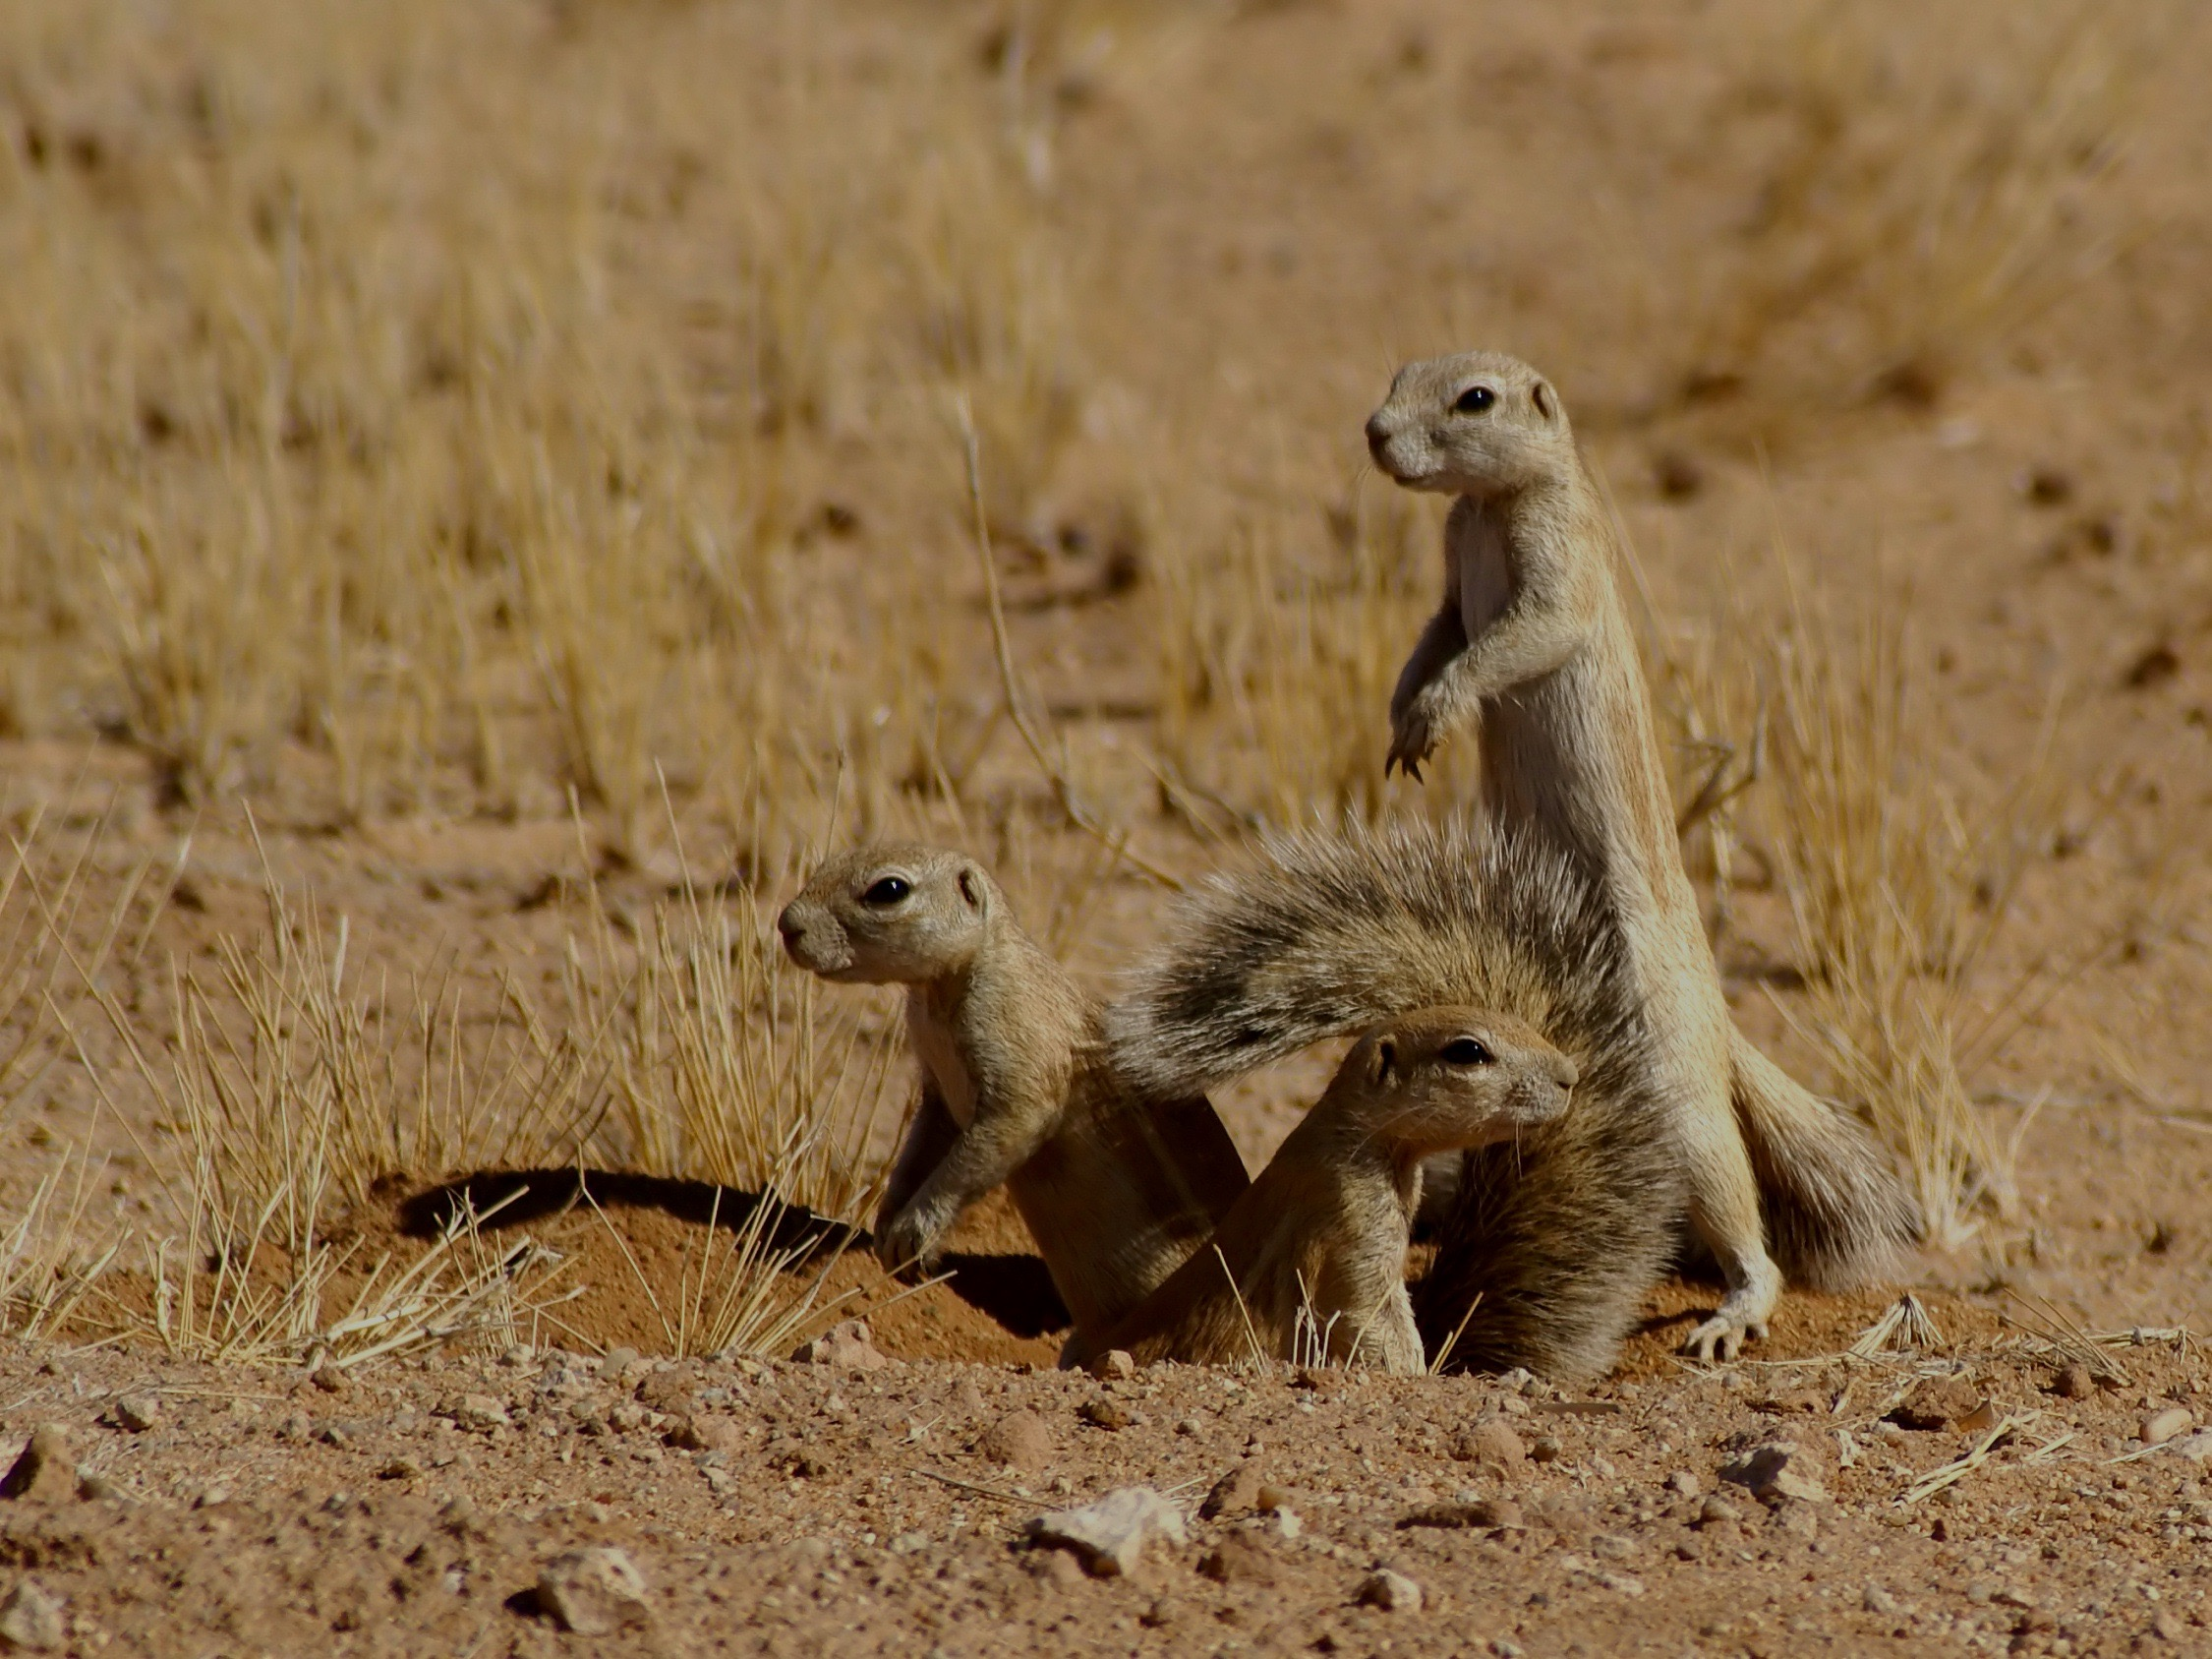
\includegraphics[width=\paperwidth,%
                   keepaspectratio=true]{images/Xerus_inauris_1}
\end{textblock*}

%% titre
\begin{textblock*}{\textwidth}(\TPHorizModule,6\TPVertModule)
  \textcolor{black!5}{\titlefmt}
\end{textblock*}

%% auteur
\begin{textblock*}{\textwidth}(\TPHorizModule,11.5\TPVertModule)
  \textcolor{black!5}{\authorfmt}
\end{textblock*}

\null\cleardoublepage

%%%
%%% Page frontispice
%%%

%% titre
\begin{textblock*}{\textwidth}(\TPHorizModule,6\TPVertModule)
  \titlefmt
\end{textblock*}

%% auteur
\begin{textblock*}{\textwidth}(\TPHorizModule,11.5\TPVertModule)
  \authorfmt
\end{textblock*}

%% affiliation
\begin{textblock*}{\textwidth}(\TPHorizModule,15.5\TPVertModule)
  \affiliation
\end{textblock*}

%% édition
\begin{textblock*}{\textwidth}(\TPHorizModule,58\TPVertModule)
  \edition
\end{textblock*}
\endgroup

%%% Local Variables:
%%% mode: latex
%%% TeX-master: "programmer-avec-r"
%%% TeX-engine: xetex
%%% End:

\null\cleartoverso              % cf. section 2.2 textpos.pdf

%%% Copyright (C) 2018 Vincent Goulet
%%%
%%% Ce fichier fait partie du projet
%%% «Programmer avec R»
%%% https://gitlab.com/vigou3/programmer-avec-r
%%%
%%% Cette création est mise à disposition selon le contrat
%%% Attribution-Partage dans les mêmes conditions 4.0
%%% International de Creative Commons.
%%% https://creativecommons.org/licenses/by-sa/4.0/

\begingroup
\calccentering{\unitlength}
\begin{adjustwidth*}{\unitlength}{-\unitlength}
  \setlength{\parindent}{0pt}
  \setlength{\parskip}{\baselineskip}
  \small

  \raisebox{-2.5mm}{%
    
\includegraphics[height=7mm,keepaspectratio=true]{images/by-sa}} %
  \raisebox{-2.5mm}{%
    
\includegraphics[height=7mm,keepaspectratio=true]{images/by-nc-sa}} %
  {\theauthor}, {\year}

  {\textcopyright} {\year} par {\theauthor}. «\thetitle», à
  l'exception les sections
  \ref*{sec:git:getting_started}--\ref*{sec:git:branching}, est mis à
  disposition selon le contrat
  \href{https://creativecommons.org/licenses/by-sa/4.0/deed.fr}{%
    Attribution-Partage dans les mêmes conditions 4.0 International}
  de Creative Commons. En vertu de ce contrat, vous êtes libre de:
  \begin{itemize}
  \item \textbf{partager} --- reproduire, distribuer et communiquer
    l'œuvre;
  \item \textbf{remixer} --- adapter l'œuvre;
  \item utiliser cette œuvre à des fins commerciales.
  \end{itemize}
  Selon les conditions suivantes:

  \begin{tabularx}{\linewidth}{@{}lX@{}}
    \raisebox{-9mm}[0mm][13mm]{%
      
\includegraphics[height=11mm,keepaspectratio=true]{images/by}}
    & \textbf{Attribution} --- Vous devez créditer l'œuvre, intégrer
    un lien vers le contrat et indiquer si des modifications ont été
    effectuées à l'œuvre. Vous devez indiquer ces informations par
    tous les moyens possibles, mais vous ne pouvez suggérer que
    l'Offrant vous soutient ou soutient la façon dont vous avez utilisé
    son œuvre. \\
    \raisebox{-9mm}{
\includegraphics[height=11mm,keepaspectratio=true]{images/sa}}
    & \textbf{Partage dans les mêmes conditions} --- Dans le cas où vous
    modifiez, transformez ou créez à partir du matériel composant
    l'œuvre originale, vous devez diffuser l'œuvre modifiée dans
    les même conditions, c'est à dire avec le même contrat avec lequel
    l'œuvre originale a été diffusée.
  \end{tabularx}

  Les sections
  \ref*{sec:git:getting_started}--\ref*{sec:git:branching} sont
  dérivées de «Pro Git» de Scott Chacon et Ben Straub sous contrat
  \href{https://creativecommons.org/licenses/by-nc-sa/3.0/deed.fr}{%
    Attribution-Pas d’utilisation commerciale-Partage dans les mêmes
    conditions 3.0 non transposé} de Creative Commons. Ce contrat
  ajoute aux conditions ci-dessus:

  \begin{tabularx}{\linewidth}{@{}lX@{}}
    \raisebox{-9mm}[0mm][13mm]{%
      
\includegraphics[height=11mm,keepaspectratio=true]{images/nc}}
    & \textbf{Pas d’utilisation commerciale} --- Vous n'êtes pas
    autorisé à faire un usage commercial de cette œuvre, tout ou
    partie du matériel la composant.
  \end{tabularx}

  \textbf{Code source} \\
  \viewsource{\reposurl}

  \textbf{Couverture} \\
  Groupe d'écureuils de terre du Cap (\emph{Xerus inauris}) sortant de
  leur terrier près de Solitaire, dans le désert du Namib, en Namibie.

  Crédit photo: {\textcopyright} Hans Hillewaert,
  \href{https://creativecommons.org/licenses/by-sa/3.0/deed.fr}{CC BY-SA 3.0}, via
  \href{https://commons.wikimedia.org/w/index.php?curid=2429056}{Wikimedia Commons}.
\end{adjustwidth*}
\endgroup

%%% Local Variables:
%%% mode: latex
%%% TeX-engine: xetex
%%% TeX-master: "programmer-avec-r"
%%% coding: utf-8
%%% End:

\clearpage

\pagestyle{companion}

%%% Copyright (C) 2020 Vincent Goulet
%%%
%%% Ce fichier fait partie du projet
%%% «Programmer avec R»
%%% https://gitlab.com/vigou3/programmer-avec-r
%%%
%%% Cette création est mise à disposition sous licence
%%% Attribution-Partage dans les mêmes conditions 4.0
%%% International de Creative Commons.
%%% https://creativecommons.org/licenses/by-sa/4.0/

\chapter{Introduction}
\markboth{Introduction}{Introduction}

Cet ouvrage traite de programmation informatique --- ou de codage,
pour utiliser le terme de plus en plus courant. À l'aube d'une
révolution numérique et de l'industrie 4.0, la programmation devient
une compétence essentielle chez les étudiants comme chez les
travailleurs du vingt-et-unième siècle. De même, la place sans cesse
grandissante accordée à la science des données --- analyse prédictive,
apprentissage profond, intelligence artificielle --- dans la plupart
des disciplines scientifiques ne fait qu'accentuer l'importance de
disposer d'une solide formation en programmation.

Les principaux buts du présent ouvrage sont donc: d'abord de
développer une culture de l'informatique; ensuite d'acquérir la
capacité à résoudre des problèmes concrets à l'aide de l'algorithmique
et de la programmation; enfin de se familiariser avec les bonnes
pratiques reconnues en contexte de travail collaboratif, puisque la
programmation se pratique beaucoup plus souvent en groupe que seul.

Vous apprendrez à programmer en R, le langage au coeur de
l'environnement statistique du même nom et l'un des outils les plus
utilisés dans le monde pour l'analyse de données. Le système R connait
depuis plus d'une décennie une progression remarquable dans ses
fonctionnalités, dans la variété de ses domaines d'application ou,
plus simplement, dans le nombre de ses utilisateurs. La documentation
sur l'utilisation de R en sciences naturelles, en sciences sociales,
en finance, etc, ne manque pas. Cependant, peu d'ouvrages se
concentrent sur l'apprentissage de R en tant que langage de
programmation sous-jacent aux fonctionnalités statistiques. C'est la
niche que je tâche d'occuper avec «Programmer avec R».

L'analyse de données requiert souvent de manipuler ou de traiter du
texte. Par conséquent, l'ouvrage aborde également les expressions
régulières et divers utilitaires d'analyse et de contrôle de texte.

Enfin, vous trouverez en annexe de brèves introductions à
l'environnement de développement intégré RStudio et à l'éditeur de
texte pour programmeurs GNU~Emacs, de même que les solutions complètes
des exercices.

\section*{Formation concomitante}

Certaines parties de l'ouvrage tablent sur des connaissances de base
dans l'utilisation d'une ligne de commande Unix et d'un système de
gestion de versions. Ma formation concomitante «Ligne de commande et
gestion de versions avec Git» \citep{Goulet:laboratoire-cli-git:2020}
permet d'acquérir ces connaissances.

La ligne de commande est la plus ancienne des interfaces avec les
ordinateurs. Si les interfaces graphiques ont à plusieurs égards
grandement facilité l'interaction homme-machine, elles n'ont pas pour
autant fait disparaitre ou rendu obsolète la ligne de commande, tout
particulièrement dans la pratique de la programmation.

Outil essentiel en contexte de travail collaboratif, le système de
gestion de versions permet de régler les problèmes de suivi de la plus
récente version d'un fichier, de partage de fichiers entre les membres
d'une équipe et de mise en commun des contributions. Développé par
Linus Torvalds pour administrer le code source du noyau du système
d'exploitation Linux, \link{https://git-scm.com}{Git} est aujourd'hui
le système de gestion de versions le plus utilisé dans le monde.


\section*{Utilisation de l'ouvrage}

L'ouvrage vise d'abord à vous exposer à un maximum de code, puis à
vous faire pratiquer. C'est pourquoi plusieurs chapitres sont rédigés
de manière synthétique et qu'ils comportent peu d'exemples au fil du
texte.

En revanche, vous devrez lire et évaluer le code informatique se
trouvant dans les sections d'exemples à la fin de la plupart des
chapitres. Ce code et les commentaires qui l'accompagnent reviennent
sur l'essentiel des concepts du chapitre et les complémentent souvent.
Je considère l'exercice d'«étude active» consistant à évaluer du code
et à voir ses effets comme essentiel à l'apprentissage de la
programmation. Vous pouvez aussi inverser la proposition et étudier le
code informatique avant le texte du chapitre correspondant si ce mode
d'apprentissage vous convient mieux.

Le code des sections d'exemples est distribué avec le document sous
forme de fichiers de script. De plus, à chaque fichier \code{.R}
correspond un fichier \code{.Rout} contenant les résultats de son
évaluation non interactive.


\section*{Fonctionnalités interactives}

En consultation électronique, ce document se trouve enrichi de
plusieurs fonctionnalités interactives.
\begin{itemize}
\item Intraliens du texte vers une ligne précise d'une section de code
  informatique et, en sens inverse, du numéro de la ligne vers le
  point de la référence dans le texte. Ces intraliens sont marqués par
  la couleur \textcolor{link}{\rule{1.5em}{1.2ex}}.
\item Intraliens entre le numéro d'un exercice et sa solution, et vice
  versa. Ces intraliens sont aussi marqués par la couleur
  \textcolor{link}{\rule{1.5em}{1.2ex}}.
\item Intraliens entre les citations dans le texte et leur entrée dans
  la bibliographie. Ces intraliens sont marqués par la couleur
  \textcolor{citation}{\rule{1.5em}{1.2ex}}.
\item Hyperliens vers des ressources externes marqués par le symbole
  {\smaller\faExternalLink*} et la couleur
  \textcolor{url}{\rule{1.5em}{1.2ex}}.
\item Table des matières, liste des tableaux, liste des figures et
  liste des vidéos permettant d'accéder rapidement à des ressources du
  document.
\item Index comprenant, entre autres, les principaux mots clés du
  langage R et toutes leurs occurrences dans le texte ainsi que
  dans le code informatique.
\end{itemize}

\section*{Blocs signalétiques}

Le document est parsemé de divers types de blocs signalétiques
inspirés de
\link{https://asciidoctor.org/docs/user-manual/\#admonition}{AsciiDoc}
qui visent à attirer votre attention sur une notion.

\tipbox{Astuce! Ces blocs contiennent un truc, une astuce, ou tout
  autre type d'information utile.}
\vspace{-\baselineskip}

\warningbox{Avertissement! Ces blocs mettent l'accent sur une notion
  ou fournissent une information importante pour la suite.}
\vspace{-\baselineskip}

\cautionbox{Attention! Vous risquez de vous bruler ---
  métaphoriquement, s'entend --- si vous ne suivez pas les
  recommandations de ces blocs.}
\vspace{-\baselineskip}

\importantbox{Important! Ces blocs contiennent les remarques les plus
  importantes. Veillez à en tenir compte.}
\vspace{-\baselineskip}

\notebox{Ces blocs contiennent des remarques additionnelles sur
  la matière ou des informations amusantes, mais non essentielles.}
\vspace{-\baselineskip}

%% Utilisation de la commande \awesomebox pour illustrer les blocs de
%% vidéos pour éviter de créer une entrée dans la liste des vidéos.
\awesomebox{\aweboxrulewidth}{\faYoutube}{url}{Ces blocs
  contiennent des liens vers des vidéos dans ma %
  \link{https://www.youtube.com/user/VincentGouletIntroR/videos}{chaine
    YouTube}. Les vidéos sont répertoriées dans la liste des vidéos.}
\vspace{-\baselineskip}

\gotorbox{Ces blocs vous invitent à interrompre la lecture du texte
  pour passer à l'étude du code R des sections d'exemples.}
\vspace{-\baselineskip}

\osxbox{Remarques spécifiques à macOS.}
\vspace{-\baselineskip}

\windowsbox{Remarques spécifiques à Windows.}

\section*{Document libre}

Tout comme R et l'ensemble des outils présentés dans ce document, le
projet «Programmer avec R» s'inscrit dans le mouvement de
l'\link{https://www.gnu.org/philosophy/free-sw.html}{informatique
  libre}. Vous pouvez accéder à l'ensemble du code source en format
{\LaTeX} en suivant le lien dans la page de copyright. Vous trouverez
dans le fichier \code{README.md} toutes les informations utiles pour
composer le document.

Votre contribution à l'amélioration du document est également la
bienvenue; consultez le fichier \code{CONTRIBUTING.md} fourni avec ce
document et voyez votre nom ajouté au fichier \code{COLLABORATEURS}.

Bonne lecture!

%%% Local Variables:
%%% mode: latex
%%% TeX-engine: xetex
%%% TeX-master: "programmer-avec-r"
%%% coding: utf-8
%%% End:


\tableofcontents
\cleartorecto
\listoftables
\cleartorecto
\listoffigures
\cleartorecto
\listofvideos

\chapter*{Comment (vraiment) bien \\ utiliser ce document}

\begin{enumerate}
\item Lire l'introduction.
\item Consulter le document dans une visionneuse PDF (Aperçu, Acrobat
  Reader) plutôt que dans un navigateur web.
\item Suivre le guide dans la lecture des chapitres. Aux avis signalés
  par le symbole {\faMapSigns}, passer à l'étude du code R des
  sections d'exemples pour revenir ensuite au texte.
\item Lire les commentaires dans les fichiers de script R et prendre
  le temps d'analyser et de bien comprendre les résultats.
\item Travailler sur les exercices seulement après avoir complété les
  étapes précédentes.
\end{enumerate}

%%% Local Variables:
%%% mode: latex
%%% TeX-engine: xetex
%%% TeX-master: "programmer-avec-r"
%%% coding: utf-8
%%% End:


%% Citation de D.E. Knuth (recto)
\cleartorecto
\thispagestyle{empty}
\begin{vplace}[0.45]
  \begin{quote}
    L'ultime test pour vérifier si je comprends quelque chose
    consiste à l'expliquer à un ordinateur. Je peux vous dire quelque
    chose et vous hocherez la tête, mais sans que je sois certain d'avoir
    bien expliqué. L'ordinateur, lui, ne hoche pas la tête. Il répète
    exactement ce que je lui ai dit. Vous pouvez faire illusion dans
    plusieurs aspects de la vie, mais pas avec les ordinateurs.
    \sourceatright{Donald E.~Knuth}
  \end{quote}
\end{vplace}

%% Vignette tirée de xkcd.com (verso)
\cleartoverso
\thispagestyle{empty}
\begin{vplace}[0.45]
  \centering
  \begin{minipage}{0.9\linewidth}
    \setkeys{Gin}{width=\textwidth}
    \includegraphics{images/compiling.png} \\
    \footnotesize\sffamily%
    Tiré de \href{https://xkcd.com/303/}{XKCD.com}
  \end{minipage}
\end{vplace}

\mainmatter

%%% Copyright (C) 2018 Vincent Goulet
%%%
%%% Ce fichier fait partie du projet
%%% «Programmer avec R»
%%% https://gitlab.com/vigou3/programmer-avec-r
%%%
%%% Cette création est mise à disposition selon le contrat
%%% Attribution-Partage dans les mêmes conditions 4.0
%%% International de Creative Commons.
%%% https://creativecommons.org/licenses/by-sa/4.0/

\chapter{Éléments d'informatique pour programmeurs}
\label{chap:informatique}

\begin{objectifs}
\item Nommer et ordonner les grands jalons de l'histoire des langages
  de programmation.
\item Identifier les principaux paradigmes de programmation.
\item Distinguer les concepts de syntaxe et de sémantique d'un langage
  de programmation.
\item Distinguer les concepts de langage compilé et de langage
  interprété.
\item Comparer les forces et faiblesses de divers langages de
  programmation en fonction de divers critères.
\item Comprendre la structure du système de fichiers d'un ordinateur
  et identifier le chemin d'accès vers une ressource dans celui-ci.
\item Naviguer dans le système de fichiers d'un ordinateur et obtenir
  une liste des fichiers à partir d'une interface en ligne de
  commande.
\end{objectifs}

Vous savez programmer.

En effet, avec l'omniprésence des outils numériques dans notre vie
quotidienne, nous automatisons tous certaines tâches:
%%
demander une alarme pour le lendemain matin;
enregistrer une émission de télé qui sera diffusée dans trois jours;
planifier des virements entre comptes chez notre institution
  financière;
signaler du contenu ou interpeller quelqu'un sur les médias sociaux
  à l'aide des symboles \code{\#} et \code{@};
entrer un code de triche dans un jeu vidéo;
calculer la moyenne d'une colonne dans un tableur;
guider un robot vers la sortie d'un labyrinthe.
%%
Vous pouvez sans doute ajouter vos propres exemples à cette liste.

Dans chacun des exemples précités, l'utilisateur dicte à une machine
des tâches à effectuer en utilisant un langage qu'elle est à même de
comprendre. Que le langage soit excessivement simple ou qu'une
interface vous guide pas à pas dans la programmation n'y change
fondamentalement rien: vous programmez.

Cet ouvrage vise simplement à vous faire atteindre un niveau de
sophistication bien plus grand qui fera réellement de vous des
programmeuses et des programmeurs informatiques.

<description du chapitre>

\section{Qu'est-ce que programmer?}
\label{sec:informatique:programmer?}

Programmer est une activité scientifique consistant d'abord et avant
tout à \emph{résoudre des problèmes}. Plutôt que d'avoir recours aux
mathématiques ou à l'expérimentation, les programmeurs demandent à une
machine de résoudre le problème pour eux. Comme le souligne
\citet{Swinnen:python:2012} --- dont la lecture du chapitre~1 est
chaudement recommandée --- programmer est «une compétence de haut
niveau, qui implique des capacités et des connaissances diverses: être
capable de (re)formuler un problème de plusieurs manières différentes,
être capable d’imaginer des solutions innovantes et efficaces, être
capable d’exprimer ces solutions de manière claire et complète.»

La première difficulté réside toutefois dans le fait de «demander» à
une machine de résoudre un problème: il faut établir un mode de
communication pour que l'humain puisse dicter des instructions à une
machine qui, en définitive, ne comprend que deux instructions: vrai et
faux, ouvert ou fermé, 0 ou 1. C'est là le rôle du \emph{langage de
  programmation}.

Tout au long de leur histoire, les humains ont inventé une multitude
de langages pour échanger entre eux: langues parlées, écritures,
langues des signes, peinture, musique, etc. Certains langages
parviennent à mieux exprimer certaines réalités ou certains sentiments
que d'autres. Or, il en va de même des langages de programmation: non
seulement sont-ils nombreux, mais certains conviennent mieux à
certains types de tâches que d'autres. Vous serez à même d'apprécier
la diversité des langages de programmation à la lecture de la
\autoref{sec:informatique:historique} qui retrace les grands jalons de
leur histoire.

\subsection{Algorithme}
\label{sec:informatique:programmer:algorithme}

Vous avez probablement déjà trié une liste de mots à l'aide d'un
ordinateur. Pourtant, l'ordinateur n'a aucune connaissance du concept
d'ordre alphabétique. Et même s'il «connaissait» cet ordre, comment au
juste réalise-t-il l'opération de tri? Ce genre de questions relève de
l'une des pierres d'assise de l'informatique:
l'\index{algorithmique}algorithmique, la science qui étudie les
algorithmes et les structures de données.

Un \index{algorithme}\emph{algorithme} est une procédure de calcul
permettant de résoudre un problème bien spécifié. En cela,
l'algorithme explique comment, à partir d'entrants, obtenir l'extrant
solution du problème. Quand on y pense, ce n'est pas très différent
d'une recette culinaire où les entrants sont les ingrédients, la
procédure les étapes de la recette et les extrants, le mets.

L'algorithmique est une discipline riche en techniques ingénieuses et
en analyses mathématiques poussées. Connaitre ses principes de base et
les algorithmes classiques permet de mieux planifier ses méthodes de
résolution de problème. En effet, un bon algorithme permet de résoudre
en quelques secondes un problème qui pourrait autrement prendre des
années.

À titre d'exemple, supposons que vous devez calculer, pour un jeu de
données quelconque, l'écart moyen des données supérieures à $12$ par
rapport à cette valeur. Un premier algorithme de très haut niveau
permettant de résoudre ce problème irait comme suit.

\begin{Schunk}
  \begin{enumerate}
  \item Sélectionner les données supérieures à $12$.
  \item Soustraire $12$ de chaque valeur retenue à la première étape.
  \item Effectuer la moyenne des valeurs obtenues à la seconde étape.
  \end{enumerate}
\end{Schunk}

Apportons une toute petite modification à l'algorithme ci-dessus.

\begin{Schunk}
  \begin{enumerate}
  \item Sélectionner les données supérieures à $12$.
  \item Effectuer la moyenne des valeurs obtenues à la première étape.
  \item Soustraire $12$ de la valeur retenue à la seconde étape.
  \end{enumerate}
\end{Schunk}

Mathématiquement, les deux approches sont tout à fait équivalentes.
Cependant, avec la première approche, nous effectuons une soustraction
pour chaque valeur supérieure à $12$ que compte jeu de données. Avec
la seconde approche, nous n'effectuons qu'une seule soustraction. Si
le jeu de données compte un million d'entrées supérieures à $12$,
c'est un million de soustractions contre une seule. En temps de
calcul, cela ne représente qu'un écart de quelques centièmes de
secondes sur un ordinateur moderne, mais ces fractions de secondes
peuvent finir par faire une différence importante lorsque la taille
des jeux de données augmente ou lorsque l'opération se répète de
nombreuses fois.

Attardons-nous à un second exemple intéressant: l'élévation d'une
valeur $b$ à la puissance $n$. Un premier algorithme, écrit cette fois
en \index{pseudo-langage}\emph{pseudo-langage}, pourrait se lire
ainsi.

\begin{Schunk}
\begin{Verbatim}
Puissance(nombre réel b, entier n)
  Si n = 0, retourner 1.
    Retourner b * Puissance(b, n - 1).
Fin Puissance
\end{Verbatim}
\end{Schunk}

Cet algorithme est \index{algorithme|récursif}\emph{récursif}: la
procédure \code{Puissance} s'appelle elle-même à répétition jusqu'à
l'obtention du résultat désiré. Mathématiquement, l'algorithme revient
à calculer $b^n$ de la manière la plus simple et intuitive qui soit:
\begin{equation*}
  b^n = b (b (b \cdots (b))).
\end{equation*}
Cela peut convenir lorsque $n$ est petit, mais peut-on faire mieux
pour une «grande» valeur de $n$? Imaginez que vous ne disposez que
d'une calculatrice munie des opérations arithmétiques de base et du
carré, et que vous devez élever un nombre à la puissance, disons,
$21$. Comment feriez-vous pour réduire le nombre d'opérations à entrer
au clavier?

\notebox{Cet exemple est moins fantaisiste qu'il n'y parait. Jusqu'au
  milieu des années 1990, les étudiants en actuariat ne disposaient
  que de ce type de calculatrice pour les examens professionnels! Le
  modèle en question de Texas Instruments était affectueusement nommé
  «TI 0».}

Vous avez pensé à un «algorithme»? Votre idée consiste fort
probablement à diviser la puissance par deux autant de fois que
possible et à élever au carré par la suite. Dans notre exemple, cela
donne
\begin{align*}
  b^{21}
  &= b (b^{20}) \\
  & = b (b^{10})^2 \\
  &= b ((b^5)^2)^2 \\
  & = b ((b (b^4))^2)^2 \\
  &= b ((b (b^2)^2)^2)^2.
\end{align*}
Ce calcul se traduit en algorithme comme suit.

\begin{Schunk}
\begin{Verbatim}
Puissance(nombre réel b, entier n)
  Si n = 0, retourner 1.
    Si n est pair, retourner (Puissance(b, n/2))^2.
    Si n est impair, retourner b * Puissance(b, n - 1).
Fin Puissance
\end{Verbatim}
\end{Schunk}

Pour élever un nombre à la puissance $21$, le premier algorithme
requiert $20$ opérations et le second, seulement $6$. Le dénombrement du
nombre d'opérations requis par un algorithme est un aspect important
de leur analyse. Il se fait généralement en notation $O()$ qui
signifie «de l'ordre de». Dans le premier algorithme de calcul de
$b^n$, le nombre d'opérations est directement proportionnel à $n$,
donc on dit que l'algorithme est $O(n)$. Dans le second algorithme où
la puissance est divisée par deux à répétition, le nombre d'opérations
est proportionnel au logarithme (en base deux) de $n$, d'où un
algorithme $O(log n)$.

\citet{Kernighan:practice:1999} font remarquer fort à propos que «si
tous les programmes reposent sur des algorithmes, très peu de
programmes exigent d'en concevoir de nouveaux». Autrement dit, aussi
complexe soit-il, un programme repose souvent sur quelques algorithmes
fondamentaux bien connus et bien établis. À ce titre, les algorithmes
de tri et de recherche jouent un rôle particulièrement important: on
estime que 25~\% du temps de calcul des ordinateurs est consacré au
tri et à la recherche! Ce n'est pour rien que Donald Knuth consacre un
volume entier de son œuvre monumentale \emph{The Art of Computer
  Programming} à ce seul sujet \citep{Knuth:ACP:vol1:1997}.


\subsection{Sémantique et syntaxe}
\label{sec:informatique:programmer:semantique}

Il y a plusieurs parallèles à dresser entre les langages de
programmation et les langues parlées ou écrites: leur apprentissage
requiert de la pratique; on en connait jamais un trop grand nombre; le
premier est plus difficile à apprendre que les suivants.
L'informatique a également emprunté à la linguistique les notions de
\index{sémantique}sémantique et de \index{syntaxe}syntaxe.

La sémantique est l'étude de ce que signifie un message ou un
programme informatique, c'est-à-dire de ce qu'il transmet ou exécute.
La syntaxe, quant à elle, étudie la structure du message ou du
programme. En simplifiant, disons que, pour une langue donnée, un
dictionnaire permet de connaitre la sémantique, alors qu'une grammaire
décrit la syntaxe \citep{Hebenstreit:semantique}.

Par exemple, exprimons le message «J'ai soif» en anglais. Dire
«\emph{I am hungry}» relèverait d'une erreur de sémantique, puisque la
signification du message s'en trouve changée. En revanche, avec
«\emph{I have thirsty}», le bon message se rendra, mais peut-être pas
sans que l'erreur de syntaxe n'ait d'abord suscité une hésitation chez
l'interlocuteur\footnote{%
  La formule correcte est «I am thirsty», soit littéralement «Je suis
  soif», en français.}.

Comme pour une langue, la maitrise d'un langage de programmation exige
de respecter à la fois les règles de sémantique et les règles de
syntaxe du langage. Le second volet est relativement facile: si le
programme compile ou s'exécute, c'est généralement que la syntaxe est
respectée. Le respect de la sémantique, ou de la manière propre d'un
langage d'exprimer des idées, demande plus d'efforts et de pratique.


\section{Bref historique des langages de programmation}
\label{sec:informatique:historique}

Ada Lovelace (1815--1852) est généralement reconnue comme la première
autrice d'un algorithme et de ce que l'on appelle aujourd'hui un
programme informatique. C'est en son honneur qu'a été nommé le langage
Ada conçu en réponse à un cahier de charges du département de la
Défense des États-Unis au début des années 1980.

Franchissons d'un bond les premiers jours de l'informatique et de la
programmation pour arriver aux ordinateurs électriques modernes, dans
les années 1940. On programme alors généralement ceux-ci en
\index{assembleur}assembleur, un langage de très bas niveau facilement
interprétable par la machine, mais difficile à lire par des humains,
comme l'extrait de programme de la
\autoref{fig:informatique:assembleur} le démontre bien.

\begin{figure}
  \centering
  \includegraphics[trim=0 475 0 0, clip=true]{images/Motorola_6800_Assembly_Language.png}
  \caption[Programme en assembleur pour un microprocesseur 8~bits
  Motorola 6800.]{Extrait d'un programme en assembleur pour un
    microprocesseur 8~bits Motorola 6800. {\small Source:
      \link{https://commons.wikimedia.org/wiki/File\%3AMotorola_6800_Assembly_Language.png}{Wikimedia
        Commons}}}
  \label{fig:informatique:assembleur}
\end{figure}

Les premiers langages créés pour transmettre des instructions à un
ordinateur apparaissent dans les années 1950. Ils sont à l'origine
intimement liés à l'architecture d'un ordinateur: à chaque type
d'ordinateur son langage de programmation. Certaines contraintes ---
ou exigences --- des langages de l'époque proviennent aussi du support
physique alors utilisé pour stocker les programmes: les cartes
perforées.

\subsection{Fortran}
\label{sec:informatique:historique:fortran}

En 1954, l'ingénieur de IBM John Backus publie les spécifications du
langage \index{Fortran}FORTRAN (\emph{FORmula TRANslating System}). Le
premier compilateur voit le jour deux ans plus tard. Fortran (avec des
minuscules à partir de 1977) deviendra rapidement le langage standard
dans le calcul scientifique.

Plus d'un demi-siècle plus tard, l'empreinte de Fortran demeure
importante, notamment grâce aux bibliothèques d'algèbre linéaire
BLAS\footnote{%
  \emph{Basic Linear Algebra Subprograms};
  \link{http://www.netlib.org/blas}{}.} %
et LAPACK\footnote{%
  \emph{Linear Algebra PACKage};
  \link{http://www.netlib.org/lapack}{}.} %
auxquelles ont recours la plupart des progiciels scientifiques, dont
R. Le langage est toujours utilisé en calcul haute performance et pour
mesurer le rendement des superordinateurs.

\notebox{Dans le très recommandable film «Les figures de l'ombre»
  (\emph{Hidden Figures}, 2016), une des héroïnes entreprend de
  s'attaquer à la programmation des nouveaux ordinateurs de la NASA.
  On peut alors voir qu'elle apprend le Fortran.}

\subsection{Lisp}
\label{sec:informatique:historique:lisp}

Le deuxième langage le plus ancien toujours largement diffusé est
\index{Lisp}Lisp (\emph{LISt Processing}). Créé par John McCarthy en
1958 en tant que modèle pratique pour représenter des programmes, le
Lisp est devenu le langage de choix pour la recherche et les
applications en intelligence artificielle. Le terme Lisp désigne
aujourd'hui une famille de langages comprenant de nombreux dialectes,
dont Common Lisp, Scheme et Emacs Lisp.

Le Lisp se distingue en outre par une syntaxe simple en
\index{notation!préfixée}notation préfixée (voir encadré), le support
pour la programmation fonctionnelle
(\autoref{sec:informatique:paradigmes}) et la faculté de manipuler le
code source en tant que structure de données. Autre trait distinctif:
la syntaxe du Lisp fait un usage immodéré des parenthèses.

Le Lisp est entouré d'une aura de beauté et d'élégance dont peu
d'autres langages peuvent se targuer. Citons Eric Raymond dans
\link{http://www.catb.org/esr/faqs/hacker-howto.html}{\emph{How to
    Become a Hacker}}:
\begin{quote}
  Il faut apprendre le Lisp pour l'extraordinaire expérience d'éveil
  [\emph{enlightenment experience}] que procure le fait de finalement
  le comprendre; cette expérience fera de vous un meilleur programmeur
  pour toujours, même si vous n'avez plus vraiment à utiliser le Lisp.
\end{quote}

Pour illustrer encore davantage la place toute particulière qu'occupe
le Lisp en programmation, mentionnons également l'aphorisme selon
lequel «ceux qui ne connaissent pas le Lisp sont condamnés à le
réinventer», d'une certaine façon la version courte de la célèbre
\link{https://en.wikipedia.org/wiki/Greenspun\%27s_tenth_rule}{\emph{Greenspun's
    tenth rule of programming}}: %
\begin{quote}
  Tout programme suffisamment complexe en C ou en Fortran comporte une
  mise en œuvre mal spécifiée, pleine de bogues et lente de la moitié
  de Common Lisp.
\end{quote}
(Fait amusant à noter: il n'y a pas d'autres lois que la dixième, de
l'\link{http://philip.greenspun.com/bboard/q-and-a-fetch-msg?msg_id=000tgU}{aveu
  même de l'auteur}.)

\begin{figure}[t]
  \label{fig:informatique:notations}
  \setlength{\FrameRule}{1pt}
  \lstset{backgroundcolor=\color{codebg},
    frame=lr, rulecolor=\color{codebg},
    xleftmargin=3.4pt, xrightmargin=3.4pt}
  \begin{emphbox}{\mdseries Notations infixée, préfixée et suffixée}
    Les notations \index{notation!infixée}infixée (\emph{infix}),
    \index{notation!préfixée}préfixée (\emph{prefix}) et
    \index{notation!suffixée}suffixée (\emph{postfix}) sont trois
    manières différentes, mais équivalentes, d'écrire des expressions
    en mathématiques ou en programmation.

    Par exemple, l'opération d'addition de deux opérandes $x$ et $y$
    s'écrit en notation infixée
\begin{lstlisting}
x + y
\end{lstlisting}
    En notation préfixée, aussi appelée notation polonaise,
    l'opérateur est placé avant les opérandes:
\begin{lstlisting}
+ x y
\end{lstlisting}
    On l'aura compris, en notation suffixée, ou notation polonaise
    inversée, l'opérateur apparait après les opérandes:
\begin{lstlisting}
x y +
\end{lstlisting}
    Nous sommes davantage habitués à lire la notation infixée, quoique
    la notation préfixée nous soit familière pour les opérateurs à un
    seul opérande (comme la négation) ou pour les appels de fonctions.
    La notation suffixée n'a jamais recours aux parenthèses.

    La compagnie HP commercialise de très prisées calculatrices
    scientifiques utilisant la notation suffixée (libellées RPN pour
    \emph{Reverse Polish Notation}) depuis 1972.
  \end{emphbox}
\end{figure}

\subsection{COBOL}
\label{sec:informatique:historique:cobol}

Le troisième langage développé dans les années 1950 et toujours en
usage de nos jours est \index{COBOL}COBOL (\emph{COmmon Business
  Oriented Language}). Ce langage spécialisé dans les applications de
gestion a été créé en 1959 par un comité formé pour proposer un
langage commun pour l'administration américaine.

Le COBOL reste très utilisé dans de grandes entreprises, notamment
dans les institutions financières. La légende urbaine veut d'ailleurs
que les programmeurs COBOL soient comparativement très bien rémunérés
aujourd'hui sous l'effet combiné de leur rareté et de l'importance
opérationnelle des applications qu'ils doivent maintenir.

\subsection{Algol}
\label{sec:informatique:historique:algol}

Dès la fin de la décennie 1950, un comité de scientifiques se réunit à
Zurich pour concevoir ce que l'on voudrait voir devenir le langage de
programmation standard. De ces rencontres naitra \index{Algol}Algol
(\emph{ALGorithmic Oriented Language}) en 1958. Comme la plupart des
tentatives de définition d'un standard, c'est un échec: le langage est
populaire dans les milieux académiques, mais restera peu utilisé dans
les applications commerciales.

Cela dit, on doit à Algol plusieurs innovations importantes, de telle
sorte qu'un grand nombre des langages qui verront le jour par la suite
seront considérés comme ses descendants; le poster
\link{http://www.oreilly.com/go/languageposter}{\emph{History of
    Programming Languages}} de O'Reilly Media illustre ceci à
merveille. \citet{Hoare:1973} a d'ailleurs cette jolie formule:
\begin{quote}
  Voici un langage très en avance sur son temps, il n'a pas seulement
  été une amélioration de ses prédécesseurs mais aussi une
  amélioration de presque tous ses successeurs.
\end{quote}

\begin{figure}[t]
  \centering
  \begin{minipage}{0.9\linewidth}
    \setkeys{Gin}{width=\textwidth}
    \includegraphics{images/standards} \\
    \footnotesize\sffamily%
    Tiré de \href{http://xkcd.com/927/}{XKCD.com}
  \end{minipage}
\end{figure}

\subsection{APL}
\label{sec:informatique:historique:apl}

Notre historique ne serait pas complet sans un mot sur \index{APL}APL
(\emph{A Programming Language}, qui l'aurait cru). Même s'il n'a
jamais connu une diffusion importante, ce langage conçu par Kenneth
Iverson autour de 1962 n'en a pas moins eu une influence considérable
sur la manière de penser et de représenter les opérations
mathématiques sur les tableaux à plusieurs dimensions.

Doté d'une large gamme de symboles pour représenter des opérations et
d'une syntaxe tout à fait particulière --- les expressions sont
exécutées de droite à gauche! --- l'APL est remarquablement concis et
puissant; voir la \autoref{fig:informatique:apl} pour un aperçu. Le
revers de la médaille et ce qui a assurément nui à son adoption
à large échelle, c'est la difficulté que l'on éprouve à relire le
code. Assez pour que d'aucuns qualifient l'APL de «langage à écriture
seulement».

APL a pendant longtemps été un langage très prisé par les actuaires,
aussi subsiste-t-il du code dans certaines compagnies d'assurance. Le
modèle de traitement des vecteurs, matrices et tableaux de l'APL a
servi d'inspiration pour la conception du langage S --- nous y
reviendrons au \autoref{chap:presentation}.

Le langage continue sa vie aujourd'hui principalement sous forme de son
successeur, \index{J}J.

\begin{figure}
  \centering
  \scalebox{0.4}{\includegraphics{images/APL_intro}}
  \caption[Opérations simples en APL.]{Opérations simples en APL. De
    haut en bas: génération des nombres de $1$ à $5$ et stockage dans
    la variable \code{x}; affichage du contenu de \code{x}; somme des
    éléments de \code{x}; moyenne des éléments de \code{x}. {\small Source:
    François-Dominique,
    \link{https://commons.wikimedia.org/w/index.php?curid=43207460}{Wikimedia
      Commons}, CC BY-SA 4.0}}
  \label{fig:informatique:apl}
\end{figure}

\subsection{C}
\label{sec:informatique:historique:c}

Le langage \index{C}C a été inventé en 1972 chez Bell Labs par Ken
Thompson et Dennis Ritchie afin de réécrire le système d'exploitation
UNIX (\autoref{sec:informatique:os:unix}). Il demeure beaucoup utilisé
pour la programmation système: le noyau de systèmes d'exploitation
comme Windows et Linux sont développés en grande partie en C.

Le C est un langage de programmation généraliste considéré, selon les
standards actuels, comme de bas niveau. Pour illustrer, l'utilisateur
doit programmer des traitements comme la libération de la mémoire, la
vérification de la validité des indices sur les tableaux, l'ouverture
et la fermeture des fichiers, etc.

Le langage demeure l'un des plus utilisés dans le monde et son
influence est considérable. De nombreux langages plus modernes comme
\index{C++@\Cpp}\Cpp, \index{C#@C\#}C\# et \index{Java}Java reprennent des
aspects de C. Le C est également beaucoup utilisé pour le calcul
numérique intensif, où il s'est en quelque sorte substitué à Fortran.
La plupart des progiciels scientifiques --- dont R, encore une fois
--- offrent la possibilité d'appeler du code C lorsque la rapidité de
calcul devient un enjeu. Le gain en temps d'exécution doit toutefois
être suffisamment grand pour compenser le temps de développement plus
long qu'exige le C par rapport à des langages de plus haut niveau.

\notebox{Dans l'ouvrage classique de \cite{KandR:1978}, le premier
  exemple d'un programme C affiche le message «\emph{hello, world}» à
  l'écran. Ça deviendra ensuite une tradition de démontrer le
  fonctionnement ou la syntaxe d'un langage avec cet exemple.}

\subsection{Autres jalons}
\label{sec:informatique:historique:autres}

Nous nous sommes attardés jusqu'ici à des langages de programmation
vieux de plus de 40 ans à cause de leur importance historique et parce
qu'ils sont toujours utilisés couramment. De nombreux autres langages
ont vu le jour depuis, si bien qu'ils se comptent aujourd'hui par
milliers. En voici quelques autres ayant occupé une place
prépondérante dans l'histoire.

\begin{itemize}
\item Comme son nom l'indique, \index{C++@\Cpp}\textbf{\Cpp} (Bjarne
  Stroustrup, 1980) est un dérivé du C qui lui ajoute, en autres
  choses, la programmation orientée objet. Certains considèrent que
  {\Cpp} devrait être le point d'entrée de toute personne voulant
  débuter à programmer avec des langages de la famille du C. Le code C
  est compatible avec le \Cpp.
\item Principal représentant de l'ère Internet des années 1990,
  \index{Java}\textbf{Java} (James Gosling, 1995) a été conçu pour
  que le code écrit dans ce langage puisse s'exécuter sur n'importe
  quelle plateforme informatique sans nécessiter une nouvelle
  compilation. Il est donc très populaire dans les applications web ou
  embarquées. Sa syntaxe est fortement inspirée du \Cpp.
\item \index{Visual Basic}\textbf{Visual Basic} (Microsoft, 1991) permet de développer des
  applications de manière interactive en disposant des composantes sur
  un canevas. Le langage est aujourd'hui discontinué, mais son dérivé
  \textbf{Visual Basic for Applications} (\index{VBA}VBA) demeure beaucoup
  utilisé dans les applications de la suite bureautique Office.
\item \index{Python}\textbf{Python} (Guido van Rossum, 1991) est un
  langage de haut niveau, orienté objet, multiplateforme et sous
  licence libre. C'est un des langages les plus utilisés aujourd'hui
  pour le calcul scientifique et l'analyse de données massives.
\end{itemize}

Certains langages de programmation ont une vocation généraliste,
certains visent des niches particulières, alors que d'autres cherchent
surtout à faire progresser l'état des connaissances dans la théorie
des langages. Quoi qu'il en soit, un langage de programmation demeure
un outil et, en informatique comme dans d'autres domaines, il convient
de choisir le meilleur outil pour accomplir une tâche donnée.

J'invite les lecteurs intéressés à en savoir davantage sur
l'histoire des langages de programmation en général, ou sur l'un ou
l'autre des langages mentionnés ci-dessus en particulier, à débuter
par les très complètes entrées de Wikipedia en
\link{https://fr.wikipedia.org/wiki/Histoire_des_langages_de_programmation}{français}
et en
\link{https://en.wikipedia.org/wiki/History_of_programming_languages}{anglais}.
\citet[chapitre~2]{Oualline:C:1997} propose également une excellente
introduction à la notion de programmation ainsi qu'une brève, mais
instructive, histoire du langage C.


\section{Langages compilés et interprétés}
\label{sec:informatique:compile_vs_interprete}

Tous les langages de programmation\footnote{%
  À l'exception du langage machine, mais rares sont les personnes qui
  souhaitent ne programmer qu'avec des $0$ et des $1$.} %
requièrent un traitement afin que les programmes écrits avec ceux-ci
puissent être exploités par un ordinateur. Il existe deux grandes
façons d'effectuer ce traitement: par compilation et par
interprétation.

Un \index{compilateur}compilateur est un programme informatique qui
transforme en langage machine le code source rédigé dans un langage
donné. On dit alors de ce langage qu'il est \index{compilé
  (langage)}\emph{compilé}. Le compilateur produit un fichier
informatique que l'ordinateur peut ensuite exécuter directement. Sur
la plateforme Windows, on reconnait notamment ces fichiers par leurs
extensions \code{.exe} ou \code{.dll}. Les noyaux d'à peu près toutes
les applications sur nos ordinateurs sont des fichiers compilés.

Un \index{interpréteur}interpréteur, quant à lui, est un programme qui
analyse, traduit et exécute le code source d'un programme
informatique, et ce, à chaque fois que le programme doit être exécuté.
Un langage qui nécessite l'intermédiaire d'un interpréteur est dit
\emph{interprété}. Un programme écrit dans un \index{interprété
  (langage)}langage interprété ne peut être distribué sans son
interpréteur.

Le traitement additionnel entre le code source et le langage machine
fait généralement en sorte que les langages interprétés sont plus
lents que les langages compilés à l'exécution. En revanche, une foule
de détails de mise en œuvre sont pris en charge par l'interpréteur, ce
qui réduit le temps de développement.


\section{Paradigmes de programmation}
\label{sec:informatique:paradigmes}

Un programme informatique est toujours écrit pour résoudre un problème
donné. Or, comme pour tout problème dans la vie, la solution à
celui-ci peut être formulée de différentes manières. Le style
fondamental avec lequel on exprime la solution est appelé le
paradigme de programmation.

Il existe plusieurs paradigmes de programmation. Nous nous
contenterons ici de se pencher sur seulement quatre.

\begin{description}
\item[Impératif] \index{paradigme!impératif} On indique à l'ordinateur
  les opérations à exécuter et l'ordre dans lequel les exécuter. C'est
  le paradigme le plus intuitif.
\item[Déclaratif] \index{paradigme!déclaratif} On indique cette fois à
  l'ordinateur ce que l'on souhaite obtenir comme résultat, mais sans
  préciser comment y parvenir. Il est laissé à la mise en œuvre du
  langage de déterminer la meilleure méthode de résolution du
  problème.

  Par exemple, pour extraire d'une base de données \code{etudiants} le
  prénom de toutes les personnes de plus de 25~ans, on écrira dans un
  langage déclaratif comme le SQL:
\begin{Schunk}
\begin{Verbatim}
SELECT prenom FROM etudiants WHERE age > 25
\end{Verbatim}
\end{Schunk}
  Nulle part n'est-il précisé comment le programme devrait procéder à
  l'extraction.
\item[Fonctionnel] \index{paradigme!fonctionnel} Un programme est une
  suite d'appels de fonctions, comme en mathématiques. L'exécution
  d'une fonction n'a pas d'impact sur les autres fonctions\footnote{%
    Autrement on dit qu'une fonction a un effet de bord (\emph{side
      effect}.} %
  Les opérations complexes sont réalisées en combinant les fonctions,
  de manière analogue à la composition de fonctions $g \circ f$.
\item[Orienté objet] \index{paradigme!orienté objet} Un programme est
  conçu comme un ensemble de blocs logiciels (les objets) qui
  interagissent entre eux. Une \emph{méthode} applique un traitement
  différent à un objet selon sa \emph{classe}. Ce paradigme est
  particulièrement utilisé dans les grands et complexes projets
  informatiques.
\end{description}

La plupart des langages d'usage courant combinent d'office, ou du
moins permettent de combiner, plusieurs paradigmes. Par exemple, le
langage {\Cpp} est à la fois un langage impératif et orienté objet.



\section{Systèmes d'exploitation}
\label{sec:informatique:os}

Le \index{système d'exploitation}système d'exploitation
(\emph{operating system}, OS) est un ensemble de programmes qui gère
les ressources matérielles et logicielles d'un ordinateur. Premier
programme exécuté par l'ordinateur lors de la mise en marche, le
système d'exploitation reçoit les demandes de ressources des
applications --- espace mémoire, unité de calcul, disque dur,
communication avec les périphériques, utilisation du réseau --- et les
alloue en fonction de l'état du système et des demandes concurrentes
des autres applications. Tous les logiciels applicatifs requièrent un
système d'exploitation pour fonctionner.

Il existe une grande variété de systèmes d'exploitation. Les plus
connus aujourd'hui sont, pour les ordinateurs personnels et les
serveurs, Windows de Microsoft, macOS de Apple et Linux, un logiciel
libre créé et toujours administré par Linus Torvalds. Pour les
appareils mobiles, deux systèmes d'exploitation se partagent
l'essentiel du marché: iOS et Android. Le premier est dérivé de macOS
et le second, de Linux.

Les systèmes macOS et Linux appartiennent à la famille des systèmes
Unix. Cela ne laisse donc en fait que deux grandes classes de systèmes
d'exploitation couramment utilisés: Windows et Unix.

\subsection{Windows}
\label{sec:informatique:os:windows}

Le système d'exploitation \index{Windows}Windows de Microsoft équipe
près de 90~\% des ordinateurs personnels dans le monde. Dans les
circonstances, rares sont les personnes qui n'ont jamais utilisé le
système, ne serait-ce qu'à petites doses.

À l'origine, en 1985, Windows n'était qu'une interface graphique
superposée au véritable système d'exploitation des ordinateurs de type
«compatibles IBM PC», le DOS. Les versions grand public depuis
Windows~2000 sont plutôt basées sur le noyau de Windows~NT, un système
conçu à partir de zéro et lancé au milieu des années 1990 en tant que
système pour les entreprises.

Le plus grand avantage de Windows est son ubiquité. À peu près toutes
les applications, sauf peut-être celles s'adressant à un segment de
marché très précis, sont disponibles sous Windows, en code natif, via
un port depuis Unix, ou encore par l'intermédiaire d'une couche
logicielle d'émulation comme Cygwin ou \index{MinGW}MinGW.

Un système d'exploitation multiutilisateur prend pour acquis que
plusieurs utilisateurs se partageront les ressources de l'ordinateur,
simultanément lorsqu'il s'agit d'un serveur, ou les uns après les
autres dans le cas d'un ordinateur personnel. Dans un tel système, on
établit des règles strictes d'accès aux ressources du système (seul
l'administrateur peut installer ou supprimer des applications) et
d'accès aux ressources des autres utilisateurs (Marianne n'a pas
accès aux fichiers d'Alexandre et vice-versa).

Les versions de Windows multiutilisateurs sont apparues relativement
tard sur le marché grand public, et ce, sans que le paradigme ne soit
imposé aux utilisateurs. Résultat: la plupart des utilisateurs de
Windows s'octroient à la ronde les droits d'administrateur et, pire,
plusieurs applications nécessitent toujours un accès total au système.
C'est par ces failles que se propagent virus et autres logiciels
malveillants sur la plateforme.

Les systèmes Windows sont livrés avec une trousse de développement
très restreinte. Les programmeurs doivent donc installer les outils
nécessaires, souvent sous forme de suites logicielles monolithiques,
ce qui entraine dédoublements et, parfois, conflits.

\subsection{Unix}
\label{sec:informatique:os:unix}

Le terme \index{Unix}\emph{Unix} --- ou UNIX qui, en majuscules, est
une marque déposée de \link{http://www.opengroup.org/unix}{Open Group}
--- recoupe une famille de systèmes d'exploitation dérivant tous du
premier système Unix développé chez Bell Labs dans les années 1970 par
Kenneth Thompson, Dennis Ritchie et plusieurs autres.

Les systèmes Unix partagent un certain nombre de caractéristiques
communes. D'abord, ils sont intrinsèquement multitâches et
multiutilisateurs. Ensuite, la
\Index{Unix!philosophie}\link{https://fr.wikipedia.org/wiki/Philosophie_d\%27Unix}{philosophie
  Unix} commande la modularité: le système d'exploitation fournit aux
utilisateurs (via un interpréteur de commandes, ou \emph{shell}) et
aux applications une multitude de petits outils très spécialisés qui
ne réalisent à peu près qu'une seule tâche. Le système rend ensuite
simple, via un mécanisme dit de transfert de données («tuyau»,
\emph{pipe}) de les combiner pour effectuer des opérations plus
complexes.

Par exemple, pour extraire le mot \emph{tuyau} du code source
contenant le précédent paragraphe, nous pourrions utiliser l'outil
\code{grep} pour extraire la ligne où se trouve le mot, puis l'outil
\code{cut} pour isoler le mot qui nous intéresse et, enfin, l'outil
\code{tr} pour supprimer la parenthèse ouvrante, les guillemets et la
virgule autour du mot.\footnote{%
  Dans la mesure où le mot que l'on recherche est le quatrième de la
  ligne dans le fichier source \code{informatique.tex}, la commande
  résultante est: \code{grep "«tuyau»" informatique.tex | cut -d " "
    -f 4 | tr -d \bs(«»,}\,. Le caractère \code{|} est l'opérateur de
  transfert de données.}

À l'exception notable des Mac, \index{Unix}Unix demeure assez peu répandu sur les
ordinateurs personnels. En revanche le système d'exploitation, en
particulier sa variante libre Linux, équipe l'immense majorité des
stations de travail, serveurs et supercalculateurs. De plus, bon
nombre d'applications scientifiques et de langages de programmation
sont d'abord développés sur des systèmes Unix. Pour ces
raisons, j'estime utile pour des programmeurs de connaitre les
quelques «Unix-ismes» ci-dessous.

\begin{itemize}
\item La barre oblique (\code{/}) est utilisée pour séparer les
  dossiers dans les chemins d'accès aux fichiers.
\item Tout utilisateur dispose d'un espace disque réservé identifié
  comme le \index{répertoire personnel}\emph{répertoire personnel} ou
  le \index{dossier de départ|see{répertoire personnel}}\emph{dossier
    de départ} (\emph{home directory}). Ce répertoire est situé dans
  \code{/Users} sous macOS et habituellement dans \code{/home} sous
  Linux.
\item À la ligne de commande et dans la configuration de plusieurs
  applications, le caractère \,\verb=~=\, représente le répertoire
  personnel.
\item Toujours à la ligne de commande, il est possible d'appuyer sur
  \code{TAB} pour compléter les noms de fichiers, de répertoires ou de
  commandes.
\item Plusieurs applications permettent de stocker des options de
  configuration sous forme de texte brut dans des fichiers dont le nom
  débute généralement par un point «\verb=.=»\,.
\end{itemize}
La section suivante fournit des détails additionnels sur le système de
fichiers de Unix.


\section{Systèmes de fichiers}
\label{sec:informatique:fs}

Le \index{système de fichiers}système de fichiers d'un ordinateur
contrôle l'inscription, l'organisation et la récupération des données
sur une unité de stockage, souvent un disque dur.

Nous n'entrerons pas dans les détails techniques des systèmes de
fichiers. Seulement, les programmeurs doivent être familiers avec
quelques grands principes de l'organisation des données dans un
ordinateur.

Les fichiers sont regroupés dans des répertoires. Ceux-ci contiennent
eux-mêmes des fichiers ou des sous-répertoires. Ce schéma se répète
sans limite pratique. Il en résulte une classification sous forme
d'arbre dont la \emph{racine} est le répertoire contenant
l'intégralité des fichiers. La \autoref{fig:informatique:fs} présente
des extraits des arbres de fichiers usuels de Windows et de macOS.

\begin{figure}
  \begin{minipage}[t]{0.45\linewidth}
    \dirtree{%
      .1 \code{C:\bs}.
      .2 \code{Program Files\bs}.
      .3 \code{Internet Explorer\bs}.
      .3 \code{Windows NT\bs}.
      .2 \code{Users\bs}.
      .3 \code{Alexandre\bs}.
      .4 \code{Desktop\bs}.
      .4 \code{Documents\bs}.
      .5 \code{synthese-1.doc}.
      .2 \code{Windows\bs}.
      .3 \code{explorer.exe}.
      .3 \code{System32\bs}.
      .4 \code{wininit.exe}.
    }
  \end{minipage}
  \hfill
  \begin{minipage}[t]{0.45\linewidth}
    \dirtree{%
      .1 \code{/}.
      .2 \code{/Applications}.
      .3 \code{/Mail.app}.
      .3 \code{/Preview.app}.
      .2 \code{/Users}.
      .3 \code{/Marianne}.
      .4 \code{/Desktop}.
      .5 \code{freestyle.txt}.
      .4 \code{/Documents}.
      .5 \code{/Cours}.
      .2 \code{/System}.
      .2 \code{/bin}.
      .3 \code{bash}.
      .2 \code{/usr}.
      .3 \code{/bin}.
      .4 \code{grep}.
    }
  \end{minipage}
  \caption[Extraits de la hiérarchie des systèmes de fichiers]{%
    Extraits des arbres de fichiers de Windows~7 (à gauche) et de
    macOS (à droite)}
  \label{fig:informatique:fs}
\end{figure}

\subsection{Particularités du système de fichiers de Windows}
\label{sec:informatique:fs:windows}

Sous Windows, chaque lecteur physique ou lecteur réseau dispose de son
propre arbre de fichiers. La racine est identifiée par une lettre. Le
premier disque dur est \code{C}\footnote{%
  La nomenclature des lecteurs date d'une époque où les ordinateurs
  personnels n'étaient pas tous équipés d'un disque dur, mais plutôt
  d'un ou deux lecteurs de disquettes. Ceux-ci étaient identifiés par
  les lettres \code{A} et \code{B}.}. %
Si le système comporte plus d'un disque, l'utilisateur doit savoir sur
quel disque retrouver ou enregistrer ses données.

Le système de fichiers de Windows est insensible à la casse,
c'est-à-dire qu'il ne fait aucune distinction entre \code{Program
  Files}, \code{program files} et \code{PROGRAM FILES}. Dans les
chemins d'accès (voir ci-dessous), la barre oblique inversée
{\bs} sépare les noms de répertoires.

\subsection{Particularités du système de fichiers de Unix}
\label{sec:informatique:fs:unix}

La racine du système de fichiers est toujours \code{/} sous
\index{Unix}Unix. Les disques, physiques ou réseau, sont accessibles
par divers \emph{points de montage} dans le système de fichiers.

Pour illustrer, supposons qu'un ordinateur dispose de deux disques
durs; le premier est réservé au système d'exploitation et aux
applications partagées, alors que le second renferme les fichiers
personnels des utilisateurs. Dans un tel scénario, le premier disque
sera monté sur le répertoire \code{/} et le second, sur le répertoire
\code{/home}. Le système de fichier dirigera automatiquement les
requêtes vers le bon disque. L'utilisateur n'a jamais à se préoccuper
de l'organisation physique des disques.

\osxbox{Sous macOS, les clés USB, disques durs externes ou disques réseau sont
  montés dans le répertoire \code{/Volumes}. Le répertoire
  n'existe pas lorsqu'aucun disque externe n'est connecté.}

Le système de fichiers sous Unix est généralement sensible à la casse.
La barre oblique \code{/} sépare les noms de répertoires dans les
chemins d'accès.

Les fichiers dont le nom débute par un point «\verb=.=» sont des
fichiers cachés. À moins de demander explicitement de les afficher,
ils n'apparaissent donc pas dans la liste des fichiers à la ligne de
commande ou dans les interfaces graphiques.

\subsection{Chemin d'accès}
\label{sec:informatique:fs:path}

Le \index{chemin d'accès}chemin d'accès (\emph{path}) d'un fichier ou
d'un répertoire décrit la position de la ressource dans le système de
fichiers. Un chemin d'accès peut être absolu ou relatif.
\begin{description}
\item[Chemin absolu] \index{chemin d'accès!absolu} La position d'un
  fichier est décrite à partir de la racine, de telle sorte que le
  chemin d'accès demeure valide depuis n'importe quel point dans le
  système de fichier.

  Dans l'extrait de système de fichier Windows de la
  \autoref{fig:informatique:fs}, le chemin d'accès absolu vers le
  fichier \code{synthese-1.doc} est:
\begin{Schunk}
\begin{Verbatim}
C:\Users\Alexandre\Documents\synthese-1.doc
\end{Verbatim}
\end{Schunk}
\item[Chemin relatif] \index{chemin d'accès!relatif} La position d'un
  fichier est donnée à partir d'un endroit précis dans le système de
  fichier autre que la racine. Le chemin dépend donc du répertoire
  courant. On a recours au nom fictif «\verb=..=» pour identifier le
  répertoire parent (un niveau supérieur dans l'arbre des fichiers).

  Par exemple, si le répertoire courant de Marianne est
  \code{Documents/Cours} dans le système de fichier Unix de la
  \autoref{fig:informatique:fs}, alors le chemin d'accès relatif vers
  le fichier \code{freestyle.txt} est:
\begin{Schunk}
\begin{Verbatim}
../../Desktop/freestyle.txt
\end{Verbatim}
\end{Schunk}
\end{description}

La notion de chemin d'accès fait également référence à la liste des
répertoires dans lesquels le système d'exploitation recherche une
application lorsqu'elle est appelée. Cette liste est conservée dans
une variable d'environnement nommée \verb=%PATH%= sous Windows
et \verb=$PATH= sous \index{Unix}Unix. Il est hors de la portée de ce
document d'expliquer comment modifier la variable d'environnement. La
réponse se trouve à une requête près dans un moteur de recherche.


\section{Ligne de commande}
\label{sec:informatique:cli}

Une interface en \index{ligne de commande}ligne de commande
(\emph{command line interface}, CLI), ou tout simplement \emph{ligne
  de commande}, est un mode d'interaction avec un programme
informatique dans lequel l'utilisateur dicte les commandes et reçoit
les réponses de l'ordinateur en mode texte. Le programme qui gère
cette interface est un \emph{interpréteur de commandes}, parfois aussi
appelé (à tort) \emph{terminal} ou \emph{shell}. Lorsque
l'interpréteur est prêt à recevoir une commande, il l'indique par une
\emph{invite de commande} (\emph{command prompt}).

La ligne de commande est la plus ancienne des interfaces avec les
ordinateurs. Si les interfaces graphiques ont à plusieurs égards
grandement facilité l'interaction homme--machine, elles n'ont pas pour
autant fait disparaitre ou rendu obsolète la ligne de commande.
D'abord, celle-ci demeure parfois la seule --- et souvent la plus
rapide --- interface pour réaliser certaines tâches sur un ordinateur
muni d'une interface graphique. Ensuite, certains ordinateurs, comme
les serveurs ou les supercalculateurs, n'offrent souvent aucune
interface graphique.

\subsection{Ligne de commande Windows}
\label{sec:informatique:cli:windows}

L'interpréteur de commandes standard sous Windows est
\index{cmd@\code{cmd.exe}}\code{cmd.exe}. On le trouve dans le groupe
de programmes \code{Accessoires} sous le nom \code{Invite de
  commandes}. L'invite de commande par défaut est \verb=C:\>=. À la
gauche du symbole \verb=>= se trouve le chemin d'accès du répertoire
courant. Au lancement de l'interpréteur, celui-ci est donc la racine
du système de fichiers.

Les programmeurs qui souhaitent bénéficier de certains outils
\index{Unix}Unix sous Windows peuvent installer les couches
logicielles \index{MinGW}MinGW et \index{MSYS}MSYS --- je recommande à
cet égard la distribution
\link{http://www.msys2.org}{MSYS2}\index{MSYS2}. Le programme
\code{MSYS} fournit un interpréteur de commandes \index{Bash}Bash
\citep{bash} comme en standard sur les systèmes Unix. Un interpréteur
Bash est également fourni avec \index{Git}
\link{https://git-scm.com/downloads}{Git for Windows}: le programme
est d'ailleurs nommé \index{Git~Bash}Git~Bash.

À la ligne de commande \index{Unix}Unix sous Windows, on identifie la
racine \code{C:\bs} du système de fichier d'un disque par \code{/c/}.

\subsection{Ligne de commande macOS}
\label{sec:informatique:cli:macos}

Sous macOS, l'application de ligne de commande se nomme
\index{Terminal}Terminal. Elle se trouve dans le sous-dossier
Utilitaires du dossier Applications. L'interpréteur de commandes est
\index{Bash}Bash. L'invite de commande par défaut est le symbole
\verb=$=, habituellement précédé du nom de l'ordinateur, du répertoire
courant et du nom de l'utilisateur. Le répertoire courant au lancement
de l'interpréteur est le répertoire personnel \,\verb=~=\, de
l'utilisateur.

\tipbox{Explorez les préférences de l'application
  \index{Terminal}Terminal pour configurer la police de caractères et
  les couleurs afin de rendre la ligne de commande plus agréable à
  utiliser.}

\subsection{Commandes essentielles}
\label{sec:informatique:cli:commandes}

Les programmeurs doivent connaitre les rudiments de la ligne de
commande. Cela dit, comme nous ne pouvons nous étendre sur le sujet,
limiterons la présentation aux commandes ci-dessous qui
permettent de se déplacer dans le système de fichiers et d'afficher
la liste des fichiers d'un répertoire.

\importantbox{Dans les exemples ci-dessous et pour le reste du
  document, l'invite de commande du système d'exploitation sera
  représentée par le symbole \code{\$} précédé du nom du répertoire
  courant (lorsque cela s'avère pertinent).}

\begin{ttscript}{pwd}
\item[\Icode{cd}] Change le répertoire courant pour
  celui donné en argument. Cet argument peut être un chemin d'accès
  absolu ou relatif (\autoref{sec:informatique:fs:path}). Le nom
  fictif «\verb=..=» identifie le parent du répertoire courant.

  Lorsque utilisée sans argument, la commande affiche le chemin
  d'accès absolu du répertoire courant avec \code{cmd.exe}, ou ramène
  directement l'invite de commande au répertoire personnel de
  l'utilisateur avec Bash.
  \begin{Schunk}
\begin{Verbatim}
~$ cd Desktop/
/Users/vincent/Desktop
~/Desktop$ cd ~/Documents/cours/
~/Documents/cours$ cd
~$
\end{Verbatim}
  \end{Schunk}
\item[\Icode{pwd}] (\index{Bash}Bash seulement) Affiche le chemin
  d'accès absolu du répertoire courant.
  \begin{Schunk}
\begin{Verbatim}
~$ pwd
/Users/vincent
\end{Verbatim}
  \end{Schunk} %$
\item[\Icode{dir}] (\index{cmd@\code{cmd.exe}}\code{cmd.exe}
  seulement) Affiche les fichiers du répertoire donné en argument, ou
  les fichiers du répertoire courant sans aucun argument.
\item[\code{ls}] \Index{ls@\code{ls} (Bash)} (\index{Bash}Bash
  seulement) Affiche les fichiers du répertoire donné en argument, ou
  les fichiers du répertoire courant sans aucun argument.
  \begin{Schunk}
\begin{Verbatim}[commandchars=\\\{\}]
~$ ls
Desktop
Documents
Downloads
\meta{...}
\end{Verbatim}
  \end{Schunk} %$
\end{ttscript}

\tipbox{Les systèmes d'exploitation affichent certains répertoires
  (\code{Bureau} ou \code{Musique}, par exemple) dans la langue de
  l'interface plutôt que sous leur vrai nom anglais. La commande
  \code{ls} affiche toujours le véritable nom des répertoires.}

\section{Exercices}
\label{operateurs:exercices}

\Opensolutionfile{solutions}[solutions-informatique]

\begin{Filesave}{solutions}
\section*{Chapitre \ref*{chap:informatique}}
\addcontentsline{toc}{section}{Chapitre \protect\ref*{chap:informatique}}

\end{Filesave}

\begin{exercice}[nosol]
  Des nouveaux langages de programmation apparaissent régulièrement.
  Deux exemples récents provenant de géants de l'industrie sont
  \link{https://swift.org}{Swift}, de Apple, et
  \link{https://golang.org}{Go}, de Google. À partir des informations
  glanées sur les sites Internet des langages et dans les pages
  Wikipedia qui leurs sont consacrées, retracer les grands langages
  ayant servi comme sources d'inspiration à \index{Swift}Swift et à
  \index{Go}Go.
\end{exercice}

\begin{exercice}
  Soit $A$, $B$, $C$ et $D$ quatre nombres. L'opération en notation
  infixée
  \begin{equation*}
    A \times B + C \div D
  \end{equation*}
  s'écrit
  \begin{equation*}
    +\, \times\, A\; B\, \div\, C\; D
  \end{equation*}
  en notation préfixée et
  \begin{equation*}
    A\; B\, \times\, C\; D\, \div +
  \end{equation*}
  en notation suffixée.
  \begin{enumerate}
  \item Exprimer en notations préfixée et suffixée l'opération en
    notation infixée suivante:
    \begin{equation*}
      A \times (B + C) \div D.
    \end{equation*}
  \item Les opérations suivantes exprimées en notation préfixée et
    suffixée, dans l'ordre, effectuent la même opération arithmétique.
    \begin{gather*}
      \times\, A\, +\, B\, \div\, C\; D \\
      A\; B\; C\; D\, \div +\, \times
    \end{gather*}
    Exprimer cette opération en notation infixée.
  \end{enumerate}
  \begin{sol}
    \begin{enumerate}
    \item $\div \times\, A\, +\, B\; C\; D$ en notation préfixée;
      $A\; B\; C\, +\, \times\, D\, \div$ en notation suffixée.
    \item $A \times (B + C \div D)$
    \end{enumerate}
  \end{sol}
\end{exercice}

\begin{exercice}
  Démarrer un interpréteur de commandes Bash. Si le système
  d'exploitation de votre ordinateur est Windows, vous pouvez utiliser
  la ligne de commande \index{Git~Bash}Git~Bash de
  \link{https://git-scm.com/downloads}{\emph{Git for Windows}} ou la
  ligne de commande MSYS de
  \index{MSYS2}\link{http://www.msys2.org}{MSYS2}.
  \begin{enumerate}
  \item Afficher le répertoire courant. Vérifier qu'il correspond à
    celui mentionné dans l'invite de commande. Localiser ce répertoire
    dans l'interface graphique de votre système d'exploitation (Finder
    sous macOS, Windows~Explorer sous Windows).
  \item Afficher la liste des fichiers du répertoire courant.
  \item Choisir un sous-répertoire du répertoire courant que vous
    savez contenir lui-même un sous-répertoire (par exemple:
    \code{Documents/Cours}. Afficher, sans d'abord s'y déplacer, la
    liste des fichiers du premier sous-répertoire (\code{Documents}),
    puis celle du second (\code{Cours}).
  \item Faire du sous-répertoire utilisé précédemment le répertoire
    courant.
  \item Afficher une liste détaillée des fichiers du nouveau
    répertoire courant avec la commande \verb=ls -l=.
  \item Descendre d'un autre niveau dans l'arbre des fichiers.
  \item Revenir au répertoire personnel avec une seule commande.
  \item Afficher la liste de tous les fichiers du répertoire
    personnel, y compris les fichiers cachés, avec la commande
    \verb=ls -a=.
  \item Afficher la liste détaillée de tous fichiers du répertoire
    personnel avec la commande \verb=ls -la=.
  \item Afficher la liste des répertoires dans lesquels le système
    d'exploitation recherche des applications avec la commande
    \verb=echo $PATH=.
  \end{enumerate}
  \begin{sol}
    Vous trouverez ci-dessous une transcription (partielle) de la
    séance de travail à effectuer depuis une ligne de commande Bash.
    \begin{Schunk}
\begin{Verbatim}[commandchars=\\\{\}]
\textbf{~$} pwd
/Users/vincent
\textbf{~$} ls
Desktop           Music        emacs-modified-extensions
Documents         Pictures     emacs-modified-macos
Downloads         Public       emacs-modified-windows
\meta{...}
\textbf{~$} ls Documents/
Spoon-Knife
actexam
actuar
actuarialangle
actuarialsymbol
\meta{...}
\textbf{~$} ls Documents/cours/
ACT-2002        ACT-2005        ACT-2008        IFT-1902
\textbf{~$} cd Documents/
/Users/vincent/Documents
\textbf{~/Documents$} ls -l
drwxr-xr-x   6 vincent staff 204 29 nov 14:40 Spoon-Knife
drwxr-xr-x   6 vincent staff 204 21 nov  2016 actexam
drwxr-xr-x  10 vincent staff 340  1 sep 09:56 actuar
\meta{...}
\textbf{~/Documents$} cd cours/
/Users/vincent/Documents/cours
\textbf{~/Documents/cours$} cd
\textbf{~$} ls -a
.                     .bashrc           .profile
..                    .cache            .rstudio-desktop
.CFUserTextEncoding   .cups             .subversion
\meta{...}
\textbf{~$} ls -la
total 584
drwxr-xr-x@ 71 vincent staff  2414  4 déc 21:03 .
drwxr-xr-x   5 root    admin   170 19 oct 04:13 ..
drwxr-xr-x   4 vincent staff   136 10 mai  2017 .R
-rw-r--r--   1 vincent staff    63  5 jul  2013 .Renviron
-rw-r--r--   1 vincent staff 23185  9 nov 09:13 .Rhistory
-rw-r--r--   1 vincent staff    71  4 jan  2016 .Rprofile
\meta{...}
\textbf{~$} echo PATH
/opt/local/bin:/opt/local/sbin:~/bin:/usr/local/bin:
/usr/bin:/bin:/usr/sbin:/sbin:/Library/TeX/texbin
\end{Verbatim}
    \end{Schunk}
  \end{sol}
\end{exercice}

\Closesolutionfile{solutions}

%%% Local Variables:
%%% mode: latex
%%% TeX-engine: xetex
%%% TeX-master: "programmer-avec-r"
%%% coding: utf-8
%%% End:

%%% Copyright (C) 2019 Vincent Goulet
%%%
%%% Ce fichier fait partie du projet
%%% «Programmer avec R»
%%% https://gitlab.com/vigou3/programmer-avec-r
%%%
%%% Cette création est mise à disposition sous licence
%%% Attribution-Partage dans les mêmes conditions 4.0
%%% International de Creative Commons.
%%% https://creativecommons.org/licenses/by-sa/4.0/

\chapter{Algorithmes et algorithmique}
\label{chap:algorithmes}

\def\scriptfilename{\currfilebase.R}

\begin{objectifs}
\item Résoudre un problème sous la forme d'un algorithme en langage
  naturel ou en pseudocode.
\item Utiliser des instructions conditionnelles dans un algorithme.
\item Utiliser la récursion et l'itération pour effectuer des tâches
  répétitives dans un algorithme.
\item Évaluer la performance d'un algorithme à l'aide de la notation
  $O()$.
\end{objectifs}

Marianne et Alexandre doivent fournir une solution logicielle à un
problème donné. Sitôt la lecture de l'énoncé du problème complétée,
ils se précipitent sur le clavier pour coder leur solution. Rapidement
bloqués, pensant qu'ils butent sur un problème de syntaxe ou
d'utilisation d'une fonction, ils demandent de l'aide. Lorsqu'on leur
demande qu'est-ce qu'ils essaient de faire, quelle est la nature de leur
solution, ils ne peuvent répondre que par un long silence.

Dans mon rôle de professeur, j'ai été témoin de la scène ci-dessus à
de nombreuses reprises. Marianne et Alexandre font une erreur commune
chez les programmeurs --- et pas que chez les débutants: commencer à
coder sans avoir au préalable suffisamment réfléchi à la solution. Il
leur manque un plan clair des étapes à suivre pour résoudre le
problème. Or, ce plan, ou la recette à suivre pour transformer les
entrants d'un problème en une solution, c'est
l'\index{algorithme}\emph{algorithme}. Travailler sans algorithme,
c'est comme naviguer sans boussole.

Puisque programmer requiert des algorithmes, l'étude de la
programmation doit par conséquent s'accompagner de notions
d'\index{algorithmique}\emph{algorithmique}, la science qui étudie les
algorithmes et les structures de données. L'algorithmique est une
discipline riche en techniques ingénieuses et en analyses
mathématiques poussées. Connaitre ses principes de base et étudier
certains algorithmes classiques vous permettra de mieux planifier vos
méthodes de résolution de problème. En effet, un bon algorithme permet
de résoudre en quelques secondes un problème qui pourrait autrement
prendre des années.

L'étude des algorithmes s'accompagne habituellement de celle des
structures de données ou, en d'autres termes, de la manière
d'organiser les données dans un ordinateur. Comme nous le verrons au
\autoref{chap:donnees}, il existe bien différentes structures de
données en R, mais leur réelle mise en œuvre demeure tout à fait
transparente pour les programmeuses et les programmeurs. C'est
pourquoi nous ferons l'impasse sur des notions que l'on retrouve dans
tous les ouvrages classiques d'algorithmique, comme le tableau
(\emph{array}), la liste chainée (\emph{list}), l'arbre (\emph{tree})
ou la table de hachage (\emph{hashtable}).

Le présent chapitre est inspiré de \citet{Sussman:scheme:1996},
\citet{Knuth:ACP:vol1:1997} et \citet{Stephens:algorithms:2013}.


\section{Définition et analogie}
\label{sec:algorithmes:definition}

Un \index{algorithme}algorithme est une procédure de calcul
permettant de résoudre un problème bien spécifié. L'algorithme
explique, de manière non ambigüe et dans un nombre d'opérations fini,
comment, à partir d'entrants, obtenir l'extrant solution du problème.

Pour se mériter un algorithme, un problème doit renfermer une dose
minimale de complexité: personne n'écrit un algorithme pour extraire
le quatrième élément d'un vecteur de données. On suppose que cela fait
partie de la définition de vecteur et que vous savez comment effectuer
l'opération dès lors que vous connaissez le langage de programmation
sous-jacent.

Dans la même veine, un algorithme ne dépend pas du langage de
programmation employé car il fournit les étapes pour résoudre un
problème, non pas leur mise en œuvre. En d'autres termes, un
algorithme explique \emph{ce qu'il faut faire} pour résoudre un
problème et non \emph{comment le faire}.

Illustrons le concept d'algorithme par l'un de ses plus illustres
représentants: l'\Index{Euclide@Euclide (algorithme)}algorithme
d'Euclide (c.~300 av. J.-C.), une procédure de calcul du plus grand
commun diviseur (PGCD) de deux nombres entiers $m$ et $n$.
L'algorithme repose sur l'idée que le PGCD de $m$ et $n$ est aussi le
PGCD de $n$ et du reste de la division de $m$ par $n$.

\begin{algorithme}[Algorithme d'Euclide]
  \label{algo:algorithmes:euclide}
  Calculer le plus grand commun diviseur de deux entiers positifs $m$
  et $n$ avec, sans perte de généralité, $n < m$.
  \begin{enumerate}
  \item Diviser $m$ par $n$ et poser $r$ égal au reste de la division.
    (Nous avons alors $0 \leq r < n$.)
  \item Si $r = 0$, retourner la valeur $n$.
  \item Poser $m \leftarrow n$, $n \leftarrow r$, puis retourner à
    l'étape 1.
  \end{enumerate}
\end{algorithme}

Suivons les étapes de l'\index{Euclide@Euclide (algorithme)}algorithme
d'Euclide avec $m = 544$ et $n = 119$. À l'étape~1, nous déterminons
que $544/119 = 4 + 68/119$, donc nous posons $r \leftarrow 68$.
Puisque $r \neq 0$, l'étape~2 de l'algorithme ne s'applique pas. Nous
passons donc à l'étape~3 et nous posons $m \leftarrow 119$ et
$n \leftarrow 68$. De retour à l'étape~1, nous déterminons cette fois
que $r \leftarrow 51$, ce qui mène encore à l'étape~3 et
$m \leftarrow 68$ et $n \leftarrow 51$. Après un autre cycle, nous en
sommes à $m \leftarrow 51$ et $n \leftarrow 17$. Cette fois, nous
posons $r \leftarrow 0$ à l'étape~1 et la procédure s'arrête ensuite à
l'étape~2. Le plus grand commun diviseur de $544$ et $119$ est $17$.
Le \autoref{tab:algorithmes:euclide} dresse le sommaire des opérations
ci-dessus.

\begin{table}
  \centering
  \caption{Calcul du plus grand commun diviseur de $544$ et $119$ avec
    l'algorithme d'Euclide}
  \label{tab:algorithmes:euclide}
  \begin{tabular}{crrr}
    \toprule
    \text{Étape} & $m$ & $n$ & $r$ \\
    \midrule
    $1$ & $544$ & $119$ & $68$ \\
    $3$ & $119$ & $ 68$ & $68$ \\
    $1$ & $119$ & $ 68$ & $51$ \\
    $3$ & $ 68$ & $ 51$ & $51$ \\
    $1$ & $ 51$ & $ 17$ & $ 0$ \\
    $2$ &   --- & $ 17$ &  --- \\
    \bottomrule
  \end{tabular}
\end{table}

\warningbox{L'ordre des opérations à l'étape~3 de
  l'\autoref{algo:algorithmes:euclide} est important. En effet,
  l'action «Poser $m \leftarrow n$, $n \leftarrow r$» est très
  différente de «Poser $n \leftarrow r$, $m \leftarrow n$» puisque
  dans cette dernière, la valeur de $n$ est perdue après la première
  réaffectation. La seconde action est équivalente à «Poser
  $n \leftarrow r$, $m \leftarrow r$».}

Selon \citet[section~1.1]{Knuth:ACP:vol1:1997}, un algorithme devrait
réunir cinq caractéristiques.\footnote{%
  Liste adaptée de la version française fournie par
  \citet{Wikipedia:Algorithme}.}
\begin{enumerate}
\item \emph{Finitude}. Un algorithme doit toujours se terminer après
  un nombre fini d’étapes. Ce nombre peut toutefois devenir très
  grand.
\item \emph{Définition précise}. Chaque étape d'un algorithme doit
  être définie précisément; les actions à réaliser doivent être
  spécifiées rigoureusement et sans ambigüité pour chaque cas.
\item \emph{Entrées}. Un algorithme comporte aucune, une ou plusieurs
  \emph{entrées}, des quantités fournies à l'algorithme avant qu'il ne
  commence ou qui sont allouées dynamiquement durant son exécution.
  Ces entrées proviennent d'un ensemble d'objets bien spécifié. Par
  exemple, l'\autoref{algo:algorithmes:euclide} comporte deux entrées,
  les nombres $m$ et $n$, provenant de l'ensemble des entiers
  positifs.
\item \emph{Sorties}. Un algorithme comporte une ou plusieurs
  \emph{sorties}: des quantités ayant une relation spécifiée avec les
  entrées. L'\autoref{algo:algorithmes:euclide} a une seule sortie,
  soit la valeur $n$ de l'étape~2, le plus grand commun diviseur des
  entrées.
\item \emph{Efficacité}. On s'attend généralement d'un algorithme
  qu'il soit \emph{efficace} dans le sens où toutes les opérations
  qu'il doit accomplir sont suffisamment élémentaires pour pouvoir
  être en principe réalisées dans une durée finie par une personne
  munie de papier et d'un crayon.
\end{enumerate}

Pour bien comprendre la nature et la portée d'un algorithme, il est
assez utile de le comparer à une recette de cuisine. Dans une recette,
les entrées sont les ingrédients, la procédure les diverses étapes et
la sortie, le plat préparé.

Comme un algorithme, une recette repose sur un certain nombre
d'instructions élémentaires qui se passent d'explication, comme
saisir, mijoter, mélanger, etc. La recette est aussi indépendante des
ustensiles utilisés comme l'algorithme l'est du langage de
programmation.

Surtout, surtout, une recette explique les étapes à suivre pour
obtenir le plat voulu, mais, sauf peut-être pour certaines opérations
plus délicates, elle n'explique pas \emph{comment} réaliser chaque
étape. S'il faut ajouter du lait dans un mélange à gateau, la recette
n'indique pas de sortir le lait du réfrigérateur, de vérifier la date
de péremption et de verser le lait dans la tasse à mesurer jusqu'à la
ligne correspondant à la quantité voulue! Un algorithme ne contient pas
plus d'instructions pour vérifier la validité des entrées ou pour
effectuer des opérations de base comme les opérations arithmétiques,
la lecture de données, l'indiçage d'un vecteur, etc.

En revanche, on s'attend généralement d'un algorithme, qui est destiné
à un ordinateur, qu'il soit plus précis qu'une recette. En effet, un
ordinateur éprouverait beaucoup de difficulté avec une instruction
comme «saler et poivrer au goût»!

\tipbox{C'est une erreur commune dans la rédaction d'un algorithme de
  fournir des détails de mise en œuvre superflus, de surcroit dans un
  langage de programmation bien précis. Lorsque vous écrirez un
  algorithme, demandez-vous si vous êtes en train d'expliquer comment
  mesurer une quantité de lait avec une tasse à mesurer de marque
  ACME.}


\section{Pseudocode}
\label{sec:algorithmes:pseudocode}

Puisqu'il s'agissait du premier exemple d'algorithme complet, j'ai
choisi de présenter l'\autoref{algo:algorithmes:euclide} dans un
format très près du langage naturel.

Une autre manière très populaire d'exprimer les algorithmes consiste à
utiliser du \index{pseudocode}\emph{pseudocode}, un «langage»
similaire à un langage de programmation, mais toujours sans référence
à un langage en particulier. L'écriture en pseudocode permet parfois
de mieux prendre la mesure de la structure et des détails d'un
algorithme avant d'en attaquer la mise en œuvre.

Voici de nouveau l'\index{Euclide@Euclide (algorithme)}algorithme
d'Euclide, présenté cette fois en pseudocode. Portez-y une attention
toute particulière puisqu'il ne s'agit pas d'une transcription directe
de l'\autoref{algo:algorithmes:euclide}. Vérifiez que les deux
versions de l'algorithme retournent bien le même résultat.

\begin{algorithme}[Algorithme d'Euclide, version en pseudocode]
  \label{algo:algorithmes:euclide:pseudo}
  Calculer le plus grand commun diviseur de deux entiers positifs $m$
  et $n$ avec, sans perte de généralité, $n < m$.
\begin{Schunk}
\begin{Verbatim}[commandchars=\\\{\}]
PGCD(entier m, entier n)
  Tant que (n \neq 0)
    r \leftarrow m mod n
    m \leftarrow n
    n \leftarrow r
  Fin Tant que
  Retourner m
Fin PGCD
\end{Verbatim}
\end{Schunk}
\end{algorithme}

\tipbox{L'opération \index{modulo}modulo, notée en mathématiques
  $m \mod n$, représente le reste de la division de $m$ par $n$. Par
  exemple, tel que calculé précédemment, $544 \mod 119 = 68$.}

Il n'existe pas réellement de normes de composition pour le
pseudocode. L'\autoref{algo:algorithmes:euclide:pseudo} reprend
toutefois quelques unes des conventions les plus usuelles.

La procédure de calcul faisant l'objet de l'algorithme est rédigée
sous forme d'une fonction\footnote{%
  C'est la terminologie de R. Une unité de code qui effectue un
  traitement donné porte divers noms selon le langage de
  programmation: fonction, routine, sous-routine, méthode, procédure,
  sous-procédure\dots}. %
L'algorithme débute par la \index{signature}\emph{signature} de la
fonction (son nom avec le nom et le type de tous les arguments). Le
code est \index{indentation}indenté (décalé vers la droite) après la
signature de la fonction pour montrer qu'il fait partie du corps de la
fonction.

Le bloc délimité par les instructions \code{Tant que
  (\meta{condition})} et \code{Fin Tant que} forme une
\index{boucle}\emph{boucle} dont le contenu --- lui aussi indenté ---
est exécuté tant et aussi longtemps que la \meta{condition} est vraie.

L'instruction \code{Retourner} met immédiatement fin à la fonction,
ici en retournant la valeur \code{m}.

Enfin, on présente le pseudocode comme du code informatique dans une
police non proportionnelle qui préserve l'alignement vertical des
caractères.


\section{Évaluation conditionnelle}
\label{sec:algorithmes:if-else}

Plusieurs algorithmes, même les plus simples, nécessitent de pouvoir
effectuer des opérations différentes selon le résultat d'un test. Par
exemple, pour effectuer le banal calcul de la valeur absolue d'un
nombre, nous devons vérifier si le nombre est positif, négatif ou nul
pour retourner un résultat différent en fonction de la règle suivante:
\begin{equation*}
  \lvert x \rvert =
  \begin{cases}
    x, & \text{si } x > 0 \\
    0, & \text{si } x = 0 \\
    -x, & \text{si } x < 0.
  \end{cases}
\end{equation*}

De telles constructions requièrent des \emph{instructions
  conditionnelles} qui permettent d'effectuer différents calculs selon
le résultat d'une condition booléenne (vraie ou fausse). Il en existe
quatre grands types.

\begin{itemize}
\item Les instructions conditionnelles à un volet de la forme
  \begin{quote}
    Si \meta{condition}, alors \meta{conséquence}
  \end{quote}
  Dans cette construction, la \meta{conséquence} est évaluée seulement
  lorsque la \meta{condition} est vraie. Dans le cas contraire, il ne
  se passe rien et le déroulement de l'algorithme se poursuit
  normalement. Nous avons utilisé une telle instruction conditionnelle
  à l'étape~2 de l'\autoref{algo:algorithmes:euclide}. La locution
  «alors» est souvent omise dans les algorithmes comme, d'ailleurs,
  dans la syntaxe de plusieurs langages de programmation.
\item Les instructions conditionnelles à deux volets de la forme
  \begin{quote}
    Si \meta{condition}, alors \meta{conséquence}, \\
    sinon \meta{alternative}
  \end{quote}
  Cette construction permet d'effectuer un choix entre deux actions:
  ou bien la \meta{condition} est vraie et la \meta{conséquence} est
  évaluée, ou bien la \meta{condition} est fausse et c'est alors
  l'\meta{alternative} qui est évaluée. Le déroulement de l'algorithme
  se poursuit après l'exécution de l'une ou l'autre des deux actions.
\item Les instructions conditionnelles imbriquées de la forme
  \begin{quote}
    Si \meta{condition$_1$}, alors \meta{conséquence$_1$}, \\
    sinon si \meta{condition$_2$}, alors \meta{conséquence$_2$}, \\
    sinon \meta{alternative}
  \end{quote}
  Une instruction conditionnelle imbriquée permet de choisir entre
  trois actions: la \meta{conséquence$_1$} est évaluée lorsque la
  \meta{condition$_1$} est vraie; la \meta{conséquence$_2$} est évaluée
  lorsque la \meta{condition$_1$} est fausse et que la
  \meta{condition$_2$} est vraie; l'\meta{alternative} est évaluée
  lorsque la \meta{condition$_1$} et la \meta{condition$_2$} sont toutes
  les deux fausses. Pour choisir entre plus de trois actions
  possibles, il suffit d'ajouter des clauses «sinon si\dots, alors\dots».
\item Une variante de l'instruction précédente qui facilite la lecture
  lorsqu'il y a un grand nombre d'actions possibles:
  \begin{quote}
    Selon que \\
    \meta{condition$_1$}, alors \meta{action$_1$}; \\
    \meta{condition$_2$}, alors \meta{action$_2$}; \\
    \meta{condition$_3$}, alors \meta{action$_3$}; \\
    \dots \\
    autrement, \meta{action par défaut}
  \end{quote}
  Seule l'\meta{action} correspondant à la \meta{condition} vraie est
  exécutée. Si aucune \meta{condition} n'est vraie, c'est
  l'\meta{action par défaut} qui est exécutée. La terminologie
  française que j'utilise ci-dessus est plutôt rare dans la
  littérature. Dans les langages de programmation, le mot-clé utilisé
  pour ce type de construction est généralement \icode{switch},
  \code{case} ou \code{cond}.
\end{itemize}

Afin d'illustrer ce qui précède, exprimons le calcul de la valeur
absolue sous forme d'algorithme. Je fournis d'un coup les versions en
langage naturel et en pseudocode.

\begin{algorithme}
  \label{algo:algorithmes:abs}
  Calculer la valeur absolue d'un nombre réel $x$.

  \noindent
  \begin{minipage}[t]{0.48\linewidth}
    \begin{enumerate}
    \item Si $x > 0$, retourner $x$; sinon si $x = 0$, retourner $0$;
      sinon retourner $-x$.
    \end{enumerate}
  \end{minipage}
  \hfill
  \begin{minipage}[t]{0.48\linewidth}
    \begin{Schunk}
\begin{Verbatim}
abs(réel x)
  Si (x > 0)
    Retourner x
  Sinon si (x = 0)
    Retourner 0
  Sinon
    Retourner -x
Fin abs
\end{Verbatim}
    \end{Schunk}
  \end{minipage}
\end{algorithme}

Pouvons-nous simplifier un peu tout cela? Vous aurez sans doute
remarqué que le cas $x = 0$ ne nécessite pas vraiment de traitement
particulier. Il peut être combiné avec le cas $x > 0$ ou avec le cas
$x < 0$ sans changer le résultat. C'est une leçon que vous devez
retenir: un algorithme simple et efficace ne correspond pas toujours
directement à une formule mathématique.

Voici une version simplifiée de l'algorithme du calcul de la valeur
absolue. J'en ai inversé la logique. Présenté ainsi, l'algorithme met
l'accent sur le fait qu'un traitement ne doit être effectué que pour
les nombres négatifs.

\begin{algorithmebis}
  \label{algo:algorithmes:abs:simplifie}
  Calculer la valeur absolue d'un nombre réel $x$.

  \noindent
  \begin{minipage}[t]{0.48\linewidth}
    \begin{enumerate}
    \item Si $x < 0$, retourner $-x$; sinon retourner $x$.
    \end{enumerate}
  \end{minipage}
  \hfill
  \begin{minipage}[t]{0.48\linewidth}
    \begin{Schunk}
\begin{Verbatim}
abs(réel x)
  Si (x < 0)
    Retourner -x
  Sinon
    Retourner x
Fin abs
\end{Verbatim}
    \end{Schunk}
  \end{minipage}
\end{algorithmebis}

Nous pouvons aussi voir la fonction valeur absolue comme une fonction
identité (qui retourne son argument inchangé), sauf lorsque l'argument
est négatif. Ceci résulte en une autre version de l'algorithme qui se
passe d'une clause «sinon».\footnote{%
  Pensez-y: la clause «sinon» n'est jamais nécessaire lorsque la
  \meta{conséquence} d'une instruction conditionnelle à deux volets
  contient une instruction «Retourner».}

\begin{algorithmebis}
  \label{algo:algorithmes:abs:simplifie:bis}
  Calculer la valeur absolue d'un nombre réel $x$.

  \noindent
  \begin{minipage}[t]{0.48\linewidth}
    \begin{enumerate}
    \item Si $x < 0$, retourner $-x$.
    \item Retourner $x$.
    \end{enumerate}
  \end{minipage}
  \hfill
  \begin{minipage}[t]{0.48\linewidth}
    \begin{Schunk}
\begin{Verbatim}
abs(réel x)
  Si (x < 0)
    Retourner -x
  Retourner x
Fin abs
\end{Verbatim}
    \end{Schunk}
  \end{minipage}
\end{algorithmebis}

Jusqu'à maintenant, nous avons réussi à énoncer la \meta{condition}
des instructions conditionnelles uniquement à partir d'opérateurs
mathématiques simples comme $<$, $=$ et $>$. Pour construire des
conditions composées, il faut avoir recours aux opérateurs logiques
ET, OU et NON.
\begin{itemize}
\item \meta{e$_1$} ET \meta{e$_2$} est vraie lorsque les expressions
  \meta{e$_1$} et \meta{e$_2$} sont toutes deux vraies; sinon la
  condition est fausse.
\item \meta{e$_1$} OU \meta{e$_2$} est vraie lorsque l'une ou l'autre
  des expressions \meta{e$_1$} et \meta{e$_2$} est vraie; la condition
  est fausse uniquement lorsque \meta{e$_1$} et \meta{e$_2$} sont
  toutes deux fausses.
\item NON \meta{e} est vraie lorsque l'expression \meta{e} est fausse,
  et vraie autrement.
\end{itemize}

Par exemple, la condition que l'on écrit mathématiquement $5 < x < 10$
s'exprime ainsi en algorithmique: $x > 5$ ET $x < 10$.


\section{Itération et récursion}
\label{sec:algorithmes:iteration}

La plupart des tâches que nous confions à des ordinateurs sont
répétitives. Après tout, c'est ce dans quoi ils excellent puisque,
contrairement aux humains, ils ne se lassent jamais de répéter
toujours la même opération.

Il existe deux grands types de processus répétitifs: les processus
\emph{itératifs} (ou qui utilisent
l'\Index{iteration@itération}itération) et les processus
\emph{récursifs} (ou qui utilisent la
\Index{recursion@récursion}\index{recursivite@récursivité|see{récursion}}récursion).

Sortons un instant du contexte de la programmation informatique pour
illustrer chaque type de processus. Nous voulons indiquer à une
personne la procédure à suivre pour peinturer une clôture longue de
$n$ planches. (Pour simplifier, nous allons omettre de peinturer les
supports horizontaux.)

Dans l'approche itérative, nous supposons que les planches sont
numérotées de $1$ à $n$, puis nous indiquons à la personne d'appliquer
de la peinture sur la planche $i$, pour $i$ allant de $1$ à $n$.
Transcrites en pseudocode, les instructions vont comme suit.
\begin{Schunk}
\begin{Verbatim}
Peinturer(n)
  Pour i de 1 à n
    AppliquerPeintureSurPlanche(i)
  Fin Pour
Fin Peinturer
\end{Verbatim}
\end{Schunk}

La \autoref{fig:algorithmes:peinture-iter} illustre le processus itératif.

\begin{figure}
  \centering
  \setlength{\unitlength}{0.99mm}
  \newsavebox{\planche}
\newsavebox{\planchep}
\newsavebox{\supports}
\newsavebox{\peintre}

  %% planche non peinturée
\savebox{\planche}(2,12)[bl]{%
  \color{gray}
  \polygon*(0,2)(0,3.5)(4,3.5)(4,2)
  \polygon*(0,7.5)(0,9)(4,9)(4,7.5)
  \color{lightgray}
  \moveto(1,0)
  \lineto(1,11)
  \lineto(2,12)
  \lineto(3,11)
  \lineto(3,0)
  \closepath
  \fillpath}

%% planche peinturée
\savebox{\planchep}(2,12)[bl]{%
  \color{gray}
  \polygon*(0,2)(0,3.5)(4,3.5)(4,2)
  \polygon*(0,7.5)(0,9)(4,9)(4,7.5)
  \color[RGB]{204,76,57}
  \moveto(1,0)
  \lineto(1,11)
  \lineto(2,12)
  \lineto(3,11)
  \lineto(3,0)
  \closepath
  \fillpath}

%% peintre
\savebox{\peintre}{%
  \reflectbox{
\includegraphics[height=16\unitlength,keepaspectratio]{images/peintre}}}

  \begin{picture}(20,96)(-6,-1)
  \multiput( 0,80)(4,0){5}{\usebox{\planche}}
  \put     (-6,79){\usebox{\peintre}}

  \multiput( 0,64)(4,0){1}{\usebox{\planchep}}
  \multiput( 4,64)(4,0){4}{\usebox{\planche}}
  \put     (-6,63){\usebox{\peintre}}

  \multiput( 0,48)(4,0){2}{\usebox{\planchep}}
  \multiput( 8,48)(4,0){3}{\usebox{\planche}}
  \put     (-2,47){\usebox{\peintre}}

  \multiput( 0,32)(4,0){3}{\usebox{\planchep}}
  \multiput(12,32)(4,0){2}{\usebox{\planche}}
  \put     ( 2,31){\usebox{\peintre}}

  \multiput( 0,16)(4,0){4}{\usebox{\planchep}}
  \multiput(16,16)(4,0){1}{\usebox{\planche}}
  \put     ( 6,15){\usebox{\peintre}}

  \multiput( 0,0)(4,0){5}{\usebox{\planchep}}
  \put     (10,-1){\usebox{\peintre}}
\end{picture}

  \caption{Illustration d'un processus itératif de peinture d'une
    clôture}
  \label{fig:algorithmes:peinture-iter}
\end{figure}

L'approche récursive est plus difficile à bien saisir de prime abord.
Une vieille blague dit d'ailleurs que pour comprendre la récursion, il
faut d'abord comprendre la récursion! Dans cette approche, le
processus de peinturer une clôture de $n$ planches est découpé en deux
étapes: appliquer de la peinture sur la première planche et peinturer
une clôture de $n - 1$ planches, et ce, tant qu'il y a des planches à
peinturer. Examinez bien le pseudocode correspondant ci-dessous.
\begin{Schunk}
\begin{Verbatim}
Peinturer(n)
  Si (n = 0)
    Travail terminé
  AppliquerPeintureSurPlanche(1) ET Peinturer(n - 1)
Fin Peinturer
\end{Verbatim}
\end{Schunk}

La personne qui suit les instructions récursives ne peut commencer à
appliquer de la peinture tant qu'elle n'a pas rencontré la condition
d'arrêt (l'extrémité de la clôture) puisque la description du travail
à effectuer dépend d'elle-même. Une fois arrivée au critère d'arrêt,
la personne dispose finalement de toutes les informations pour faire
son travail, qu'elle effectue finalement à rebours. Les processus
récursifs se caractérisent par ces phases d'\index{expansion}expansion
(ou d'accumulation d'information) et de \index{contraction}contraction
(ou d'exécution des instructions). La
\autoref{fig:algorithmes:peinture-recursive} illustre le processus
récursif.

\begin{figure}
  \centering
  \setlength{\unitlength}{0.99mm}
  %% planche non peinturée
\savebox{\planche}(2,12)[bl]{%
  \color{gray}
  \polygon*(0,2)(0,3.5)(4,3.5)(4,2)
  \polygon*(0,7.5)(0,9)(4,9)(4,7.5)
  \color{lightgray}
  \moveto(1,0)
  \lineto(1,11)
  \lineto(2,12)
  \lineto(3,11)
  \lineto(3,0)
  \closepath
  \fillpath}

%% planche peinturée
\savebox{\planchep}(2,12)[bl]{%
  \color{gray}
  \polygon*(0,2)(0,3.5)(4,3.5)(4,2)
  \polygon*(0,7.5)(0,9)(4,9)(4,7.5)
  \color[RGB]{204,76,57}
  \moveto(1,0)
  \lineto(1,11)
  \lineto(2,12)
  \lineto(3,11)
  \lineto(3,0)
  \closepath
  \fillpath}

%% peintre
\savebox{\peintre}{%
  \reflectbox{
\includegraphics[height=16\unitlength,keepaspectratio]{images/peintre}}}

  \begin{picture}(64,176)(-6,-1)
  \multiput( 1,160)(4,0){5}{\usebox{\planche}}
  \put     (-6,159){\usebox{\peintre}}

  \multiput( 1,144)(11,0){1}{\usebox{\planche}}
  \multiput(12,144)(4,0){4}{\usebox{\planche}}
  \put     ( 5,143){\usebox{\peintre}}

  \multiput( 1,128)(11,0){2}{\usebox{\planche}}
  \multiput(23,128)(4,0){3}{\usebox{\planche}}
  \put     (16,127){\usebox{\peintre}}

  \multiput( 1,112)(11,0){3}{\usebox{\planche}}
  \multiput(34,112)(4,0){2}{\usebox{\planche}}
  \put     (27,111){\usebox{\peintre}}

  \multiput( 1,96)(11,0){4}{\usebox{\planche}}
  \multiput(45,96)(6,0){1}{\usebox{\planche}}
  \put     (38,95){\usebox{\peintre}}

  \multiput( 1,80)(11,0){5}{\usebox{\planche}}
  \put     (49,79){\usebox{\peintre}}

  \multiput( 1,64)(11,0){4}{\usebox{\planche}}
  \multiput(45,64)(6,0){1}{\usebox{\planchep}}
  \put     (38,63){\usebox{\peintre}}

  \multiput( 1,48)(11,0){3}{\usebox{\planche}}
  \multiput(34,48)(4,0){2}{\usebox{\planchep}}
  \put     (27,47){\usebox{\peintre}}

  \multiput( 1,32)(11,0){2}{\usebox{\planche}}
  \multiput(23,32)(4,0){3}{\usebox{\planchep}}
  \put     (16,31){\usebox{\peintre}}

  \multiput( 1,16)(11,0){1}{\usebox{\planche}}
  \multiput(12,16)(4,0){4}{\usebox{\planchep}}
  \put     ( 5,15){\usebox{\peintre}}

  \multiput( 1,0)(4,0){5}{\usebox{\planchep}}
  \put     (-6,-1){\usebox{\peintre}}
\end{picture}

  \caption[Illustration d'un processus récursif de peinture d'une
  clôture]{Illustration d'un processus récursif de peinture d'une
    clôture. La séparation d'une planche symbolise la mise en attente
    de cette étape.}
  \label{fig:algorithmes:peinture-recursive}
\end{figure}

Nous pouvons aussi comparer les deux types de processus en observant
ce qui se passerait si la personne devait interrompre son travail pour
le confier à quelqu'un d'autre. Dans l'approche itérative, elle
pourrait simplement indiquer qu'elle en était à appliquer de la
peinture sur la planche $m$ dans le processus de peinturer une clôture
de $n$ planches. Le travail pourrait ensuite se poursuivre à partir de
la planche $m + 1$. Dans l'approche récursive, cependant, la personne
ne pourrait uniquement dire qu'elle en était à peinturer une clôture
de $m$ planches, car elle aurait aussi bien pu se trouver dans la
phase d'expansion que dans celle de contraction. Elle devrait donc
aussi fournir des informations --- qu'elle a mémorisées --- sur
l'«état» dans lequel elle se trouvait au moment d'interrompre son
travail.

À ce stade, vous pourriez vous demander pourquoi donc parler de
\index{recursion@récursion}récursion puisque ça semble si compliqué,
voire inefficace. Le fait est que la solution de plusieurs problème
s'exprime beaucoup plus simplement de manière récursive que de manière
itérative. Pensez au tri d'une main de cartes: il s'agit de placer la
plus petite carte au début de la main, puis de trier le reste de la
main, et ainsi de suite jusqu'à ce que la main soit triée au complet.
L'\index{Euclide@Euclide (algorithme)}algorithme d'Euclide est
également récursif. Examinez de nouveau
l'\autoref{algo:algorithmes:euclide}: l'étape~2 n'est rien d'autre que
le critère d'arrêt et l'étape~3, le rappel de la procédure avec des
arguments différents.

Dans l'absolu, les procédures récursives sont moins efficaces en
termes de temps de calcul et de consommation de ressources, notamment
parce qu'elles nécessitent une \index{pile}pile (\emph{stack}) pour
accumuler les informations durant la phase d'expansion. En pratique,
toutefois, ces inconvénients tendent à diminuer ou à disparaitre avec
l'optimisation des compilateurs de plusieurs langage de programmation.
De plus, la propriété de
\index{recursion@récursion!terminale}récursion terminale
(\emph{tail-recursion}) de certains langages, dont
\index{Scheme}Scheme, fait en sorte que certaines procédures
récursives sont en tous points équivalentes à des procédures
itératives. Nous n'irons pas plus loin, mais si le sujet vous
intéresse, je vous recommande de lire la section~1.2.1 de
\citet{Sussman:scheme:1996}. L'article de
\citet{Wikipedia:Recursion_terminale} constitue également un bon point
de départ pour explorer le sujet plus en profondeur.

Je ne pourrais prétendre avoir écrit un ouvrage d'introduction à la
programmation sans traiter de l'exemple classique quand il s'agit de
comparer \index{iteration@itération}itération et
\index{recursion@récursion}récursion: le calcul de la
\Index{factorielle}factorielle. La fonction factorielle est définie
par
\begin{equation*}
  n! = n \cdot (n - 1) \cdot (n - 2) \cdots 3 \cdot 2 \cdot 1.
\end{equation*}
Or, puisque
\begin{equation*}
  n! = n \cdot [(n - 1) \cdot (n - 2) \dots 3 \cdot 2 \cdot 1] =
  n \cdot (n - 1)!,
\end{equation*}
la fonction est récursive et une manière toute naturelle de calculer
la factorielle d'un nombre utilise la récursion. Exprimons ceci sous
forme d'algorithme. Le pseudocode sied un peu mieux aux algorithmes
récursifs.

\begin{algorithme}[Factorielle, approche récursive]
  \label{algo:algorithmes:factorielle-recursive}
  Calculer la \index{factorielle}factorielle d'un entier positif $n$.
  \begin{Schunk}
\begin{Verbatim}[commandchars=\\\{\}]
factorial(entier n)
  Si (n = 1)
    Retourner 1
  Retourner n \times factorial(n - 1)
Fin factorial
\end{Verbatim}
  \end{Schunk}
\end{algorithme}

La \autoref{fig:algorithmes:factorial} illustre le processus de calcul
récursif de la valeur de $6!$. Remarquez comme la structure est
similaire à celle du processus de peinture d'une clôture de la
\autoref{fig:algorithmes:peinture-recursive}.

\begin{figure}
  \centering
  \begin{minipage}{0.67\linewidth}
\begin{Verbatim}[commandchars=\\\{\}]
factorial(6)
6 \times factorial(5)
6 \times (5 \times factorial(4))
6 \times (5 \times (4 \times factorial(3)))
6 \times (5 \times (4 \times (3 \times factorial(2))))
6 \times (5 \times (4 \times (3 \times (2 \times factorial(1)))))
6 \times (5 \times (4 \times (3 \times (2 \times 1))))
6 \times (5 \times (4 \times (3 \times 2)))
6 \times (5 \times (4 \times 6))
6 \times (5 \times 24)
6 \times 120
720
\end{Verbatim}
  \end{minipage}
  \caption{Processus récursif du calcul de $6!$}
  \label{fig:algorithmes:factorial}
\end{figure}

Nous pouvons également voir $n!$ comme le résultat du produit de $1$
par $2$, puis le produit du résultat par $3$, puis par $4$, et ainsi
de suite jusqu'à $n$. Avec cette approche, nous devons enregistrer le
résultat courant du produit ainsi qu'un
\index{compteur}\emph{compteur} qui nous permet de savoir où nous en
sommes dans le calcul. Cela devrait vous rappeler l'approche itérative
de la peinture d'une clôture, car c'est bien ce dont il s'agit: le
calcul de la \index{factorielle}factorielle de manière itérative.
Exprimons cette fois l'algorithme en langage naturel.

\begin{algorithme}[Factorielle, approche itérative]
  \label{algo:algorithmes:factorielle-iterative}
  Calculer la \index{factorielle}factorielle d'un entier positif $n$.
  \begin{enumerate}
  \item Poser $p \leftarrow i \leftarrow 1$.
  \item Si $i = n$, retourner la valeur $p$.
  \item Incrémenter le compteur $i$: $i \leftarrow i + 1$.
  \item Poser $p \leftarrow p \times i$, puis retourner à l'étape 2.
  \end{enumerate}
\end{algorithme}

La \autoref{fig:algorithmes:fact-iter} illustre le processus de calcul
itératif de la valeur de $6!$. Sa structure est cette fois similaire à
celle de \autoref{fig:algorithmes:peinture-iter}. Remarquez comment
les valeurs de $p$ et de $i$ enregistrent l'état du processus, ce qui
nous permettrait de l'interrompre et de le relancer à tout moment.

\begin{figure}
  \centering
  \begin{minipage}{0.25\linewidth}
\begin{Verbatim}[commandchars=\\\{\}]
factorial(6)
i \leftarrow 1; p \leftarrow 1
i \leftarrow 2; p \leftarrow 2
i \leftarrow 3; p \leftarrow 6
i \leftarrow 4; p \leftarrow 24
i \leftarrow 5; p \leftarrow 120
i \leftarrow 6; p \leftarrow 720
720
\end{Verbatim}
  \end{minipage}
  \caption{Processus itératif du calcul de $6!$}
  \label{fig:algorithmes:fact-iter}
\end{figure}


\section{Nombre d'opérations}
\label{sec:algorithmes:bigO}

Supposons que vous devez calculer, pour un jeu de données quelconque,
l'écart moyen des données supérieures à $d$ par rapport à cette
valeur. Le résultat est l'\emph{espérance résiduelle empirique} des
données évaluée à $d$. L'algorithme de haut niveau suivant permet
d'effectuer ce calcul.

\begin{algorithme}
  \label{algo:algorithmes:emrl}
  Calculer l'espérance résiduelle empirique à $d$ de données $x_1, x_2,
  \dots, x_n$.
  \begin{enumerate}
  \item Sélectionner les données supérieures à $d$.
  \item Soustraire $d$ de chaque valeur retenue à l'étape 1.
  \item Retourner la moyenne des valeurs obtenues à l'étape 2.
  \end{enumerate}
\end{algorithme}

Nous pouvons aussi concevoir une variante de l'algorithme ci-dessus en
y apportant une toute petite modification.

\begin{algorithmebis}
  \label{algo:algorithmes:emrl:bis}
  Calculer l'espérance résiduelle empirique à $d$ de données $x_1, x_2,
  \dots, x_n$.
  \begin{enumerate}
  \item Sélectionner les données supérieures à $d$.
  \item Effectuer la moyenne des valeurs obtenues à l'étape 1.
  \item Retourner la différence entre la moyenne obtenue à l'étape 2
    et $d$.
  \end{enumerate}
\end{algorithmebis}

Mathématiquement, les deux approches sont tout à fait équivalentes.
Cependant, avec l'\autoref{algo:algorithmes:emrl}, nous effectuons une
soustraction pour chaque valeur supérieure à $d$ que compte le jeu de
données. Avec l'\autoref{algo:algorithmes:emrl:bis}, nous n'effectuons
qu'une seule soustraction. Si le jeu de données compte un million
d'entrées supérieures à $d$, c'est un million de soustractions contre
une seule. En temps de calcul, cela ne représente qu'un écart de
quelques centièmes de secondes sur un ordinateur moderne, mais ces
fractions de secondes peuvent finir par faire une différence
importante lorsque la taille des jeux de données augmente ou lorsque
l'opération se répète un très grand nombre de fois.

Le dénombrement du nombre d'opérations requis par un algorithme est un
aspect important de leur analyse. Il se fait généralement en notation
$O(f(n))$ qui signifie «de l'ordre de $f(n)$», où $f(n)$ est une
fonction d'un paramètre $n$ qui mesure la taille du problème. Dans
l'exemple ci-dessus, $n$ est le nombre d'entrées dans le jeu de
données. Pour un algorithme de calcul du produit de deux matrices, $n$
pourrait être le nombre de lignes des matrices.

Attardons-nous à un second exemple intéressant: l'élévation d'une
valeur $b$ à la puissance $n$. L'approche la plus intuitive
consisterait à utiliser la relation
\begin{equation*}
  b^n = b (b (b \cdots (b))) = b \cdot b^{n - 1},
\end{equation*}
ce qui mène à un premier algorithme.

\begin{algorithme}
  \label{algo:algorithmes:puissance}
  Élever un nombre $b$ à la puissance entière positive $n$.
  \begin{Schunk}
\begin{Verbatim}[commandchars=\\\{\}]
Puissance(nombre réel b, entier positif n)
  Si (n = 0)
    Retourner 1
  Retourner b \times Puissance(b, n - 1)
Fin Puissance
\end{Verbatim}
  \end{Schunk}
\end{algorithme}

Vous aurez tout de suite identifié que
l'\autoref{algo:algorithmes:puissance} est récursif. Le nombre
d'opérations effectué avec cet algorithme est directement
proportionnel à $n$. Par exemple, il requiert $5$ opérations pour
élever un nombre à la puissance $6$. On dit donc que l'ordre de
grandeur de l'algorithme est $O(n)$.

L'\autoref{algo:algorithmes:puissance} peut convenir lorsque $n$ est
petit, mais peut-on faire mieux pour une «grande» valeur de $n$?
Imaginez que vous ne disposez que d'une calculatrice munie des
opérations arithmétiques de base et du carré, et que vous devez élever
un nombre à la puissance, disons, $21$. Comment feriez-vous pour
réduire le nombre d'opérations à entrer au clavier?

\notebox{Cet exemple est moins fantaisiste qu'il n'y parait! Jusqu'au
  milieu des années 1990, les étudiants en actuariat ne disposaient
  que de ce type de calculatrice pour les examens professionnels. Il
  s'agissait d'un modèle de Texas Instruments affectueusement surnommé
  «TI-zéro».}

Vous avez pensé à un algorithme? Votre idée consiste fort probablement
à diviser la puissance par deux autant de fois que possible et à
élever au carré par la suite. Pour $n = 21$, cela donne
\begin{align*}
  b^{21}
  &= b (b^{20}) \\
  & = b (b^{10})^2 \\
  &= b ((b^5)^2)^2 \\
  & = b ((b (b^4))^2)^2 \\
  &= b ((b (b^2)^2)^2)^2.
\end{align*}
Ce calcul se traduit en un nouvel algorithme récursif comme suit.

\begin{algorithmebis}
  \label{algo:algorithmes:puissance:bis}
  Élever un nombre $b$ à la puissance entière positive $n$.
  \begin{Schunk}
\begin{Verbatim}[commandchars=\\\{\}]
Puissance(nombre réel b, entier positif n)
  Si (n = 0)
    Retourner 1
  Si (n est pair)
    Retourner (Puissance(b, n/2))^2
  Si (n est impair)
   Retourner b \times Puissance(b, n - 1)
Fin Puissance
\end{Verbatim}
  \end{Schunk}
\end{algorithmebis}

Là où l'\autoref{algo:algorithmes:puissance} requiert $20$ opérations
pour élever un nombre à la puissance $21$,
l'\autoref{algo:algorithmes:puissance:bis} n'en demande que $6$. Comme
la puissance est divisée par deux à répétition, le nombre d'opérations
est proportionnel au logarithme (en base deux) de $n$. Pour vous en
convaincre, observez que le calcul de $b^{2n}$ effectue une seule
opération de plus que le calcul de $b^n$. L'ordre de grandeur de
l'algorithme est donc $O(\log n)$.

La mesure d'ordre de grandeur est très approximative. Par exemple, un
processus nécessitant $n^2$ étapes, un processus en nécessitant
$1000n^2$ et un autre en nécessitant $3n^2 + 5n + 17$ ont tous un
ordre de grandeur $O(n^2)$ puisque les constantes de sont pas prises
en compte.

Quelques ordres de grandeur surviennent plus souvent dans l'étude des
algorithmes. En voici une liste partielle, question de vous offrir un
peu de perspective si vous lisez que la performance d'un algorithme
d'ordre $O(n^3)$ est tout à fait acceptable.

\begin{itemize}
\item $O(1)$. Un algorithme d'ordre $O(1)$ prend toujours le même
  temps pour effectuer ses calculs, peu importe la taille du problème.
  Il va sans dire que de tels algorithmes sont excessivement rares. Il
  effectuent en général des tâches très simples.
\item $O(\log n)$. Tel que mentionné précédemment, l'ordre de grandeur
  $O(\log n)$ survient dès lors que la taille du problème est divisée
  par deux à chaque étape.
\item $O(\sqrt{n})$. Les algorithmes d'ordre $O(\sqrt{n})$ sont rares.
  La fonction racine carrée croit lentement, mais néanmoins plus
  rapidement que la fonction logarithme.
\item $O(n)$. Nous avons rencontré un exemple d'algorithme $O(n)$
  ci-dessus. Les algorithmes avec cette performance demeurent
  acceptables étant donné le rythme de croissance somme toute
  raisonnable de la fonction identité.
\item $O(n \log n)$. Les algorithmes qui répètent $n$ fois un calcul
  d'ordre $O(\log n)$ ont une performance d'ordre $O(n \log n)$.
  C'est le cas de plusieurs algorithmes de tri.
\item $O(n^2)$. Les algorithmes qui effectuent un calcul pour toutes
  les paires d'entrées ont une performance $O(n^2)$. Ici, ça commence
  à devenir lent.
\item $O(n!)$. Attention, danger. La fonction factorielle croit si
  rapidement qu'un algorithme ayant ce type de performance ne peut
  résoudre que de petits problèmes.
\end{itemize}

Pour en savoir plus sur les principes de base du dénombrement des
opérations d'un algorithme, consultez
\citet[chapitre~1]{Stephens:algorithms:2013}.



\section{Exercices}
\label{sec:algorithmes:exercices}

\Opensolutionfile{solutions}[solutions-algorithmes]

\begin{Filesave}{solutions}
\section*{Chapitre \ref*{chap:algorithmes}}
\addcontentsline{toc}{section}{Chapitre \protect\ref*{chap:algorithmes}}

\begingroup
%% modifications locales au style des listings
% \lstset{%
%   frame=single,
%   numbers=none,
%   basicstyle=\normalfont\ttfamily\NoAutoSpacing}

\end{Filesave}

\begin{exercice}
  Écrire l'algorithme d'une fonction \code{quadroots} qui prend en
  arguments les coefficients (réels) $a$, $b$ et $c$ d'un polynôme du
  second degré $a x^2 + b x + c$ et qui calcule les racines du
  polynôme avec la formule bien connue
  \begin{equation*}
    \frac{-b \pm \sqrt{b^2 - 4ac}}{2a}.
  \end{equation*}
  La fonction doit retourner deux, une ou aucune racine selon que le
  discriminant $b^2 - 4ac$ est positif, nul ou négatif, dans l'ordre.
  \begin{sol}
    Voici des versions en langage naturel et en pseudocode.

    \begin{algorithme}
      Calculer les racines du polynôme $a x^2 + b x + c$ à partir des
      coefficients réels $a$, $b$ et $c$.
      \begin{enumerate}[1.]
      \item Poser $d \leftarrow b^2 - 4ac$.
      \item Si $d < 0$, retourner un résultat vide.
      \item Si $d = 0$, retourner $-b/(2a)$.
      \item Retourner $(-b - \sqrt{d})/(2a)$ et
        $(-b + \sqrt{d})/(2a)$.
      \end{enumerate}
    \end{algorithme}

    \begin{algorithme}
      Calculer les racines du polynôme $a x^2 + b x + c$ à partir des
      coefficients réels $a$, $b$ et $c$.
      \begin{Schunk}
\begin{Verbatim}[commandchars=\\\{\}]
quadroots(réel a, réel b, réel c)
  d \leftarrow b^2 - 4 \times a \times c
  Si (d < 0)
    Retourner NULL
  Si (d = 0)
    Retourner -b/(2 \times a)
  x \leftarrow (-b - sqrt(d))/(2 \times a)
  y \leftarrow (-b + sqrt(d))/(2 \times a)
  Retourner x et y
Fin quadroots
\end{Verbatim}
      \end{Schunk}
    \end{algorithme}
  \end{sol}
\end{exercice}

\begin{exercice}
  Expliquer dans vos mots pourquoi la clause «sinon» n'est jamais
  nécessaire lorsque la \meta{conséquence} d'une instruction
  conditionnelle à deux volets contient une instruction «Retourner».
  \begin{sol}
    Si la \meta{conséquence} d'une instruction conditionnelle est
    vraie, la fonction se termine avec l'instruction «Retourner».
    Toutes les instructions qui suivent la clause «Si
    \meta{condition}, alors \dots» ne peuvent donc être évaluées que
    lorsque la \meta{condition} est fausse. Inutile de les protéger
    par une clause «sinon».

    Par exemple, supposons qu'une fonction contient les instructions
    suivantes:
    \begin{Schunk}
\begin{Verbatim}[commandchars=\\\{\}]
Si \meta{condition}
  \meta{conséquence}
sinon
  \meta{alternative}
\meta{instruction}
\end{Verbatim}
    \end{Schunk}
    Avec une telle structure, l'\meta{instruction} sera évaluée en
    tout temps, que la \meta{condition} soit vraie ou fausse. Or, si la
    \meta{conséquence} contient «Retourner», tant l'\meta{alternative}
    que l'\meta{instruction} ne seront évaluée que lorsque la
    \meta{condition} est fausse. La formulation ci-dessous est donc
    tout à fait équivalente.
    \begin{Schunk}
\begin{Verbatim}[commandchars=\\\{\}]
Si \meta{condition}
  \meta{conséquence}
\meta{alternative}
\meta{instruction}
\end{Verbatim}
    \end{Schunk}
  \end{sol}
\end{exercice}

\begin{exercice}
  Plusieurs algorithmes comportent une étape d'échange de deux
  valeurs, que l'on pourrait symboliser par $m \leftrightarrow n$.
  \begin{enumerate}
  \item Expliquer comment effectuer l'opération $m \leftrightarrow n$
    sans perdre l'une ou l'autre des valeurs $m$ et $n$.
    \emph{Indice}: il faut avoir recours à une troisième variable
    temporaire, disons $t$.
  \item Expliquer comment réordonner les valeurs $(a, b, c, d)$ en
    $(b, c, d, a)$ en effectuant un minimum de remplacements.
  \end{enumerate}
  \begin{sol}
    \begin{enumerate}
    \item Les étapes à suivre sont, dans l'ordre: $t \leftarrow m$, $m
      \leftarrow n$, $n \leftarrow t$.
    \item Une solution qui ne requiert que cinq remplacements est:
      $t \leftarrow a$, $a \leftarrow b$, $b \leftarrow c$,
      $c \leftarrow d$, $d \leftarrow t$.
    \end{enumerate}
  \end{sol}
\end{exercice}

\begin{exercice}
  Soit $p$ et $q$ des expressions logiques. Compléter les tables de
  vérité ci-dessous.
  \begin{enumerate}
    \begin{multicols}{2}
    \item
      \begin{tabular}{ccc}
        \toprule
        $p$ & $q$ & $p$ ET $q$ \\
        \midrule
        V & V \\
        V & F \\
        F & V \\
        F & F \\
        \bottomrule
      \end{tabular}
      \columnbreak
    \item
      \begin{tabular}{ccc}
        \toprule
        $p$ & $q$ & $p$ OU $q$ \\
        \midrule
        V & V \\
        V & F \\
        F & V \\
        F & F \\
        \bottomrule
      \end{tabular}
    \end{multicols}
  \end{enumerate}
  \begin{sol}
    Nous pouvons compléter les tables de vérité directement à partir
    des définitions des opérateurs ET et OU fournies à la
    \autoref{sec:algorithmes:if-else}:
    \begin{multicols}{2}
      \begin{enumerate}
      \item
        \begin{tabular}{ccc}
          \toprule
          $p$ & $q$ & $p$ ET $q$ \\
          \midrule
          V & V & V \\
          V & F & F \\
          F & V & F \\
          F & F & F \\
          \bottomrule
        \end{tabular}
        \columnbreak
      \item
        \begin{tabular}{ccc}
          \toprule
          $p$ & $q$ & $p$ OU $q$ \\
          \midrule
          V & V & V \\
          V & F & V \\
          F & V & V \\
          F & F & F \\
          \bottomrule
        \end{tabular}
      \end{enumerate}
    \end{multicols}
  \end{sol}
\end{exercice}

\begin{exercice}
  La notation en algèbre booléenne est plus compacte et lisible que
  celle utilisée à la \autoref{sec:algorithmes:if-else}. Si $p$ et $q$
  sont des expressions logiques, on représente généralement $p$ ET $q$
  par $p \wedge q$, $p$ OU $q$ par $p \vee q$, et NON $p$ par
  $\overline{p}$.

  Soit $p$, $q$ et $r$ des expressions logiques. Démontrer à l'aide de
  tables de vérité les identités logiques suivantes.
  \begin{enumerate}
  \item $p \wedge (q \vee r) = (p \wedge q) \vee (p \wedge r)$
  \item $p \vee (q \wedge r) = (p \vee q) \wedge (p \vee r)$
  \item $\overline{p \wedge q} = \overline{p} \vee \overline{q}$
  \item $\overline{p \vee q} = \overline{p} \wedge \overline{q}$
  \item $(p \wedge q) \vee (\overline{p} \wedge r) = (p \wedge q) \vee (\overline{p} \wedge
    r) \vee (q \wedge r)$
  \end{enumerate}
  \begin{sol}
    Tel que proposé dans l'énoncé, tous les résultats se démontrent à
    l'aide de tables de vérité.
    \begin{enumerate}
    \item
      \begin{tabularx}{\linewidth}{*{7}{c}>{\centering\arraybackslash}X}
        \toprule
        $p$ & $q$ & $r$ & $p \wedge q$ & $p \wedge r$ & $q \vee r$ & $p \wedge (q \vee r)$ & $(p \wedge q) \newline\vee (p \wedge r)$
        \\
        \midrule
        V & V & V & V & V & V & V & V \\
        V & V & F & V & F & V & V & V \\
        V & F & V & F & V & V & V & V \\
        V & F & F & F & F & F & F & F \\
        F & V & V & F & F & V & F & F \\
        F & V & F & F & F & V & F & F \\
        F & F & V & F & F & V & F & F \\
        F & F & F & F & F & F & F & F \\
        \bottomrule
      \end{tabularx}
    \item
      \begin{tabularx}{\linewidth}{*{7}{c}>{\centering\arraybackslash}X}
        \toprule
        $p$ & $q$ & $r$ & $p \vee q$ & $p \vee r$ & $q \wedge r$ & $p \vee (q \wedge r)$ & $(p \vee q) \newline\wedge (p \vee r)$
        \\
        \midrule
        V & V & V & V & V & V & V & V \\
        V & V & F & V & V & F & V & V \\
        V & F & V & V & V & F & V & V \\
        V & F & F & V & V & F & V & V \\
        F & V & V & V & V & V & V & V \\
        F & V & F & V & F & F & F & F \\
        F & F & V & F & V & F & F & F \\
        F & F & F & F & F & F & F & F \\
        \bottomrule
      \end{tabularx}
    \item
      \begin{tabular}{*{6}{c}}
        \toprule
        $p$ & $q$ & $\overline{p}$ & $\overline{q}$ & $\overline{p \wedge q}$ & $\overline{p} \vee \overline{q}$ \\
        \midrule
        V & V & F & F & F & F \\
        V & F & F & V & V & V \\
        F & V & V & F & V & V \\
        F & F & V & V & V & V \\
        \bottomrule
      \end{tabular}
    \item
      \begin{tabular}{*{6}{c}}
        \toprule
        $p$ & $q$ & $\overline{p}$ & $\overline{q}$ & $\overline{p \vee q}$ & $\overline{p} \wedge \overline{q}$ \\
        \midrule
        V & V & F & F & F & F \\
        V & F & F & V & F & F \\
        F & V & V & F & F & F \\
        F & F & V & V & V & V \\
        \bottomrule
      \end{tabular}
    \item
      \begin{tabularx}{\linewidth}{*{6}{c}>{\centering\arraybackslash}X>{\centering\arraybackslash}X}
        \toprule
        $p$ & $q$ & $r$ & $p \wedge q$ & $\overline{p} \wedge r$ & $q \wedge r$ & $(p \wedge q) \newline\vee (\overline{p} \wedge r)$ & $(p \wedge q) \newline\vee (\overline{p} \wedge r) \newline\vee (q \wedge r)$
        \\
        \midrule
        V & V & V & V & F & V & V & V \\
        V & V & F & V & F & F & V & V \\
        V & F & V & F & F & F & F & F \\
        V & F & F & F & F & F & F & F \\
        F & V & V & F & V & V & V & V \\
        F & V & F & F & F & F & F & F \\
        F & F & V & F & V & F & V & V \\
        F & F & F & F & F & F & F & F \\
        \bottomrule
      \end{tabularx}
    \end{enumerate}
  \end{sol}
\end{exercice}

\begin{exercice}
  Écrire une version récursive présentée en pseudocode de l'algorithme
  d'\index{Euclide@Euclide (algorithme)}Euclide.
  \begin{sol}
    Tel que mentionné à la \autoref{sec:algorithmes:iteration}, les
    algorithmes récusifs s'expriment généralement mieux en pseudocode.
    L'algorithme d'\index{Euclide@Euclide (algorithme)}Euclide est
    particulièrement simple exprimé ainsi.
    \begin{Schunk}
\begin{Verbatim}
PGCD(entier m, entier n)
  Si (n = 0) retourner m
  Retourner PGCD(n, m mod n)
Fin PGCD
\end{Verbatim}
    \end{Schunk}
  \end{sol}
\end{exercice}

\begin{exercice}
  La suite de \index{Fibonacci}Fibonacci est une suite de
  nombres entiers très connue. Les deux premiers termes de la suite
  sont $0$ et $1$ et tous les autres sont la somme des deux termes
  précédents. Mathématiquement, les valeurs de la suite de Fibonacci
  sont données par la fonction
  \begin{align*}
    f(0) &= 0 \\
    f(1) &= 1 \\
    f(n) & = f(n - 1) + f(n - 2), \quad n \geq 2.
  \end{align*}
  Le quotient de deux termes successifs converge vers
  $\phi = (1 + \sqrt{5})/2$, le nombre d'or.\footnote{%
    On prête au nombre d'or toutes sortes de propriétés, certaines
    même d'ordre mystique. Il est en tout cas au cœur d'un des romans
    les plus vendus de tous les temps, \emph{Da~Vinci Code} (Dan
    Brown, 2003).} %
  Le calcul de $f(n)$ se prête tout naturellement à une mise en œuvre
  récursive.
  \begin{enumerate}
  \item Proposer un algorithme récursif pour calculer la valeur $f(n)$
    de la suite de Fibonacci.
  \item Calculer les 10 permiers nombres de Fibonacci.
  \item L'algorithme récursif direct de la suite de Fibonacci est
    terriblement inefficace puisqu'il répète plusieurs calculs un
    grand nombre de fois. Pour vous en convaincre, écrivez au long
    tous les calculs requis par l'algorithme pour calculer $f(5)$.
  \item Proposer un algorithme itératif en langage naturel pour
    calculer les nombres de Fibonacci.
  \end{enumerate}
  \begin{sol}
    \begin{enumerate}
    \item L'algorithme ci-dessous permet de calculer les nombres de
      Fibonacci de manière récursive.
      \begin{algorithme}[Suite de Fibonacci]
        \label{algo:algorithmes:Fibonacci}
        Calculer la valeur $f(n)$ de la suite de
        \index{Fibonacci}Fibonacci pour un entier non négatif $n$.
        \begin{Schunk}
\begin{Verbatim}
Fib(entier n)
  Si (n = 0), retourner 0
  Si (n = 1), retourner 1
  Retourner Fib(n - 2) + Fib(n - 1)
Fin Fib
\end{Verbatim}
        \end{Schunk}
      \end{algorithme}
    \item Les 10 permiers nombres de Fibonacci sont:
      $0, 1, 1, 2, 3, 5, 8, 13, 21, 34$.
    \item En décomposant la méthode de calcul des nombres de Fibonacci
      employée par l'\autoref{algo:algorithmes:Fibonacci}, on obtient:
      \begin{align*}
        f(5)
        &= f(4) + f(3) \\
        &= (f(3) + f(2)) + (f(2) + f(1)) \displaybreak[0]\\
        &= ((f(2) + f(1)) + (f(1) + f(0))) \\
        &\phantom{=} + ((f(1) + f(0)) + f(1)) \displaybreak[0]\\
        &= (((f(1) + f(0)) + f(1)) + (f(1) + f(0))) \\
        &\phantom{=} + ((f(1) + f(0)) + f(1)).
      \end{align*}
      Plusieurs calculs sont redondants. Il faut calculer $f(1)$ pas
      moins de cinq fois et le calcul de $f(3)$ dès la première
      égalité ci-dessus n'est qu'une reprise d'un calcul effectué par
      ailleurs. En fait, cet algorithme est souvent utilisé comme cas
      pathologique dans les ouvrages d'algorithmique.
    \item L'algorithme ci-dessous permet de calculer les nombres de
      Fibonacci de manière récursive.
      \begin{algorithme}[Suite de Fibonacci]
        \label{algo:algorithmes:Fibonacci-iter}
        Calculer la valeur $f(n)$ de la suite de
        \index{Fibonacci}Fibonacci pour un entier non négatif $n$.
        \begin{enumerate}[1.]
        \item Poser $a \leftarrow 0$, $b \leftarrow 1$ et
          $i \leftarrow 2$.
        \item Si $n = 0$, retourner $a$.
        \item Si $n = 1$, retourner $b$.
        \item Poser $r \leftarrow a + b$.
        \item Si $i = n$, retourner la valeur $r$.
        \item Poser $a \leftarrow b$ et $b \leftarrow r$,
        \item Incrémenter le compteur $i$: $i \leftarrow i + 1$, puis
          retouner à l'étape 4.
        \end{enumerate}
      \end{algorithme}
    \end{enumerate}
  \end{sol}
\end{exercice}

\begin{exercice}
  L'algorithme suivant permet de calculer la valeur de la fonction de
  \index{Ackermann (fonction)}Ackermann $A(x, y)$ pour des entiers non
  négatifs $x$ et $y$ telle que définie dans
  \citet{Sussman:scheme:1996}.

  \begin{Schunk}
\begin{Verbatim}[commandchars=\\\{\}]
A(entier x, entier y)
  Si (y = 0)
    Retourner 0
  Sinon Si (x = 0)
    Retourner 2 \times y
  Sinon Si (y = 1)
    Retourner 2
  Sinon
    Retourner A(x - 1, A(x, y - 1))
Fin A
\end{Verbatim}
  \end{Schunk}

  Calculer la valeur de $A(1, 10)$.
  \begin{sol}
    On a
    \begin{align*}
      A(1, 10)
      &= A(0, A(1, 9)) \\
      &= A(0, A(0, A(1, 8))) \\
      &= A(0, A(0, A(0, A(1, 7)))) \\
      &= A(0, A(0, A(0, A(0, A(1, 6))))) \displaybreak[0] \\
      &= A(0, A(0, A(0, A(0, A(0, A(1, 5)))))) \\
      &= A(0, A(0, A(0, A(0, A(0, A(0, A(1, 4))))))) \\
      &= A(0, A(0, A(0, A(0, A(0, A(0, A(0, A(1, 3)))))))) \\
      &= A(0, A(0, A(0, A(0, A(0, A(0, A(0, A(0, A(1, 2))))))))) \displaybreak[0] \\
      &= A(0, A(0, A(0, A(0, A(0, A(0, A(0, A(0, A(0, A(1, 1)))))))))) \\
      &= A(0, A(0, A(0, A(0, A(0, A(0, A(0, A(0, A(0, 2))))))))) \\
      &= A(0, A(0, A(0, A(0, A(0, A(0, A(0, A(0, 4)))))))) \\
      &= A(0, A(0, A(0, A(0, A(0, A(0, A(0, 8))))))) \displaybreak[0] \\
      &= A(0, A(0, A(0, A(0, A(0, A(0, 16)))))) \\
      &= A(0, A(0, A(0, A(0, A(0, 32))))) \\
      &= A(0, A(0, A(0, A(0, 64)))) \\
      &= A(0, A(0, A(0, 128))) \displaybreak[0] \\
      &= A(0, A(0, 256)) \\
      &= A(0, 512) \\
      &= \nombre{1024}.
    \end{align*}
  \end{sol}
\end{exercice}

\begin{exercice}
  Soit un algorithme avec $n$ entrées qui génère des valeurs pour
  chacun des carrés unitaires à la surface d'un cube
  $n \times n \times n$. Calculer la performance de l'algorithme. %
  \citep[Tiré de][]{Stephens:algorithms:2013}
  \begin{sol}
    Si le cube a $n$ unités de côté, sa surface est $6 n^2$. La
    performance de l'algorithme est donc $O(n^2)$. Nous pouvons
    obtenir cette réponse simplement en remarquant que l'algorithme
    doit calculer une aire.
  \end{sol}
\end{exercice}

\begin{exercice}
  Soit un algorithme avec $n$ entrées qui génère des valeurs pour
  chacun des cubes unitaires sur le pourtour d'un cube
  $n \times n \times n$, tel qu'illustré à la
  \autoref{fig:algorithmes:cubes-pourtour}. Calculer la performance de
  l'algorithme. %
  \citep[Tiré de][]{Stephens:algorithms:2013}
  \begin{sol}
    Le cube $n \times n \times n$ compte $8$ coins et $12$ côtés. La
    longueur de chaque côté en excluant les extrémités est $n - 2$. Le
    nombre total de cubes sur le pourtour est donc
    $12(n - 2) + 8 = 12n - 16$. La performance de l'algorithme est
    donc $O(n)$. Nous pouvons aussi obtenir cette réponse en
    remarquant que l'algorithme doit en définitive calculer une
    longueur.
  \end{sol}

  \begin{figure}
    \centering
    \setlength{\unitlength}{5mm}
    \thicklines
    \newsavebox{\cube}
    %% unités de base en blanc
\savebox{\cube}(1.5,1.3)[bl]{%
  \roundjoin
  \color{white}
  \polygon*(0,0)(0,1)(1,1)(1,0)
  \color{lightgray}
  \polygon*(0,1)(0.5,1.3)(1.5,1.3)(1,1)
  \color{gray}
  \polygon*(1,1)(1.5,1.3)(1.5,0.3)(1,0)
  \color{black}
  \moveto(0,0)
  \lineto(0,1) \lineto(1,1) \lineto(1,0)
  \closepath
  \strokepath
  \polyline(0,1)(0.5,1.3)(1.5,1.3)(1,1)(0,1)
  \polyline(1,1)(1.5,1.3)(1.5,0.3)(1,0)(1,1)
}
\savebox{\mcube}(1,1.5)[bl]{%
  \roundjoin
  \color{lightgray}
  \polygon*(0,0)(0,1)(1,1)(1,0)
  \color{gray}
  \polygon*(0,1)(0.5,1.3)(1.5,1.3)(1,1)
  \color{darkgray}
  \polygon*(1,1)(1.5,1.3)(1.5,0.3)(1,0)
  \color{black}
  \moveto(0,0)
  \lineto(0,1) \lineto(1,1) \lineto(1,0)
  \closepath
  \strokepath
  \polyline(0,1)(0.5,1.3)(1.5,1.3)(1,1)(0,1)
  \polyline(1,1)(1.5,1.3)(1.5,0.3)(1,0)(1,1)
}
\savebox{\dcube}(1,1.5)[bl]{%
  \roundjoin
  \color{gray}
  \polygon*(0,0)(0,1)(1,1)(1,0)
  \color{darkgray}
  \polygon*(0,1)(0.5,1.3)(1.5,1.3)(1,1)
  \color{black!85}
  \polygon*(1,1)(1.5,1.3)(1.5,0.3)(1,0)
  \color{black}
  \moveto(0,0)
  \lineto(0,1) \lineto(1,1) \lineto(1,0)
  \closepath
  \strokepath
  \polyline(0,1)(0.5,1.3)(1.5,1.3)(1,1)(0,1)
  \polyline(1,1)(1.5,1.3)(1.5,0.3)(1,0)(1,1)
}
\savebox{\ligne}(0,0)[bl]{%
  \multiput(0.0,0.0)(1,0){5}{\usebox{\cube}}
}
\savebox{\colonne}(0,0)[bl]{%
  \multiput(0.0,0.0)(0,1){3}{\usebox{\cube}}
}
\savebox{\carotte}(0,0)[bl]{%
  \multiput(1.5,0.9)(-0.5,-0.3){4}{\usebox{\cube}}
}
\savebox{\matrice}(0,0)[bl]{%
  \multiput(0.0,0.0)(0,1){3}{\usebox{\ligne}}
}
\savebox{\trancheh}(0,0)[bl]{%
  \multiput(1.5,0.9)(-0.5,-0.3){4}{\usebox{\ligne}}
}
\savebox{\tranchev}(0,0)[bl]{%
  \multiput(1.5,0.9)(-0.5,-0.3){4}{\usebox{\colonne}}
}
\savebox{\tableau}(0,0)[bl]{
  \multiput(1.5,0.9)(-0.5,-0.3){4}{\usebox{\matrice}}
}
\savebox{\cubedouble}(3,2.6)[bl]{%
  \roundjoin
  \color{white}
  \polygon*(0,0)(0,2)(2,2)(2,0)
  \color{lightgray}
  \polygon*(0,2)(1,2.6)(3,2.6)(2,2)
  \color{gray}
  \polygon*(2,2)(3,2.6)(3,0.6)(2,0)
  \color{black}
  \moveto(0,0)
  \lineto(0,2) \lineto(2,2) \lineto(2,0)
  \closepath
  \strokepath
  \polyline(0,2)(1,2.6)(3,2.6)(2,2)(0,2)
  \polyline(2,2)(3,2.6)(3,0.6)(2,0)(2,2)
}
\savebox{\polygone}(6,2.6)[bl]{%
  \roundjoin
  \color{white}
  \polygon*(0,0)(0,2)(5,2)(5,0)
  \color{lightgray}
  \polygon*(0,2)(1.0,2.6)(6,2.6)(5,2)
  \color{gray}
  \polygon*(5,2)(6,2.6)(6,0.6)(5,0)
  \color{black}
  \moveto(0,0)
  \lineto(0,2) \lineto(5,2) \lineto(5,0)
  \closepath
  \strokepath
  \polyline(0,2)(1.0,2.6)(6,2.6)(5,2)(0,2)
  \polyline(5,2)(6,2.6)(6,0.6)(5,0)(5,2)
}
\savebox{\gpolygone}(14.25,4.55)[bl]{%
  \roundjoin
  \color{white}
  \polygon*(0,0)(0,3.5)(12.5,3.5)(12.5,0)
  \color{lightgray}
  \polygon*(0,3.5)(1.75,4.55)(14.25,4.55)(12.5,3.5)
  \color{gray}
  \polygon*(12.5,3.5)(14.25,4.55)(14.25,1.05)(12.5,0)
  \color{black}
  \moveto(0,0)
  \lineto(0,3.5) \lineto(12.5,3.5) \lineto(12.5,0)
  \closepath
  \strokepath
  \polyline(0,3.5)(1.75,4.55)(14.25,4.55)(12.5,3.5)(0,3.5)
  \polyline(12.5,3.5)(14.25,4.55)(14.25,1.05)(12.5,0)(12.5,3.5)
}

%% versions colorées
\savebox{\ccube}(1,1.5)[bl]{%
  \roundjoin
  \color{indexedface}
  \polygon*(0,0)(0,1)(1,1)(1,0)
  \color{indexedtop}
  \polygon*(0,1)(0.5,1.3)(1.5,1.3)(1,1)
  \color{indexedside}
  \polygon*(1,1)(1.5,1.3)(1.5,0.3)(1,0)
  \color{black}
  \moveto(0,0)
  \lineto(0,1) \lineto(1,1) \lineto(1,0)
  \closepath
  \strokepath
  \polyline(0,1)(0.5,1.3)(1.5,1.3)(1,1)(0,1)
  \polyline(1,1)(1.5,1.3)(1.5,0.3)(1,0)(1,1)
}
\savebox{\mccube}(1,1.5)[bl]{%
  \roundjoin
  \color{mindexedface}
  \polygon*(0,0)(0,1)(1,1)(1,0)
  \color{mindexedtop}
  \polygon*(0,1)(0.5,1.3)(1.5,1.3)(1,1)
  \color{mindexedside}
  \polygon*(1,1)(1.5,1.3)(1.5,0.3)(1,0)
  \color{black}
  \moveto(0,0)
  \lineto(0,1) \lineto(1,1) \lineto(1,0)
  \closepath
  \strokepath
  \polyline(0,1)(0.5,1.3)(1.5,1.3)(1,1)(0,1)
  \polyline(1,1)(1.5,1.3)(1.5,0.3)(1,0)(1,1)
}
\savebox{\dccube}(1,1.5)[bl]{%
  \roundjoin
  \color{dindexedface}
  \polygon*(0,0)(0,1)(1,1)(1,0)
  \color{dindexedtop}
  \polygon*(0,1)(0.5,1.3)(1.5,1.3)(1,1)
  \color{dindexedside}
  \polygon*(1,1)(1.5,1.3)(1.5,0.3)(1,0)
  \color{black}
  \moveto(0,0)
  \lineto(0,1) \lineto(1,1) \lineto(1,0)
  \closepath
  \strokepath
  \polyline(0,1)(0.5,1.3)(1.5,1.3)(1,1)(0,1)
  \polyline(1,1)(1.5,1.3)(1.5,0.3)(1,0)(1,1)
}
\savebox{\cligne}(0,0)[bl]{%
  \multiput(0.0,0.0)(1,0){5}{\usebox{\ccube}}
}
\savebox{\ccolonne}(0,0)[bl]{%
  \multiput(0.0,0.0)(0,1){3}{\usebox{\ccube}}
}
\savebox{\ccarotte}(0,0)[bl]{%
  \multiput(1.5,0.9)(-0.5,-0.3){4}{\usebox{\ccube}}
}
\savebox{\cmatrice}(0,0)[bl]{%
  \multiput(0.0,0.0)(0,1){3}{\usebox{\cligne}}
}
\savebox{\ctrancheh}(0,0)[bl]{%
  \multiput(1.5,0.9)(-0.5,-0.3){4}{\usebox{\cligne}}
}
\savebox{\ctranchev}(0,0)[bl]{%
  \multiput(1.5,0.9)(-0.5,-0.3){4}{\usebox{\ccolonne}}
}
\savebox{\ctableau}(0,0)[bl]{
  \multiput(1.5,0.9)(-0.5,-0.3){4}{\usebox{\cmatrice}}
}

    \begin{picture}(11,3.9)(-4.5,0)
      \multiput(1.0,0.6)(1,0){3}{\usebox{\cube}}
      \multiput(0.5,0.3)(2,0){2}{\usebox{\cube}}
      \multiput(0.0,0.0)(1,0){3}{\usebox{\cube}}

      \multiput(1.0,1.6)(2,0){2}{\usebox{\cube}}
      \multiput(0.0,1.0)(2,0){2}{\usebox{\cube}}

      \multiput(1.0,2.6)(1,0){3}{\usebox{\cube}}
      \multiput(0.5,2.3)(2,0){2}{\usebox{\cube}}
      \multiput(0.0,2.0)(1,0){3}{\usebox{\cube}}

      \put(-4.5,1.5){\makebox(0,0)[l]{$n = 3$}}
    \end{picture} \\
    \bigskip
    \begin{picture}(11,5.2)(-4,0)
      \multiput(1.5,0.9)(1,0){4}{\usebox{\cube}}
      \multiput(1.0,0.6)(3,0){2}{\usebox{\cube}}
      \multiput(0.5,0.3)(3,0){2}{\usebox{\cube}}
      \multiput(0.0,0.0)(1,0){4}{\usebox{\cube}}

      \multiput(1.5,1.9)(3,0){2}{\usebox{\cube}}
      \multiput(0.0,1.0)(3,0){2}{\usebox{\cube}}

      \multiput(1.5,2.9)(3,0){2}{\usebox{\cube}}
      \multiput(0.0,2.0)(3,0){2}{\usebox{\cube}}

      \multiput(1.5,3.9)(1,0){4}{\usebox{\cube}}
      \multiput(1.0,3.6)(3,0){2}{\usebox{\cube}}
      \multiput(0.5,3.3)(3,0){2}{\usebox{\cube}}
      \multiput(0.0,3.0)(1,0){4}{\usebox{\cube}}

      \put(-4,2){\makebox(0,0)[l]{$n = 4$}}
    \end{picture} \\
    \bigskip
    \begin{picture}(11,6.5)(-3.5,0)
      \multiput(2.0,1.2)(1,0){5}{\usebox{\cube}}
      \multiput(1.5,0.9)(4,0){2}{\usebox{\cube}}
      \multiput(1.0,0.6)(4,0){2}{\usebox{\cube}}
      \multiput(0.5,0.3)(4,0){2}{\usebox{\cube}}
      \multiput(0.0,0.0)(1,0){5}{\usebox{\cube}}

      \multiput(2.0,2.2)(4,0){2}{\usebox{\cube}}
      \multiput(0.0,1.0)(4,0){2}{\usebox{\cube}}

      \multiput(2.0,3.2)(4,0){2}{\usebox{\cube}}
      \multiput(0.0,2.0)(4,0){2}{\usebox{\cube}}

      \multiput(2.0,4.2)(4,0){2}{\usebox{\cube}}
      \multiput(0.0,3.0)(4,0){2}{\usebox{\cube}}

      \multiput(2.0,5.2)(1,0){5}{\usebox{\cube}}
      \multiput(1.5,4.9)(4,0){2}{\usebox{\cube}}
      \multiput(1.0,4.6)(4,0){2}{\usebox{\cube}}
      \multiput(0.5,4.3)(4,0){2}{\usebox{\cube}}
      \multiput(0.0,4.0)(1,0){5}{\usebox{\cube}}

      \put(-3.5,2.5){\makebox(0,0)[l]{$n = 5$}}
    \end{picture}
    \caption{Illustrations pour un algorithme qui génère des valeurs
      sur le pourtour d'un cube}
    \label{fig:algorithmes:cubes-pourtour}
  \end{figure}
\end{exercice}

\begin{exercice}
  Soit un algorithme avec $n$ entrées qui génère des valeurs pour
  chacun des carrés unitaires d'une pyramide comme dans le jeu
  classique \link{https://fr.wikipedia.org/wiki/Q*bert}{Q*bert}, tel
  qu'illustré à la \autoref{fig:algorithmes:q*bert}. Supposer que les
  cubes invisibles sont présents de telle sorte que les structures
  sont pleines. Calculer la performance de l'algorithme. %
  \citep[Tiré de][]{Stephens:algorithms:2013}
  \begin{sol}
    L'étage $k$ d'une pyramide de $n$ étage compte $k(k + 1)/2$ cubes.
    Le nombre total de cubes est donc égal à
    \begin{equation*}
      \sum_{k = 1}^n \frac{k (k + 1)}{2}.
    \end{equation*}
    À l'aide des identités
    \begin{align*}
      \sum_{k = 1}^n k &= \frac{n (n + 1)}{2} \\
      \sum_{k = 1}^n k &= \frac{n (n + 1) (2n + 1)}{6},
    \end{align*}
    on obtient avec un peu d'algèbre que
    \begin{equation*}
      \sum_{k = 1}^n \frac{k (k + 1)}{2} = \frac{n^3 + 3 n^2 + 2n}{6}.
    \end{equation*}
    La performance de l'algorithme est donc $O(n^3)$, une réponse
    intuitivement claire dans la mesure où l'algorithme calcule un
    volume.
  \end{sol}

  \begin{figure}
    \centering
    \setlength{\unitlength}{8mm}
    \thicklines
    %% unités de base en blanc
\savebox{\cube}(1.5,1.3)[bl]{%
  \roundjoin
  \color{white}
  \polygon*(0,0)(0,1)(1,1)(1,0)
  \color{lightgray}
  \polygon*(0,1)(0.5,1.3)(1.5,1.3)(1,1)
  \color{gray}
  \polygon*(1,1)(1.5,1.3)(1.5,0.3)(1,0)
  \color{black}
  \moveto(0,0)
  \lineto(0,1) \lineto(1,1) \lineto(1,0)
  \closepath
  \strokepath
  \polyline(0,1)(0.5,1.3)(1.5,1.3)(1,1)(0,1)
  \polyline(1,1)(1.5,1.3)(1.5,0.3)(1,0)(1,1)
}
\savebox{\mcube}(1,1.5)[bl]{%
  \roundjoin
  \color{lightgray}
  \polygon*(0,0)(0,1)(1,1)(1,0)
  \color{gray}
  \polygon*(0,1)(0.5,1.3)(1.5,1.3)(1,1)
  \color{darkgray}
  \polygon*(1,1)(1.5,1.3)(1.5,0.3)(1,0)
  \color{black}
  \moveto(0,0)
  \lineto(0,1) \lineto(1,1) \lineto(1,0)
  \closepath
  \strokepath
  \polyline(0,1)(0.5,1.3)(1.5,1.3)(1,1)(0,1)
  \polyline(1,1)(1.5,1.3)(1.5,0.3)(1,0)(1,1)
}
\savebox{\dcube}(1,1.5)[bl]{%
  \roundjoin
  \color{gray}
  \polygon*(0,0)(0,1)(1,1)(1,0)
  \color{darkgray}
  \polygon*(0,1)(0.5,1.3)(1.5,1.3)(1,1)
  \color{black!85}
  \polygon*(1,1)(1.5,1.3)(1.5,0.3)(1,0)
  \color{black}
  \moveto(0,0)
  \lineto(0,1) \lineto(1,1) \lineto(1,0)
  \closepath
  \strokepath
  \polyline(0,1)(0.5,1.3)(1.5,1.3)(1,1)(0,1)
  \polyline(1,1)(1.5,1.3)(1.5,0.3)(1,0)(1,1)
}
\savebox{\ligne}(0,0)[bl]{%
  \multiput(0.0,0.0)(1,0){5}{\usebox{\cube}}
}
\savebox{\colonne}(0,0)[bl]{%
  \multiput(0.0,0.0)(0,1){3}{\usebox{\cube}}
}
\savebox{\carotte}(0,0)[bl]{%
  \multiput(1.5,0.9)(-0.5,-0.3){4}{\usebox{\cube}}
}
\savebox{\matrice}(0,0)[bl]{%
  \multiput(0.0,0.0)(0,1){3}{\usebox{\ligne}}
}
\savebox{\trancheh}(0,0)[bl]{%
  \multiput(1.5,0.9)(-0.5,-0.3){4}{\usebox{\ligne}}
}
\savebox{\tranchev}(0,0)[bl]{%
  \multiput(1.5,0.9)(-0.5,-0.3){4}{\usebox{\colonne}}
}
\savebox{\tableau}(0,0)[bl]{
  \multiput(1.5,0.9)(-0.5,-0.3){4}{\usebox{\matrice}}
}
\savebox{\cubedouble}(3,2.6)[bl]{%
  \roundjoin
  \color{white}
  \polygon*(0,0)(0,2)(2,2)(2,0)
  \color{lightgray}
  \polygon*(0,2)(1,2.6)(3,2.6)(2,2)
  \color{gray}
  \polygon*(2,2)(3,2.6)(3,0.6)(2,0)
  \color{black}
  \moveto(0,0)
  \lineto(0,2) \lineto(2,2) \lineto(2,0)
  \closepath
  \strokepath
  \polyline(0,2)(1,2.6)(3,2.6)(2,2)(0,2)
  \polyline(2,2)(3,2.6)(3,0.6)(2,0)(2,2)
}
\savebox{\polygone}(6,2.6)[bl]{%
  \roundjoin
  \color{white}
  \polygon*(0,0)(0,2)(5,2)(5,0)
  \color{lightgray}
  \polygon*(0,2)(1.0,2.6)(6,2.6)(5,2)
  \color{gray}
  \polygon*(5,2)(6,2.6)(6,0.6)(5,0)
  \color{black}
  \moveto(0,0)
  \lineto(0,2) \lineto(5,2) \lineto(5,0)
  \closepath
  \strokepath
  \polyline(0,2)(1.0,2.6)(6,2.6)(5,2)(0,2)
  \polyline(5,2)(6,2.6)(6,0.6)(5,0)(5,2)
}
\savebox{\gpolygone}(14.25,4.55)[bl]{%
  \roundjoin
  \color{white}
  \polygon*(0,0)(0,3.5)(12.5,3.5)(12.5,0)
  \color{lightgray}
  \polygon*(0,3.5)(1.75,4.55)(14.25,4.55)(12.5,3.5)
  \color{gray}
  \polygon*(12.5,3.5)(14.25,4.55)(14.25,1.05)(12.5,0)
  \color{black}
  \moveto(0,0)
  \lineto(0,3.5) \lineto(12.5,3.5) \lineto(12.5,0)
  \closepath
  \strokepath
  \polyline(0,3.5)(1.75,4.55)(14.25,4.55)(12.5,3.5)(0,3.5)
  \polyline(12.5,3.5)(14.25,4.55)(14.25,1.05)(12.5,0)(12.5,3.5)
}

%% versions colorées
\savebox{\ccube}(1,1.5)[bl]{%
  \roundjoin
  \color{indexedface}
  \polygon*(0,0)(0,1)(1,1)(1,0)
  \color{indexedtop}
  \polygon*(0,1)(0.5,1.3)(1.5,1.3)(1,1)
  \color{indexedside}
  \polygon*(1,1)(1.5,1.3)(1.5,0.3)(1,0)
  \color{black}
  \moveto(0,0)
  \lineto(0,1) \lineto(1,1) \lineto(1,0)
  \closepath
  \strokepath
  \polyline(0,1)(0.5,1.3)(1.5,1.3)(1,1)(0,1)
  \polyline(1,1)(1.5,1.3)(1.5,0.3)(1,0)(1,1)
}
\savebox{\mccube}(1,1.5)[bl]{%
  \roundjoin
  \color{mindexedface}
  \polygon*(0,0)(0,1)(1,1)(1,0)
  \color{mindexedtop}
  \polygon*(0,1)(0.5,1.3)(1.5,1.3)(1,1)
  \color{mindexedside}
  \polygon*(1,1)(1.5,1.3)(1.5,0.3)(1,0)
  \color{black}
  \moveto(0,0)
  \lineto(0,1) \lineto(1,1) \lineto(1,0)
  \closepath
  \strokepath
  \polyline(0,1)(0.5,1.3)(1.5,1.3)(1,1)(0,1)
  \polyline(1,1)(1.5,1.3)(1.5,0.3)(1,0)(1,1)
}
\savebox{\dccube}(1,1.5)[bl]{%
  \roundjoin
  \color{dindexedface}
  \polygon*(0,0)(0,1)(1,1)(1,0)
  \color{dindexedtop}
  \polygon*(0,1)(0.5,1.3)(1.5,1.3)(1,1)
  \color{dindexedside}
  \polygon*(1,1)(1.5,1.3)(1.5,0.3)(1,0)
  \color{black}
  \moveto(0,0)
  \lineto(0,1) \lineto(1,1) \lineto(1,0)
  \closepath
  \strokepath
  \polyline(0,1)(0.5,1.3)(1.5,1.3)(1,1)(0,1)
  \polyline(1,1)(1.5,1.3)(1.5,0.3)(1,0)(1,1)
}
\savebox{\cligne}(0,0)[bl]{%
  \multiput(0.0,0.0)(1,0){5}{\usebox{\ccube}}
}
\savebox{\ccolonne}(0,0)[bl]{%
  \multiput(0.0,0.0)(0,1){3}{\usebox{\ccube}}
}
\savebox{\ccarotte}(0,0)[bl]{%
  \multiput(1.5,0.9)(-0.5,-0.3){4}{\usebox{\ccube}}
}
\savebox{\cmatrice}(0,0)[bl]{%
  \multiput(0.0,0.0)(0,1){3}{\usebox{\cligne}}
}
\savebox{\ctrancheh}(0,0)[bl]{%
  \multiput(1.5,0.9)(-0.5,-0.3){4}{\usebox{\cligne}}
}
\savebox{\ctranchev}(0,0)[bl]{%
  \multiput(1.5,0.9)(-0.5,-0.3){4}{\usebox{\ccolonne}}
}
\savebox{\ctableau}(0,0)[bl]{
  \multiput(1.5,0.9)(-0.5,-0.3){4}{\usebox{\cmatrice}}
}

    \begin{minipage}{0.48\linewidth}
      \begin{picture}(7,1.3)(-3,0)
        \put(0.0,0.0){\usebox{\cube}}

        \put(-3.0,0.5){\makebox(0,0)[l]{$n = 1$}}
      \end{picture}
    \end{minipage}
    \hfill
    \begin{minipage}{0.48\linewidth}
      \begin{picture}(7,2.6)(-2,0)
        \multiput(0.0,0.0)(1.5,0.3){2}{\usebox{\cube}}
        \multiput(0.5,1.3)(1.5,0.3){1}{\usebox{\cube}}

        \put(-2.0,1.3){\makebox(0,0)[l]{$n = 2$}}
      \end{picture}
    \end{minipage} \\
    \bigskip
    \begin{minipage}{0.48\linewidth}
      \begin{picture}(7,3.9)(-2,0)
        \multiput(0.0,0.0)(1.5,0.3){3}{\usebox{\cube}}
        \multiput(0.5,1.3)(1.5,0.3){2}{\usebox{\cube}}
        \multiput(1.0,2.6)(1.5,0.3){1}{\usebox{\cube}}

        \put(-2.0,1.8){\makebox(0,0)[l]{$n = 3$}}
      \end{picture}
    \end{minipage}
    \hfill
    \begin{minipage}{0.48\linewidth}
      \begin{picture}(7,5.2)(-1,0)
        \multiput(0.0,0.0)(1.5,0.3){4}{\usebox{\cube}}
        \multiput(0.5,1.3)(1.5,0.3){3}{\usebox{\cube}}
        \multiput(1.0,2.6)(1.5,0.3){2}{\usebox{\cube}}
        \multiput(1.5,3.9)(1.5,0.3){1}{\usebox{\cube}}

        \put(-1.0,2.6){\makebox(0,0)[l]{$n = 4$}}
      \end{picture}
    \end{minipage}
    \caption{Illustrations pour un algorithme qui génère des valeurs
      pour une pyramide comme dans le jeu Q*bert}
    \label{fig:algorithmes:q*bert}
  \end{figure}
\end{exercice}

\begin{exercice}
  Comparer à l'aide d'un graphique pour $n \in (0, 20)$ le rythme de
  croissance des fonctions $\log n$, $\sqrt{n}$, $n$, $n \log n$,
  $n^2$ et $n!$.
  \begin{sol}
    Vous pouvez tracer un graphique regroupant toutes les fonctions
    dans R avec les expressions suivantes.
    \begin{Schunk}
\begin{Sinput}
> plot(0:20, 0:20, type = "n")
> curve(log(x), add = TRUE, col = 1)
> curve(sqrt(x), add = TRUE, col = 2)
> curve(I(x), add = TRUE, col = 3)
> curve(x * log(x), add = TRUE, col = 4)
> curve(x^2, add = TRUE, col = 5)
> curve(factorial(x), add = TRUE, col = 6)
\end{Sinput}
    \end{Schunk}
  \end{sol}
\end{exercice}


\begin{Filesave}{solutions}
\endgroup                               % fin de \lstset local
\end{Filesave}

\Closesolutionfile{solutions}

%%% Local Variables:
%%% mode: latex
%%% TeX-engine: xetex
%%% TeX-master: "programmer-avec-r"
%%% coding: utf-8
%%% End:

\include{presentation}
\include{bases}
\include{donnees}
\include{pratiques}
\include{tri}
\include{debogage}
\include{import-export}
%%% Copyright (C) 2018 Vincent Goulet
%%%
%%% Ce fichier fait partie du projet
%%% «Programmer avec R»
%%% https://gitlab.com/vigou3/programmer-avec-r
%%%
%%% Cette création est mise à disposition selon le contrat
%%% Attribution-Partage dans les mêmes conditions 4.0
%%% International de Creative Commons.
%%% https://creativecommons.org/licenses/by-sa/4.0/

\chapter{Bibliothèques et paquetages}
\label{chap:paquetages}

\def\scriptfilename{\currfilebase.R}

\begin{objectifs}
\item Distinguer les concepts de bibliothèque et de paquetage dans R.
\item Utiliser les fonctionnalités d'un paquetage dans une session de
  travail R.
\item Installer de nouveaux paquetages R depuis le site
  \emph{Comprehensive R Archive Network} (CRAN).
\end{objectifs}

L'un des aspects de R ayant sans aucun doute le plus contribué à son
succès est la possibilité --- et la facilité --- d'ajouter des
extensions au système de base par le biais de paquetages. Toute
personne utilisant R sera un jour appelée à utiliser des paquetages.
Ce chapitre explique comment ajouter une bibliothèque personnelle au
système et comment la garnir de paquetages téléchargés depuis le site
\emph{Comprehensive R Archive Network} (CRAN).

Dans la terminologie de R, un \index{paquetage}\emph{paquetage}
(\emph{package}\footnote{%
  L'équipe de traduction française de R a choisi de conserver le terme
  anglais. Je ne les suis pas dans cette voie.}). %
est un ensemble cohérent de fonctions, de jeux de données et de
documentation. Les paquetages sont regroupés dans une
\emph{bibliothèque} (\emph{library}).

\warningbox{Insistons sur la terminologie puisque la confusion règne
  souvent hors de la documentation officielle de R: un paquetage est
  un ensemble de fonctions, alors qu'une bibliothèque est un ensemble
  de paquetages.}


\section{Système de base}
\label{sec:paquetages:base}

La bibliothèque de base de R contient une trentaine de paquetages dont
certains sont chargés par défaut au démarrage. La fonction
\icode{search} fournit la liste des paquetages chargés dans la session
de travail, alors que \icode{library} affiche le contenu de la
bibliothèque de paquetages.
\begin{Schunk}
\begin{Sinput}
> search()
\end{Sinput}
\begin{Soutput}
[1] ".GlobalEnv"        "package:stats"
[3] "package:graphics"  "package:grDevices"
[5] "package:utils"     "package:datasets"
[7] "package:methods"   "Autoloads"
[9] "package:base"
\end{Soutput}
\begin{Sinput}
> library()
\end{Sinput}
\begin{Verbatim}[commandchars=\\\{\}]
Packages dans la bibliothèque
‘/Library/Frameworks/R.framework/\meta{...}/library’ :

base           The R Base Package
boot           Bootstrap Functions
               (Originally by Angelo Canty for S)
\meta{...}
\end{Verbatim}
\end{Schunk}


\section{Utilisation d'un paquetage}
\label{sec:paquetages:utilisation}

Pour rendre disponibles les fonctionnalités d'un paquetage, peu
importe sa provenance, il faut le charger dans la session de travail.
C'est là le principal rôle de la fonction \Icode{library}.
\begin{Schunk}
\begin{Verbatim}[commandchars=\\\{\}]
library("\meta{paquetage}")
\end{Verbatim}
\end{Schunk}


\section{Création d'une bibliothèque personnelle}
\label{sec:paquetages:library}

Nous verrons à la \autoref{sec:paquetages:install} comment ajouter des
paquetages au système de base. Je recommande fortement de prévoir une
bibliothèque personnelle pour contenir ces nouveaux paquetages. Tout
d'abord, cela permet d'éviter les éventuels problèmes d'accès en
écriture dans la bibliothèque principale, surtout sur des systèmes
partagés. Ensuite, les paquetages placés dans une bibliothèque
personnelle résistent mieux au processus de mise à jour de R que ceux
ajoutés à la bibliothèque principale.

Avant toute chose, il faut créer un répertoire dans son système de
fichiers qui servira de bibliothèque personnelle. Dans la suite, nous
utiliserons \verb=~/R/library=, où \verb=~= représente le dossier de
départ (\autoref{sec:informatique:os:unix}).

\osxbox{Sous macOS, le dossier tout indiqué pour la bibliothèque
  personnelle est \verb=~/Library/R/library=. Toutefois, le dossier
  \verb=~/Library= est caché dans le Finder. Pour y accéder, cliquez
  sur le menu \code{Aller} en appuyant simultanément sur la touche
  Option (\optkey), puis sélectionnez \code{Bibliothèque}.}

Au démarrage, R lit le fichier de configuration \verb=~/.Renviron=,
s'il existe. C'est dans ce fichier que l'on indique à R l'existence
d'une bibliothèque personnelle de même que l'endroit où elle se trouve
dans le système de fichiers.

À l'aide d'un éditeur de texte, ouvrir ou créer\footnote{Pour créer le
  fichier dans RStudio, sélectionner \code{File|New File|Text
    File}.} %
le fichier \verb=~/.Renviron= et y ajouter la ligne ci-dessous. Au
besoin, remplacer le chemin \verb=~/R/library= par celui du répertoire
créé précédemment. Utiliser la barre oblique avant (\code{/}) pour
séparer les répertoires dans le chemin d'accès.
\begin{Schunk}
\begin{verbatim}
R_LIBS_USER="~/R/library"
\end{verbatim}
\end{Schunk}

\osxbox{Pour afficher les fichiers débutant par un point dans la boite
  de dialogue d'ouverture de fichier d'une application comme RStudio,
  appuyez sur \shiftkey\cmdkey\code{.} (\shiftkey\cmdkey~«point»).}

Une fois la configuration terminée et après un redémarrage de R, le
chemin vers la bibliothèque personnelle devrait apparaitre dans les
résultats de la commande
\Index{libPaths@\code{.libPaths}}\code{.libPaths}.
\begin{Schunk}
\begin{Sinput}
> .libPaths()
\end{Sinput}
\begin{Verbatim}[commandchars=\\\{\}]
[1] "/Users/vincent/Library/R/library"
[2] "/Library/Frameworks/R.framework/\meta{...}/library"
\end{Verbatim}
\end{Schunk}

La bibliothèque personnelle a toujours préséance sur la bibliothèque
principale.

\tipbox{Consultez la rubriques d'aide de \icode{Startup} pour les
  détails sur la syntaxe et l'emplacement des fichiers de
  configuration et celles de \icode{library} et de
  \index{libPaths@\code{.libPaths}}\code{.libPaths} pour la gestion
  des bibliothèques.}


\section{Installation de paquetages additionnels}
\label{sec:paquetages:install}

Dès les débuts de R, les développeurs et utilisateurs ont mis sur pied
le dépôt central de paquetages
\link{http://cran.r-project.org}{\emph{Comprehensive R Archive
    Network}} (CRAN). Ce site compte aujourd'hui des milliers de
paquetages et le nombre ne cesse de croitre.

L'installation d'un paquetage distribué via CRAN est très simple avec
la fonction \Icode{install.packages}. Celle-ci télécharge le paquetage
spécifié en argument depuis CRAN et l'installe, par défaut, dans la
première bibliothèque de
\index{libPaths@\code{.libPaths}}\code{.libPaths}.
\begin{Schunk}
\begin{Verbatim}[commandchars=\\\{\}]
install.packages("\meta{paquetage}")
\end{Verbatim}
\end{Schunk}

Pour utiliser le paquetage, il faut le charger en mémoire avec
\icode{library}, tel qu'expliqué à la
\autoref{sec:paquetages:utilisation}. R recherche le paquetage
spécifié dans les bibliothèques de
\index{libPaths@\code{.libPaths}}\code{.libPaths}.

\gotorbox{Étudiez le fichier de script \code{\scriptfilename}
  reproduit à la \autoref{sec:paquetages:exemples}.}


\section{Exemples}
\label{sec:paquetages:exemples}

\scriptfile{\scriptfilename}
\lstinputlisting[firstline=\scriptfirstline]{\scriptfilename}


\section{Exercices}
\label{sec:paquetages:exercices}

\begin{exercice}[nosol]
  Installer un paquetage disponible dans CRAN dans une bibliothèque
  personnelle sur votre poste de travail.
\end{exercice}

%%% Local Variables:
%%% mode: noweb
%%% TeX-engine: xetex
%%% TeX-master: "programmer-avec-r"
%%% coding: utf-8
%%% End:

%%% Copyright (C) 2017 Vincent Goulet
%%%
%%% Ce fichier fait partie du projet «Programmer avec R»
%%% http://github.com/vigou3/programmer-avec-r
%%%
%%% Cette création est mise à disposition selon le contrat
%%% Attribution-Partage dans les mêmes conditions 4.0
%%% International de Creative Commons.
%%% http://creativecommons.org/licenses/by-sa/4.0/

\chapter{Analyse et contrôle de texte}
\label{chap:texte}

\begin{objectifs}
\item Déterminer si une chaine de caractères correspond ou non à une
  expression régulière donnée.
\item Écrire une expression régulière correspondant à une chaine de
  caractères donnée.
\item Identifier les lignes d'un fichier de texte ayant des propriétés
  communes à l'aide de \code{grep}.
\item Rechercher et remplacer des chaines de caractères ayant des
  propriétés communes à l'aide de \code{sed}.
\item Effectuer les opérations précédentes sur des chaînes de
  caractères divisées en champs logiques avec \code{awk}.
\item Effectuer les opérations de recherche et de remplacement de
  texte à l'aide d'expressions régulières avec les divers outils de R.
\end{objectifs}


Peut-être vous êtes-vous déjà demandé comment s'effectue la validation
de certains champs comme le code postal ou l'adresse de courrier
électronique dans les formulaires électroniques. Sûrement pas en
vérifiant si l'entrée figure dans la liste des quelques 17,5 millions
de codes postaux possibles ou, pire, parmi les milliards d'adresse de
courriel que les \link{https://tools.ietf.org/html/rfc3696}{règles
  internationales} permettent de concevoir! Non, ce qu'il faut, c'est
un «langage» qui permet de décrire \emph{comment} une chaine de
caractères peut être composée, sans toutefois en fixer la composition
exacte. Un tel langage existe: ce sont les \emph{expressions
  régulières} ou expressions relationnelles.

Une expression régulière (\emph{regular expression}, ou regex ou
regexp) est une chaine de caractères qui décrit, selon une syntaxe
précise, un ensemble de chaines de caractères possibles
\citep{Wikipedia:Expression_reguliere}.

Par exemple, les plaques d'immatriculation récentes distribuées par la
Société d'assurance automobile du Québec (SAAQ) sont composées ainsi:
une lettre, deux chiffres, une espace, trois lettres. Les lettres
\textsf{O}, \textsf{I} et \textsf{U} ne sont pas utilisées à cause de
leur similitude avec, respectivement, les chiffres {\fullcaps 0} et
{\fullcaps 1} et la lettre \textsf{V}. L'expression régulière suivante
permet de décrire l'ensemble des numéros de plaques possibles (y
compris les combinaisons de lettres exclues comme \code{LSD} ou
\code{SEX}):
\begin{Schunk}
\begin{Verbatim}
[A-HJ-NP-TV-Z][0-9]{2} [A-HJ-NP-TV-Z]{3}
\end{Verbatim}
\end{Schunk}

Voici quelques autres utilisations possibles des expressions
régulières.
\begin{itemize}
\item Rechercher du texte pouvant contenir des variations ou des
  fautes d'orthographe comme, par exemple, «je transfert» plutôt que
  «je transfère», ou encore les multiples variations autour du verbe
  «appeler»: appel, appelle, appellent, appeler, appelez, etc.
\item Remplacer le nom d'une commande par un autre lorsque la commande
  s'étend de part et d'autre d'un argument qui, lui, change d'une fois
  à l'autre. Par exemple, dans le système de mise en page {\LaTeX}, la
  syntaxe des commandes est la suivante:
  \cmdprint{\cmd}\oarg{option}\marg{arg}. Pour remplacer toutes les
  utilisations d'une commande \cmdprint{\foo} par \cmdprint{\bar}, il
  faut pouvoir tenir compte de la présence possible d'un argument
  optionnel \oarg{option} ainsi que de l'argument \marg{arg} qui
  change d'une utilisation de la commande à une autre.
\item Extraire les coordonnées géographiques d'un lieu (latitude et
  longitude) de l'URL d'une carte Google Maps. Par exemple, l'%
  \link{https://www.google.ca/maps/place/Universite+Laval/@46.7817463,-71.2769311,17z/data=!3m1!4b1!4m5!3m4!1s0x4cb896c469ff32f9:0x15feb853bd2f8247!8m2!3d46.7817463!4d-71.2747424}{URL
    correspondant} à la recherche «Université Laval» est
  \begin{Schunk}
\begin{Verbatim}
https://www.google.ca/maps/place/Universite+Laval/
  @46.7817463,-71.2769311,17z/data=!3m1!4b1!4m5!3m4!
  1s0x4cb896c469ff32f9:0x15feb853bd2f8247!8m2!3d
  46.7817463!4d-71.2747424
\end{Verbatim}
  \end{Schunk}
  dont on décode que le lieu se trouve à une latitude de
  $\nombre{46,7817463}$ et à une longitude de $\nombre{-71.2769311}$
  en degrés décimaux.
\end{itemize}

Un jour ou l'autre, vous aurez à traiter des chaines de caractères en
programmation ou en analyse de données. Ce jour-là, connaitre les
expressions régulières vous sauvera énormément de temps.


\section{Outils d'analyse et de contrôle du texte}
\label{sec:texte:outils}

L'expression régulière ne constitue qu'un langage de description d'une
chaine de texte. Pour exploiter ce langage, des outils sont
nécessaires. Aux fins de cet ouvrage, j'ai choisi de concentrer notre
étude sur les utilitaires Unix standards en ligne de commande
\code{grep}, \code{sed} et \code{awk}. Ils font partie intégrante des
systèmes d'exploitation macOS et Linux et, sous Windows, ils sont
livrés avec les interpréteurs de commande MSYS de \index{MSYS2}MSYS2
et \index{Git~Bash}Git~Bash de \emph{Git for Windows} dont nous avons
déjà parlé à la \autoref{sec:informatique:cli}.

Comme la plupart des utilitaires Unix, \Icode{grep}, \Icode{sed} et
\Icode{awk} prennent en entrée un flux de texte ou un ou plusieurs
fichiers en format texte brut et ils opèrent sur cette entrée ligne
par ligne. Le résultat du traitement est affiché à la ligne de
commande, envoyé à un autre programme ou redirigé vers un fichier. Les
outils diffèrent quant au type de traitement qu'ils peuvent effectuer.
\begin{description}
\item[\code{grep}] sélectionne les lignes en entrée correspondant à
  une expression régulière;
\item[\code{sed}] sert surtout pour rechercher et remplacer du texte;
\item[\code{awk}] permet de traiter aisément du texte séparé en champs
  ainsi que du texte réparti sur plusieurs lignes.
\end{description}

\warningbox{Il existe plusieurs versions différentes de ces outils,
  parfois avec des différences importantes, notamment en ce qui a
  trait à \code{sed}. Les versions sous Linux, \index{MSYS2}MSYS2 et
  \index{Git~Bash}Git~Bash sont généralement celles du
  \link{https://www.gnu.org/}{projet GNU}. Dans macOS, elles
  proviennent de
  \link{https://en.wikipedia.org/wiki/Berkeley_Software_Distribution}{BSD}.}


\section{Transfert de données et redirection}
\label{sec:texte:flux}

Parce qu'ils sont souvent utilisés avec les outils \icode{grep},
\icode{sed} et \icode{awk}, il convient, avant d'aller plus loin, de
dire un mot sur les opérateurs de transfert de données et de
redirection de \index{Unix}Unix.

Les programmes Unix en ligne de commande reçoivent leurs données d'une
\Index{entree standard@entrée standard}\Index{Unix!entree
  standard@entrée standard}\emph{entrée standard} (\emph{standard
  input}, souvent abrégé en \emph{stdin}) et renvoient leurs résultats
vers la \Index{sortie standard}\Index{Unix!sortie
  standard}\emph{sortie standard} (\emph{standard output},
\emph{stdout}). Pour simplifier, l'entrée standard d'un terminal
serait le clavier et la sortie standard, l'écran.

L'opérateur de transfert de données %
\index{{"|}@\code{\textbar} (Bash)|bfhyperpage} «\code{\textbar}»
(nommé «tuyau», de l'anglais \emph{pipe}) permet de
transférer la sortie d'un programme directement à l'entrée d'un autre
programme. Autrement dit, plutôt que d'afficher ses résultats à
l'écran, le premier programme les passe en entrée au second programme.

L'opérateur de redirection %
\index{>@\code{>} (Bash)|bfhyperpage}«\code{>}» permet, lui, de
rediriger la sortie d'un programme vers un fichier afin de sauvegarder
les résultats. Si le fichier existe déjà, son contenu est écrasé pour
le nouveau contenu. Pour ajouter le nouveau contenu à la fin du
fichier, il faut utiliser la variante double %
\index{>>@\code{>>} (Bash)|bfhyperpage}«\code{>>}» de l'opérateur de
redirection.

Enfin, l'opérateur de redirection %
\Index{>@\code{<} (Bash)}«\code{<}» permet, à l'inverse du précédent,
de déverser le contenu d'un fichier dans l'entrée standard d'un
programme. La variante double existe également.

La documentation citée en référence à la section suivante utilise
abondamment les opérateurs ci-dessus.


\section{Expressions régulières}
\label{sec:texte:regex}

Il existe une multitude de tutoriels et de documents de référence sur
les expressions régulières et sur les utilitaires \icode{grep},
\icode{sed} et \icode{awk}, que ce soit dans Internet ou sous forme de
livre. Or, le guide \link{https://developer.apple.com/library/content/documentation/OpenSource/Conceptual/ShellScripting/}{\emph{Shell Scripting Primer}} de la bibliothèque
pour développeurs de Apple \citep{Apple:shellprimer} s'avère une
référence idéale pour vous accompagner dans l'atteinte des objectifs
d'apprentissage mentionnés au début du chapitre.

\windowsbox{Utilisateurs de Windows: pas de souci! Bien qu'émanant de
  Apple, le guide traite de procédures et d'outils Unix standards,
  outils dont vous disposez si vous avez installé \index{Git}\emph{Git
    for Windows} ou MSYS2\index{MSYS2}, tel qu'expliqué à la
  \autoref{sec:informatique:cli:windows}.}

Je vous invite donc à étudier les chapitres suivants du guide
\emph{Shell Scripting Primer}:
\begin{itemize}
\item
  \link{https://developer.apple.com/library/content/documentation/OpenSource/Conceptual/ShellScripting/RegularExpressionsUnfettered/RegularExpressionsUnfettered.html}{\emph{Regular
      Expressions Unfettered}} jusqu'à la section \emph{Using
    Modifiers}, inclusivement.
\item
  \link{https://developer.apple.com/library/content/documentation/OpenSource/Conceptual/ShellScripting/Howawk-ward/Howawk-ward.html}{\emph{How
      AWK-ward}} jusqu'à la section \emph{Changing the Record and
    Field Separators in AWK Scripts}, inclusivement.
\end{itemize}
Revenez ensuite ici pour des exemples additionnels et des exercices.

\warningbox{Vous pouvez ignorer toutes les notions relatives à Perl
  exposées dans \emph{Shell Scripting Primer}.}


\section{Exemples additionnels}
\label{sec:texte:exemples}

Exceptionnellement, je présente les exemples additionnels de ce
chapitre en texte normal plutôt que sous forme de fichier de script.

Les exemples ci-dessous utilisent des fichiers distribués avec le
présent document dans l'archive \code{programmer-avec-r.zip}.
Assurez-vous d'avoir extrait les fichiers de l'archive quelque part
sur votre disque et notez bien cet endroit: vous en aurez besoin dans
un instant.

Vous devez entrer les expressions ci-dessous à une ligne de commande
du \index{Terminal}Terminal sous macOS, ou de \index{Git~Bash}Git~Bash
ou MSYS sous Windows.

\importantbox{L'espace horizontal étant compté dans un document en
  format PDF, il est parfois nécessaire de scinder une commande sur
  deux lignes ou plus. Pour ces cas, j'ai inséré le symbole de
  continuation de ligne «\bs» de Bash à la fin des lignes. Vous pouvez
  ainsi copier les commandes directement du document et les coller
  dans une ligne de commande. Le symbole {\bs} ne fait \emph{pas}
  partie des commandes.}

En premier lieu, déplacez, à l'aide de la commande \icode{cd},
l'invite de commande dans le répertoire où vous avez extrait les
fichiers de l'archive.

Comme premier exemple, dressons la liste de toutes les utilisations de
la fonction \code{matrix} dans les fichiers d'exemples. C'est un
travail pour l'utilitaire \icode{grep}.
\begin{Schunk}
\begin{Verbatim}
$ grep matrix *.R
\end{Verbatim}
\end{Schunk}

L'option \code{-l} de \icode{grep} permet de limiter les résultats à
la liste des fichiers contenant au moins une utilisation de
\code{matrix}.
\begin{Schunk}
\begin{Verbatim}
$ grep -l matrix *.R
\end{Verbatim}
\end{Schunk}

La commande suivante permet de savoir quel fichier d'exemples traite
de la suite de Fibonacci.
\begin{Schunk}
\begin{Verbatim}
$ grep -l fibonacci *.R
\end{Verbatim}
\end{Schunk}

Pour connaitre les fichiers d'exemples dans lesquels apparaissent les
objets \code{letters} et \code{LETTERS}, nous devons rechercher sans
égard à la casse pour attraper les deux cas.
\begin{Schunk}
\begin{Verbatim}
$ grep -i letters *.R
\end{Verbatim}
\end{Schunk}

Allons-y maintenant d'une expression régulière plus élaborée pour
trouver toutes les utilisations de la fonction \code{g} dans les
fichiers d'exemples, c'est-à-dire la chaine \code{g(} précédée d'au
moins une espace ou en début de ligne.
\begin{Schunk}
\begin{Verbatim}
$ grep -E '( |^)g\(' *.R
\end{Verbatim}
\end{Schunk}

Tel que mentionné à la \autoref{sec:texte:outils}, la fonction
\icode{sed} sert surtout pour rechercher et remplacer dans un fichier,
et ce, ligne par ligne par défaut. Remplaçons les symboles de
commentaires triples \code{\#\#\#} en début de ligne (à la Emacs) dans
le fichier \code{implementation.R} par un symbole unique \code{\#} (à
la RStudio). Pour faire bonne mesure, plaçons le résultat dans un
nouveau fichier \code{implementation-new.R} à l'aide de l'opérateur de
redirection \index{>@\code{>} (Bash)}\code{>}.
\begin{Schunk}
\begin{Verbatim}
$ sed 's/^###/#/' implementation.R > implementation-new.R
\end{Verbatim}
\end{Schunk}

Le programme \icode{awk} est particulièrement utile pour traiter des
fichiers dont les lignes sont séparées en «champs», comme des colonnes
de données, par exemple. Or, le présent document est justement livré
avec le fichier \code{100metres.data} qui contient la liste des 31
meilleurs temps enregistrés au 100~mètres homme entre 1964 et 2005
(voir l'\autoref{ex:internes:100metres}). La commande \Icode{cat}
permet d'afficher le contenu du fichier sur la sortie standard.
\begin{Schunk}
\begin{Verbatim}
$ cat 100metres.data
\end{Verbatim}
\end{Schunk}

Effectuons dans un premier temps l'extraction des temps des records
(second champ). La première commande utilise un transfert de données
du programme \icode{cat} vers \icode{awk} avec l'opérateur %
\index{{"|}@\code{\textbar} (Bash)}\code{\textbar}, alors
que la seconde, plus usuelle et tout à fait équivalente, emploie un
fichier en entrée.
\begin{Schunk}
\begin{Verbatim}
$ cat 100metres.data | awk '{ print $2 }'
$ awk '{ print $2 }' 100metres.data
\end{Verbatim}
\end{Schunk}

L'inversion des deux colonnes du fichier est simple à réaliser avec
\icode{awk}.
\begin{Schunk}
\begin{Verbatim}
$ awk '{ print $2, $1 }' 100metres.data
\end{Verbatim}
\end{Schunk}

Les colonnes du fichier \code{100metres.data} sont séparées par une
espace. Remplaçons ces espaces par des virgules pour convertir le
fichier en format CSV. Je fournis deux solutions, avec \icode{awk} et avec
\icode{sed}.
\begin{Schunk}
\begin{Verbatim}
$ awk '{ print $1","$2 }' 100metres.data
$ sed 's/ /,/' 100metres.data
\end{Verbatim}
\end{Schunk}

Changeons maintenant le format de la date du format
\link{https://fr.wikipedia.org/wiki/ISO_8601}{ISO~8601} aaaa-mm-qq
vers le format américain qq/mm/aa. D'abord une solution avec
\icode{awk}. En premier lieu, nous devons changer le séparateur de
champs de \code{awk} (l'espace par défaut) pour l'espace et le tiret.
Ainsi, \code{awk} va non seulement séparer les deux colonnes du
fichier, mais aussi les champs de la date. Ensuite, nous replaçons les
champs dans l'ordre voulu avec les bons séparateurs. La fonction
\index{substr@\code{substr} (awk)}\code{substr} de \code{awk} permet
de sélectionner une partie d'une chaine de caractères
\citep[section~9.1.3]{awk}.
\begin{Schunk}
\begin{Verbatim}
$ awk 'BEGIN { FS = "[ -]" } \
       { print $2"/"$3"/"substr($1, 3), $4 }' \
       100metres.data
\end{Verbatim}
\end{Schunk}

La solution avec \icode{sed} maintenant, qui repose non pas sur des
champs détectés automatiquement, mais plutôt sur la recherche et le
remplacement d'expressions régulières. Nous recherchons l'expression
régulière suivante en capturant chaque élément trouvé (sauf les
tirets): les nombres 19 ou 20; deux chiffres; un tiret; deux chiffres;
un tiret; deux chiffres; tout le reste de la ligne. Nous replaçons
ensuite les éléments capturés dans l'ordre souhaité avec des barres
obliques \code{/} entre les éléments de dates. Comme le symbole
\code{/} est utilisé dans la chaine de sortie, il faut utiliser un
autre symbole pour séparer les champs de la commande \code{sed}. J'ai
utilisé le symbole \code{~} ici.
\begin{Schunk}
\begin{Verbatim}
$ sed -E 's~(19|20)([0-9]{2})-([0-9]{2})-([0-9]{2})(.*)~'\
'\3/\4/\2\5~' 100metres.data
\end{Verbatim}
\end{Schunk}

Amusons-nous maintenant avec le fichier \code{README.md} qui contient,
regroupées à la fin du fichier, les notes de mise à jour des différentes
versions du document. Les deux commandes suivantes dressent la liste
des numéros de versions avec les variantes de base et étendue
des expressions régulières.
\begin{Schunk}
\begin{Verbatim}
$ grep '^### [[:digit:]]' README.md
$ grep -E '^#{3} [[:digit:]]' README.md
\end{Verbatim}
\end{Schunk}

Terminons avec deux exemples plus avancés. Nous souhaitons d'abord
extraire tout l'historique des versions du fichier \code{README.md}.
Cet historique se trouve à la fin du fichier, à partir de la ligne
débutant par la chaine \code{\#\# Historique}. Le meilleur outil pour
effectuer des opérations sur plusieurs lignes d'un fichier est
\icode{awk}, tel que mentionné à la \autoref{sec:texte:outils}.
L'idée, ici, est la suivante: lorsque la chaine est trouvée, donner
une valeur de 1 (vrai) à une variable d'«état», puis afficher les
lignes lorsque la variable est vraie (donc toutes celles qui suivent).
Je présente deux versions de la commande, une explicite et une plus
compacte.
\begin{Schunk}
\begin{Verbatim}
$ awk '/^## Historique/ { state = 1; next } \
       state == 1 { print }' README.md
$ awk '/^## Historique/ { state = 1; next } \
       state' README.md
\end{Verbatim}
\end{Schunk}

\tipbox{Explication de la version compacte: écrire \code{state == 1}
  pour tester que la variable \code{state} est vraie n'est pas
  nécessaire dans la mesure où il est sous-entendu que l'expression
  qui précède l'action dans une commande \icode{awk} est un test
  conditionnel et que \code{awk} traite la valeur 1 comme vraie. De
  plus, la commande \code{print} est implicite avec \code{awk}, donc
  il n'est pas nécessaire de la demander explicitement.}

Ensuite, nous voulons extraire seulement les notes de mise à jour de
la \emph{dernière} version du document. L'idée consiste à afficher les lignes
du fichier à partir de la première section marquée par \code{\#\#\#} après
\code{\#\# Historique} et d'arrêter lorsqu'une autre section marquée par
\code{\#\#\#} est atteinte. Ces opérations nécessitent deux valeurs de la
variable d'état \code{state}.
\begin{Schunk}
\begin{Verbatim}
$ awk '/^## Historique/ { state = 1 } \
       (state == 1) && /^### / { state = 2; next } \
       (state == 2) && /^### / { exit } \
       state == 2 { print }' README.md
\end{Verbatim}
\end{Schunk}

\notebox{Les opérations de composition du présent document, de
  publication dans GitHub et de mise à jour de la page web sont
  entièrement automatisées à l'aide de
  \link{https://fr.wikipedia.org/wiki/Make}{\code{make}}, un autre de
  ces outils standards sur les systèmes Unix. Vous pouvez retrouver
  une variante un peu plus élaborée de la commande \code{awk}
  ci-dessus dans la règle \code{create-release} du fichier de
  configuration \code{Makefile} qui se trouve dans le
  \link{\ghurl}{code source} du document.}

\section{Exercices}
\label{sec:texte:exercices}

\Opensolutionfile{solutions}[solutions-texte]

\begin{Filesave}{solutions}
\section*{Chapitre \ref*{chap:texte}}
\addcontentsline{toc}{section}{Chapitre \protect\ref*{chap:texte}}

\end{Filesave}


\begin{exercice}
  Dans chacun des cas ci-dessous, déterminer à laquelle ou auxquelles
  des chaines de caractères correspond l'expression régulière donnée.
  Les symboles \verb=/= ne servent qu'à délimiter le début et la fin
  des expressions régulières. Ne pas tenir compte des espaces avant ou
  après les chaines.\footnote{%
    Exercice adapté de
    \url{https://regex.sketchengine.co.uk/extra_regexps.html}.}
  \begin{enumerate}
    \setlength{\multicolsep}{2pt}
  \item \verb~/a(ab)*a/~
    \begin{enumerate}[1)]
      \begin{multicols}{3}
      \item \verb~abababa~
      \item \verb~aaba~
      \item \verb~aabbaa~
      \end{multicols}
      \begin{multicols}{3}
      \item \verb~aba~
      \item \verb~aabababa~
      \end{multicols}
    \end{enumerate}
  \item \verb~/ab+c?/~
    \begin{enumerate}[1)]
      \begin{multicols}{3}
      \item \verb~abc~
      \item \verb~ac~
      \item \verb~abbb~
      \end{multicols}
      \begin{multicols}{3}
      \item \verb~bbc~
      \item \verb~abcc~
      \end{multicols}
    \end{enumerate}
  \item \verb~/a.[bc]+/~
    \begin{enumerate}[1)]
      \begin{multicols}{3}
      \item \verb~abc~
      \item \verb~abbbbbbbb~
      \item \verb~azc~
      \end{multicols}
      \begin{multicols}{3}
      \item \verb~abcbcbcbc~
      \item \verb~ac~
      \item \verb~asccbbbbcbcccc~
      \end{multicols}
    \end{enumerate}
  \item \verb~/abc|xyz/~
    \begin{enumerate}[1)]
      \begin{multicols}{3}
      \item \verb~abc~
      \item \verb~xyz~
      \item \verb~abc|xyz~
      \end{multicols}
    \end{enumerate}
  \item \verb~/[a-z]+[\.\?!]/~
    \begin{enumerate}[1)]
      \begin{multicols}{3}
      \item \verb~battle!~
      \item \verb~Hot~
      \item \verb~green~
      \end{multicols}
      \begin{multicols}{3}
      \item \verb~swamping.~
      \item \verb~jump up.~
      \item \verb~undulate?~
      \end{multicols}
      \begin{multicols}{3}
      \item \verb~is.?~
      \end{multicols}
    \end{enumerate}
  \item \verb~/[a-zA-Z]*[^,]=/~
    \begin{enumerate}[1)]
      \begin{multicols}{3}
      \item \verb~Butt=~
      \item \verb~BotHEr,=~
      \item \verb~Ample~
      \end{multicols}
      \begin{multicols}{3}
      \item \verb~FIdDlE7h=~
      \item \verb~Brittle =~
      \item \verb~Other.=~
      \end{multicols}
    \end{enumerate}
  \item \verb~/[a-z][\.\?!]\s+[A-Z]/~
    \begin{enumerate}[1)]
      \begin{multicols}{3}
      \item \verb~A. B~
      \item \verb~c! d~
      \item \verb~e f~
      \end{multicols}
      \begin{multicols}{3}
      \item \verb~g. H~
      \item \verb~i? J~
      \item \verb~k L~
      \end{multicols}
    \end{enumerate}
  \item \verb~/<[^>]+>/~
    \begin{enumerate}[1)]
      \begin{multicols}{2}
      \item \verb~<an xml tag>~
      \item \verb~<opentag> <closetag>~
      \end{multicols}
      \begin{multicols}{2}
      \item \verb~</closetag>~
      \item \verb~<>~
      \end{multicols}
      \begin{multicols}{2}
      \item \verb~<with attribute=”77”>~
      \end{multicols}
    \end{enumerate}
  \end{enumerate}

  \begin{sol}
    \begin{enumerate}
    \item L'expression régulière recherche «\verb=a=», suivi zéro ou
      plusieurs occurrences de «\verb=ab=», suivi de «\verb=b=». Les
      choix 2 et 5 satisfont ces conditions.
    \item L'expression régulière recherche «\verb=a=», suivi d'au
      moins une occurrence de «\verb=b=», suivi de zéro ou une
      occurrence de «\verb=c=». Les choix 1 et 3 satisfont ces
      conditions.
    \item L'expression régulière recherche «\verb=a=», suivi d'un
      caractère quelconque (incluant «\verb=b=» ou «\verb=c=»), suivi
      d'au moins une occurrence de «\verb=b=» ou de «\verb=c=». Les
      choix 1, 2, 3, 4 et 6 satisfont ces conditions.
    \item L'expression régulière recherche «\verb=abc=» ou
      «\verb=xyz=». Les choix 1 et 2 satisfont la condition. Le
      troisième choix n'est pas valide puisque l'expression ne
      recherche pas le symbole «\verb=|=».
    \item L'expression régulière recherche au moins lettre minuscule
      (à l'exclusion de tout autre symbole), suivi de l'un ou l'autre
      des symboles «\verb=.=», «\verb=?=», «\verb=!=» (sans
      répétition). Les choix 1, 4 et 6 satisfont ces conditions.
    \item L'expression régulière recherche zéro ou plusieurs lettres
      minuscules ou majuscule (mais aucun autre symbole), suivi de
      tout autre caractère qu'une virgule, suivi du symbole
      «\verb|=|». Les choix 1, 5 et 6 satisfont ces conditions.
    \item L'expression régulière recherche une lettre minuscule, suivi
      de l'un ou l'autre des symboles «\verb=.=», «\verb=?=»,
      «\verb=!=» (sans répétition), suivi d'au moins une espace, suivi
      d'une lettre majuscule. Les choix 4 et 5 satisfont ces
      conditions.
    \item L'expression régulière recherche un symbole «\verb=<=»,
      suivi d'au moins symbole autre que «\verb=>=», suivi du symbole
      «\verb=>=». Les choix 1, 3 et 5 satisfont ces conditions.
    \end{enumerate}
  \end{sol}
\end{exercice}

\begin{exercice}
  Composer une expression régulière qui correspond à tous les mots de
  la liste de gauche, ci-dessous, mais à aucun des mots de la liste de
  droite.\footnote{%
    Exercice adapté de
    \url{https://regex.sketchengine.co.uk/cgi/ex1.cgi}.}
  \begin{center}
    \begin{minipage}[t]{0.3\linewidth}
      pit \\
      spot \\
      spate \\
      slap two \\
      respite
    \end{minipage}
    \begin{minipage}[t]{0.3\linewidth}
      pt \\
      Pot \\
      peat \\
      part
    \end{minipage}
  \end{center}
  \begin{sol}
    L'expression doit correspondre à la lettre minuscule «\verb=p=»
    précédée ou non d'une ou plusieurs lettres (ou symboles, ce n'est
    pas spécifié), suivie d'une (et une seule) lettre ou d'une espace,
    de la lettre «\verb=t=» et, enfin, de zéro ou de plusieurs
    lettres. Il y a assurément plusieurs réponses valides. En voici
    une: \verb=/.*p[a-z ]t.*/=.
  \end{sol}
\end{exercice}

\begin{exercice}
  Composer une expression régulière qui permet de vérifier la validité
  d'un code postal canadien dans un formulaire électronique. Ne pas
  tenir compte des règles précises de composition d'un code postal,
  mais bien seulement qu'il s'agit d'une suite de six caractères
  alternant entre une lettre et un chiffre. Les lettres peuvent être
  fournies en majuscule ou en minuscule et l'espace entre le troisième
  et le quatrième symbole peut être présent ou non.
  \begin{sol}
    \verb=[a-zA-z][0-9][a-zA-z]\s?[0-9][a-zA-z][0-9]=
    convient si l'on ne permet que zéro ou une espace entre les deux
    blocs. S'il n'y a pas de limite au nombre d'espaces, remplacer
    «\verb=?=» par «\verb=*=».
  \end{sol}
\end{exercice}

\begin{exercice}
  Écrire une commande \code{sed} permettant de changer le séparateur
  décimal dans les temps du fichier \code{100metres.data} pour une
  virgule.
  \begin{sol}
    \code{sed} est l'outil idéal pour de tels traitements simples à
    effectuer ligne par ligne.
    \begin{Schunk}
\begin{Verbatim}
$ sed 's/\./,/' 100metres.data
\end{Verbatim}
    \end{Schunk}
    Pour placer le fichier modifié dans, disons,
    \code{100metres-dec.data}, utiliser
    \begin{Schunk}
\begin{Verbatim}
$ sed 's/\./,/' 100metres.data > 100metres-dec.data
\end{Verbatim}
    \end{Schunk}
  \end{sol}
\end{exercice}

\begin{exercice}
  \begin{enumerate}
  \item Extraire du fichier \code{100metres.data} informations des
    temps réalisés au mois d'août.
  \item Extraire les informations des temps de moins de 10~secondes.
  \item Extraire les lignes du fichier satisfaisant les deux
    conditions ci-dessus. Vous pouvez utiliser l'opérateur de
    redirection \verb=|= de Unix (\autoref{sec:informatique:os:unix})
    pour combiner les deux commandes précédentes.
  \end{enumerate}
  \begin{sol}
    \begin{enumerate}
    \item C'est un travail pour \code{grep}. La solution la plus serait:
      \begin{Schunk}
\begin{Verbatim}
$ grep '-08-' 100metres.data
\end{Verbatim}
      \end{Schunk}
      Cependant, \code{grep} n'aime pas cette commande puisque le
      symbole \verb=-= est utilisé pour passer des options. Dans ce
      cas, il vaut mieux utiliser une option \verb=-e= pour déclarer
      explicitement à \code{grep} que ce qui suit est l'expression à
      rechercher:
      \begin{Schunk}
\begin{Verbatim}
$ grep -e '-08-' 100metres.data
\end{Verbatim}
      \end{Schunk}
      Autrement, simplement ajouter quelque chose à chercher avant le tiret:
      \begin{Schunk}
\begin{Verbatim}
$ grep '.*-08-' 100metres.data
\end{Verbatim}
      \end{Schunk}
    \item Le plus simple, ici, consiste à utiliser \code{awk} puisque
      les seconds champs --- les temps --- seront automatiquement
      disponibles.
      \begin{Schunk}
\begin{Verbatim}
$ awk '$2 < 10 { print }' 100metres.data
\end{Verbatim}
      \end{Schunk} %$
      Malheureusement, cette commande risque de ne pas fonctionner sur
      certains systèmes qui traitent la virgule comme le séparateur
      décimal, notamment les Mac en configuration française. Dans ce
      cas, essayer plutôt (j'ai supprimé la commande \verb={ print }=
      ci-dessous puisqu'elle est implicite):
      \begin{Schunk}
\begin{Verbatim}
$ LC_NUMERIC="en_US.UTF-8" awk '$2 < 10' 100metres.data
\end{Verbatim}
      \end{Schunk} %$
      Une solution avec \code{grep} consisterait à rechercher un
      «\verb=9.=» après l'espace sur chaque ligne:
      \begin{Schunk}
\begin{Verbatim}
$ grep ' 9\.' 100metres.data
\end{Verbatim}
      \end{Schunk}
    \item Nous pouvons combiner les deux commandes ainsi:
      \begin{Schunk}
\begin{Verbatim}
$ grep -e '-08-' 100metres.data | awk '$2 < 10'
\end{Verbatim}
      \end{Schunk} %$
      ou
      \begin{Schunk}
\begin{Verbatim}
$ grep -e '-08-' 100metres.data | grep ' 9\.'
\end{Verbatim}
      \end{Schunk}
    \end{enumerate}
  \end{sol}
\end{exercice}

\begin{exercice}
  Pour tous les appels à une fonction \code{f} comportant deux
  arguments dans le fichier \code{implementation.R} livré avec le
  présent document, changer le nom de la fonction pour \code{fun} et
  inverser l'ordre des deux arguments.
  \begin{sol}
    Ce traitement s'effectue bien avec \code{sed}:
    \begin{Schunk}
\begin{Verbatim}
$ sed -E 's/( |^)f\((.*), (.*)\)/fun(\3, \2)/' \
  implementation.R
\end{Verbatim}
    \end{Schunk}
    Le premier groupe \verb=( |^)= capture une espace avant \code{f}
    ou le début de la ligne.
  \end{sol}
\end{exercice}

\begin{exercice}
  Déterminer si la commande \code{print} est nécessaire ou non dans la
  toute dernière commande \icode{awk} de la
  \autoref{sec:texte:exemples}.
  \begin{sol}
    La commande \code{print} n'est pas nécessaire puisqu'il s'agit de
    l'action implicite dans \code{awk}.
  \end{sol}
\end{exercice}

\begin{exercice}
  Dans le code source du présent document\footnote{%
    Disponible en clonant avec Git le projet
    \url{https://projets.fsg.ulaval.ca/git/scm/vg/programmer-avec-r-develop.git}.}, %
  le fichier \code{docs/index.md} contient une ligne de ce type
  (affichée sur trois lignes ici pour des raisons de contraintes
  horizontales):
  \begin{Schunk}
\begin{Verbatim}
2017.11-2 ([notes de mise à jour]
  ({{ site.github.repository_url }}
  /releases/tag/v2017.11-2/))
\end{Verbatim}
  \end{Schunk}
  Le numéro de version du document apparait donc deux fois sur la
  ligne. Ce numéro de version est composé ainsi: année de publication;
  un point; mois de publication; une portion optionnelle composée d'un
  tiret, de un ou plusieurs chiffres et possiblement d'une lettre.
  Autrement dit, les chaines de caractères suivantes constituent
  toutes des numéros de versions valides: «2017.11», «2017.11-2»,
  «2017.11-2a», «2017.11-42k».

  Écrire une commande \code{sed} permettant de remplacer le numéro de
  version qui se trouverait actuellement dans le fichier
  \code{index.md}, quel qu'il fut, par le numéro de version
  2017.12-1a.
  \begin{sol}
    Invoquez \code{sed} avec l'option \code{-E} dans le cas présent
    pour utiliser les expressions régulières «étendues» ou modernes
    (l'opérateur \verb=?= n'existe pas dans la version de \code{sed}
    qui utilise les expressions de base sous macOS). À noter dans la
    réponse ci-dessous: l'expression régulière nécessaire et la
    présence de la commande \code{g} pour remplacer toutes les
    correspondances sur la ligne.
    \begin{Schunk}
\begin{Verbatim}
$ sed -E \
  's/[0-9]{4}\.[0-9]{2}(-[0-9]+[a-z]*)?/2017.12-1a/g' \
  index.md
\end{Verbatim}
    \end{Schunk}
    Le fichier \code{docs/Makefile} du projet contient une mise en
    œuvre avec \code{awk} équivalente, mais plus robuste.
  \end{sol}
\end{exercice}

\Closesolutionfile{solutions}

%%% Local Variables:
%%% mode: latex
%%% TeX-engine: xetex
%%% TeX-master: "programmer-avec-r"
%%% coding: utf-8
%%% End:

\include{environnement}

\appendix
%%% Copyright (C) 2016-2023 Vincent Goulet
%%%
%%% Ce fichier fait partie du projet
%%% «Programmer avec R»
%%% https://gitlab.com/vigou3/programmer-avec-r
%%%
%%% Cette création est mise à disposition selon le contrat
%%% Attribution-Partage dans les mêmes conditions 4.0
%%% International de Creative Commons.
%%% https://creativecommons.org/licenses/by-sa/4.0/

\chapter{RStudio: une introduction}
\index{RStudio|(}
\label{chap:rstudio}

Un environnement de développement intégré (\emph{integrated
  development environment}, IDE) est un progiciel de productivité
destiné au développement de logiciels ou, plus largement, à la
programmation informatique. Il comprend toujours un éditeur de texte
adapté au langage de programmation visé, un environnement de
compilation ou d'exécution du code et, généralement, des outils de
contrôle de versions, de gestion des projets et de navigation dans le
code source.\footnote{%
  À ce compte, GNU~Emacs constitue un environnement de développement
  intégré.} %

Offert au public depuis 2011, RStudio est un IDE convivial conçu
spécifiquement pour l'analyse de données et le développement de
paquetages avec R. Il est produit par RStudio~Inc.\ et est offert en
version libre ou commerciale, pour une exécution locale
(\emph{desktop}) ou pour une exécution sur un serveur via un
navigateur web.


\section{Installation}
\label{sec:rstudio:installation}

RStudio est offert à l'identique pour les plateformes Windows, macOS
et Linux. Pour une utilisation locale sur son poste de travail, on
installera la version libre (\emph{Open Source}) de
\link{https://www.rstudio.com/products/rstudio/download/}{RStudio~Desktop}.


\section{Description sommaire}
\label{sec:rstudio:description}

La fenêtre de RStudio se divise toujours en quatre
sous-fenêtres\footnote{%
  Les sous-fenêtres sont appelées \emph{panes} (en anglais) dans
  l'application.} %
--- sauf au lancement, alors que la sous-fenêtre d'édition de code
source n'est pas visible; voir la \autoref{fig:rstudio:rstudiowindow}.
Dans le sens des aiguilles d'une montre en partant en haut à gauche,
on trouve:
\begin{enumerate}
  \index{RStudio!sous-fenêtres}
\item La sous-fenêtre d'édition de code source, avec un onglet par
  fichier de script;
\item Le navigateur d'environnement de travail ou d'historique des
  commandes, selon l'onglet sélectionné;
\item Le navigateur de fichiers du projet, de packages, de graphiques,
  etc., selon l'onglet sélectionné;
\item La console --- ou ligne de commande --- R.
\end{enumerate}
Au lancement de l'application, la console R occupe toute la gauche de
la fenêtre jusqu'à ce qu'un fichier de script soit ouvert.

\begin{figure}[t]
  %% Capture d'écran et espace additionnel sous l'image
  \includegraphics{images/rstudiowindow-screenshot}
  \vspace{0.5\TPVertModule}

  \begingroup
  \TPoptions{absolute=false}
  %% Identification de la console
  \begin{textblock}{0.5}(2.65,-0.62)
    \large\faLongArrowAltDown
  \end{textblock}
  \begin{textblock}{2}(2.2,-0.3)
    \footnotesize\sffamily Console R
  \end{textblock}

  %% Identification du navigateur d'environnement
  \begin{textblock}{1}(7.52,-3.65)
    \large\faLongArrowAltRight
  \end{textblock}
  \begin{textblock}{1.6}(7.95,-3.9)
    \smaller\sffamily\raggedright Navigateur d'environnement et d'historique
  \end{textblock}

  %% Identification de navigateur de fichiers
  \begin{textblock}{1}(7.52,-1.65)
    \large\faLongArrowAltRight
  \end{textblock}
  \begin{textblock}{1.6}(7.95,-1.9)
    \footnotesize\sffamily\raggedright Navigateur de fichiers, graphiques, paquetages, etc.
  \end{textblock}
  \endgroup
  \caption[Fenêtre de RStudio sous macOS]{Fenêtre de RStudio et trois
    de ses sous-fenêtres au lancement de l'application sous macOS.
    Sous Windows et Linux, la fenêtre comporte également une barre de
    menu.}
  \label{fig:rstudio:rstudiowindow}
\end{figure}

\begin{itemize}
\item Le navigateur d'environnement de travail est particulièrement
  utile pour voir le contenu, les attributs, le type et la taille de
  chaque objet sauvegardé dans la session R. Il permet également de
  visualiser le contenu des objets en cliquant sur leur nom ou sur
  l'icône de grille à droite de leur nom.
\item Il ne peut y avoir qu'un seul processus R (affiché dans la
  console) actif par fenêtre RStudio. Pour utiliser plusieurs
  processus R simultanément, il faut démarrer autant de copies de
  RStudio.
\item La position des sous-fenêtres dans la grille ne peut être
  modifiée. Par contre, chaque sous-fenêtre peut être redimensionnée.
\item On peut modifier la liste des onglets affichés dans les deux
  navigateurs dans les préférences de l'application; voir la
  \autoref{sec:rstudio:configuration}.
\end{itemize}


\section{Projets}
\index{RStudio!projets}
\label{sec:rstudio:projets}

Il est possible d'utiliser RStudio un peu comme un simple éditeur de
texte.
\begin{itemize}
\item On ouvre les fichiers de scripts un à un, soit à partir du menu
  \code{File|Open file...}, soit à partir de l'onglet \code{Files} du
  navigateur de fichiers.
\item Lorsque nécessaire, on change le répertoire de travail de R à
  partir du menu \code{Session}.
\end{itemize}

Pour faciliter l'organisation de son travail, l'ouverture des fichiers
de script et le lancement d'un processus R dans le bon répertoire de
travail, RStudio propose la notion de \emph{projet}.
\begin{itemize}
\item Un projet RStudio est associé à un répertoire de travail de R
  (\autoref{sec:presentation:workspace}).
\item On crée un nouveau projet à partir du menu \code{Project} à
  l'extrémité droite de la barre d'outils ou à partir du menu
  \code{File|New Project...} On a alors l'option de créer un nouveau
  dossier sur notre poste de travail ou de créer un projet à partir
  d'un dossier existant.
\item Lors de la création d'un projet, RStudio crée dans le dossier
  visé un fichier avec une extension \code{.Rproj} contenant diverses
  informations en lien avec le projet. De plus, le projet est
  immédiatement chargé dans RStudio.
\item L'ouverture d'un projet entraine: le lancement d'une session R
  dont le répertoire de travail est celui du projet; le
  chargement du fichier \code{.RData} (le cas échéant); l'ouverture de
  tous les fichiers de scripts qui étaient ouverts lors de la dernière
  séance de travail.
\item Chaque projet dispose de ses propres réglages. On accède à
  ceux-ci via la commande \code{Project Options...} du menu
  \code{Project} de la barre d'outils.
\item L'utilisation d'un projet permet également d'effectuer la
  gestion des versions du code avec Git ou Subversion
  directement depuis RStudio.
\end{itemize}

On trouvera plus d'information sur les projets dans l'aide en ligne
de RStudio.


\section{Commandes de base}
\label{sec:rstudio:commandes}

Comme l'interface de RStudio respecte les standards modernes, je ne
souligne ici que les commandes particulièrement utiles pour la
manipulation des fichiers de script. On accède rapidement à la liste
des commandes les plus utiles via le menu \code{Help} de
l'application.

Les raccourcis-clavier sous, d'une part, Windows et Linux et sous,
d'autre part, macOS, diffèrent légèrement. Je fournis ci-dessous
les deux jeux, séparés par le symbole $\bullet$.

\begin{ttscript}{Ctrl-Shift-S $\bullet$ \cmdkey\shiftkey S}
  \index{RStudio!symbole d'affectation}
\item[\code{Alt+-} $\bullet$ \code{\optkey\,-}] insérer le symbole
  d'affectation \verb*| <- |.
\item[\code{Ctrl+Retour} $\bullet$ \code{\cmdkey\,\returnkey}]
  évaluer dans le processus R la ligne sous le curseur ou la région
  sélectionnée, puis déplacer le curseur à la prochaine expression.
\item[\code{Ctrl+Shift+S} $\bullet$ \code{\shiftkey\,\cmdkey\,S}]
  évaluer le code du fichier courant en entier dans le processus R.
\item[\code{Ctrl+Alt+B} $\bullet$ \code{\optkey\,\cmdkey\,B}]
  évaluer dans le processus R le code source du début du fichier
  jusqu'à la ligne sous le curseur.
\item[\code{Ctrl+Alt+E} $\bullet$ \code{\optkey\,\cmdkey\,E}]
  évaluer dans le processus R le code source de la ligne sous le curseur
  jusqu'à la fin du fichier.
\item[\code{Ctrl+Alt+F} $\bullet$ \code{\optkey\,\cmdkey\,F}]
  évaluer le code de la fonction courante dans le processus R.
\end{ttscript}

À la console --- ou ligne de commande --- R, les raccourcis suivants
sont particulièrement utiles.
\begin{ttscript}{Ctrl-I $\bullet$ \cmdkey\,I}
\item[$\uparrow$ | $\downarrow$] commande
  précédente~|~suivante dans l'historique.
\item[\code{Ctrl+}$\uparrow$ $\bullet$ \cmdkey\,$\uparrow$] afficher
  la fenêtre d'historique des commandes.
\end{ttscript}

\macosbox{Dans les versions de RStudio antérieures à 1.3, le
  raccourci-clavier \code{\optkey\,-} ne fonctionnait pas correctement
  sur les Mac munis d'un clavier canadien-français, et ce, à la
  console R, dans les fichiers de script ou les deux. La solution:
  associer un autre raccourci-clavier au symbole d'affectation. La
  description de la procédure de configuration est disponible en
  \link{https://youtu.be/alGs2KFpBJw}{vidéo}.}


\section{Anatomie d'une session de travail (bis)}
\label{sec:rstudio:session}

On reprend ici la description de la session de travail type présentée
à la \autoref{sec:presentation:session}, mais en expliquant comment
compléter chaque étape dans RStudio. Sont intercalés dans les
instructions les raccourcis-clavier des commandes RStudio et les accès
par les menus.

\begin{enumerate}
\item Lancer RStudio et ouvrir un nouveau fichier de script ou un
  fichier de script existant.
  \begin{trivlist}
  \item
    \makebox[0.38\linewidth][l]{%
      \colorbox{codebg}{\code{Ctrl+Shift+N} $\bullet$ \code{\shiftkey\,\cmdkey\,N}}}
    \hfill
    \makebox[0.58\linewidth][l]{%
      \colorbox{codebg}{\code{File|New File|R Script...}}}
  \item
    \makebox[0.38\linewidth][l]{%
      \colorbox{codebg}{\code{Ctrl+O} $\bullet$ \code{\cmdkey\,O}}}
    \hfill
    \makebox[0.58\linewidth][l]{%
      \colorbox{codebg}{\code{File|Open File...}}}
  \end{trivlist}
\item C'est une bonne pratique de faire du dossier où se trouve son ou
  ses fichiers de scripts le répertoire de travail de R.
  \begin{trivlist}
  \item
    \colorbox{codebg}{\code{Session|Set Working Directory|To Source File Location}}
  \end{trivlist}
\item Composer le code. Lors de cette étape de programmation, on se
  déplacera souvent du fichier de script à la console R afin
  d'essayer diverses expressions. On exécutera également des parties
  seulement du code se trouvant dans le fichier de script.
  \begin{trivlist}
  \item
    \makebox[0.38\linewidth][l]{%
      \colorbox{codebg}{\code{Ctrl+Retour} $\bullet$ \code{\cmdkey\,\returnkey}}}
    \hfill
    \makebox[0.58\linewidth][l]{%
      \colorbox{codebg}{\code{Code|Run Selected Line(s)}}}
  \item
    \makebox[0.38\linewidth][l]{%
      \colorbox{codebg}{\code{Ctrl+1} $\bullet$ \code{\cmdkey\,1}}}
    \hfill
    \makebox[0.58\linewidth][l]{%
      \colorbox{codebg}{\code{View|Move Focus to Source}}}
  \item
    \makebox[0.38\linewidth][l]{%
      \colorbox{codebg}{\code{Ctrl+2} $\bullet$ \code{\cmdkey\,2}}}
    \hfill
    \makebox[0.58\linewidth][l]{%
      \colorbox{codebg}{\code{View|Move Focus to Console}}}
  \end{trivlist}
\item Sauvegarder le fichier de script.
  \begin{trivlist}
  \item
    \makebox[0.38\linewidth][l]{%
      \colorbox{codebg}{\code{Ctrl+S} $\bullet$ \code{\cmdkey\,S}}}
    \hfill
    \makebox[0.58\linewidth][l]{%
      \colorbox{codebg}{\code{File|Save}}}
  \end{trivlist}
  (S'il s'agit d'un nouveau fichier, s'assurer de terminer son nom par
  \code{.R}.) Le nom du fichier dans l'onglet de la sous-fenêtre passe
  du rouge au noir.
\item Sauvegarder, si désiré, l'espace de travail de R avec
  \code{save.image()}\index{save.image@\code{save.image}}. Cela n'est
  habituellement pas nécessaire à moins que l'espace de travail ne
  contienne des objets importants ou longs à recréer.
  \begin{trivlist}
  \item
    \colorbox{codebg}{\code{Session|Save Workspace As...}}
  \end{trivlist}
\item Quitter RStudio de la manière usuelle. Par défaut, RStudio
  devrait demander si l'on souhaite sauvegarder l'espace de travail de
  R. Nous suggérons de ne pas le faire.

  La \autoref{sec:rstudio:configuration} explique comment configurer
  RStudio afin d'éviter de se faire poser la question à chaque
  fermeture de l'application.
\end{enumerate}

\videobox{\link{https://youtu.be/jX5QP0lWpF4}{Anatomie d'une session de travail
    avec RStudio}}{%
  La session de travail type avec RStudio ci-dessus fait aussi l'objet
  d'\link{https://youtu.be/jX5QP0lWpF4}{une vidéo}.}


\section{Terminal RStudio}
\label{sec:rstudio:terminal}

Le \index{terminal (RStudio)}terminal RStudio permet d'exécuter une
ligne de commande du système d'exploitation à l'intérieur de
l'interface familière de RStudio. C'est très utile pour exécuter des
commande ou des scripts Bash.

Le terminal se présente dans un onglet à côté de celui de la console
R. Si aucun onglet n'apparait dans votre interface, vous pouvez
démarrer un terminal depuis le menu \code{Tools|Terminal}.

Lorsqu'un fichier de script avec l'extension \code{.sh} est ouvert
dans RStudio, le raccourci clavier
\code{Ctrl+Retour}~$\bullet$~\code{\cmdkey\,\returnkey} évalue la
ligne sous le curseur dans le terminal plutôt que dans la console R.

\windowsbox{Pour utiliser une ligne de commande \index{Bash}Bash dans
  RStudio sous Windows, il faut au préalable installer l'interpréteur
  \index{Git~Bash}Git~Bash de \link{https://git-scm.com/downloads}{Git
    for Windows} sur le système et configurer l'éditeur tel
  qu'expliqué à la \autoref{sec:rstudio:configuration}.}


\section{Configuration de l'éditeur}
\index{RStudio!configuration}
\label{sec:rstudio:configuration}

Il est possible de configurer plusieurs facettes de RStudio à partir
d'une interface familière. On accède aux options de configuration par
le menu \code{Tools|Global Options...} sous Windows et Linux, et par le
menu standard \code{RStudio|Preferences} (\code{\cmdkey\,,})
sous macOS.

Je recommande d'effectuer les configurations suivantes:
\begin{enumerate}
\item Dans la catégorie \code{General}, désactiver l'option
  \code{Restore .RData into workspace at startup} et régler l'option
  \code{Save workspace to .RData on exit} à \code{Never}, tel
  qu'illustré à la \autoref{fig:rstudio:rstudio-startup-and-exit}.
  Avec ces réglages, RStudio démarre toujours avec une séance de
  travail vierge et ne sauvegarde pas l'espace de travail de R à la
  fermeture de l'application.
  \begin{figure}
    \centering
    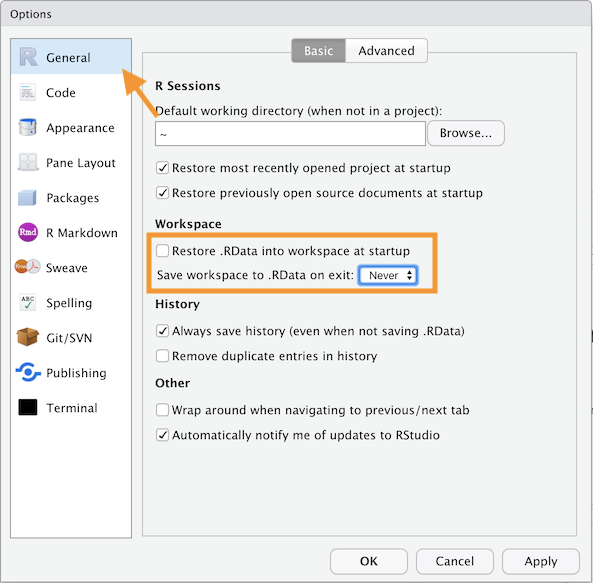
\includegraphics{images/rstudio-startup-and-exit}
    \caption{Réglage de RStudio pour ne pas sauvegarder l'espace
      de travail de R au moment de quitter l'application}
    \label{fig:rstudio:rstudio-startup-and-exit}
  \end{figure}
\item Dans la catégorie \code{Code} et la sous-catégorie
  \code{Editing}, régler l'option \code{Tab width} à \code{4}, tel
  qu'illustré à la \autoref{fig:pratiques:rstudio-tab-width}. Avec ce
  réglage, RStudio indentera par défaut le code de quatre caractères.
  \begin{figure}
    \centering
    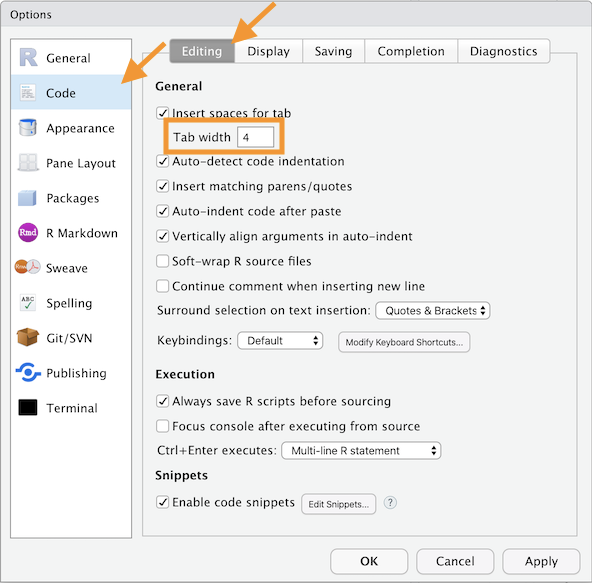
\includegraphics{images/rstudio-tab-width}
    \caption{Réglage de RStudio pour une indentation du code
      de quatre caractères}
    \label{fig:pratiques:rstudio-tab-width}
  \end{figure}
\item Toujours dans la catégorie \code{Code}, mais dans la
  sous-catégorie \code{Saving}, cocher les options \code{Ensure that
    source files end with newline} et \code{Strip trailing horizontal
    whitespace when saving}, puis régler l'option \code{Default text
    encoding} à \code{UTF-8}, tel qu'illustré à la
  \autoref{fig:rstudio:rstudio-utf-8}. RStudio sauvegardera ensuite
  les fichiers de script dans un format portable sur toutes les
  plateformes informatiques et supprimera automatiquement les espaces
  inutiles en fin de ligne.
  \begin{figure}
    \centering
    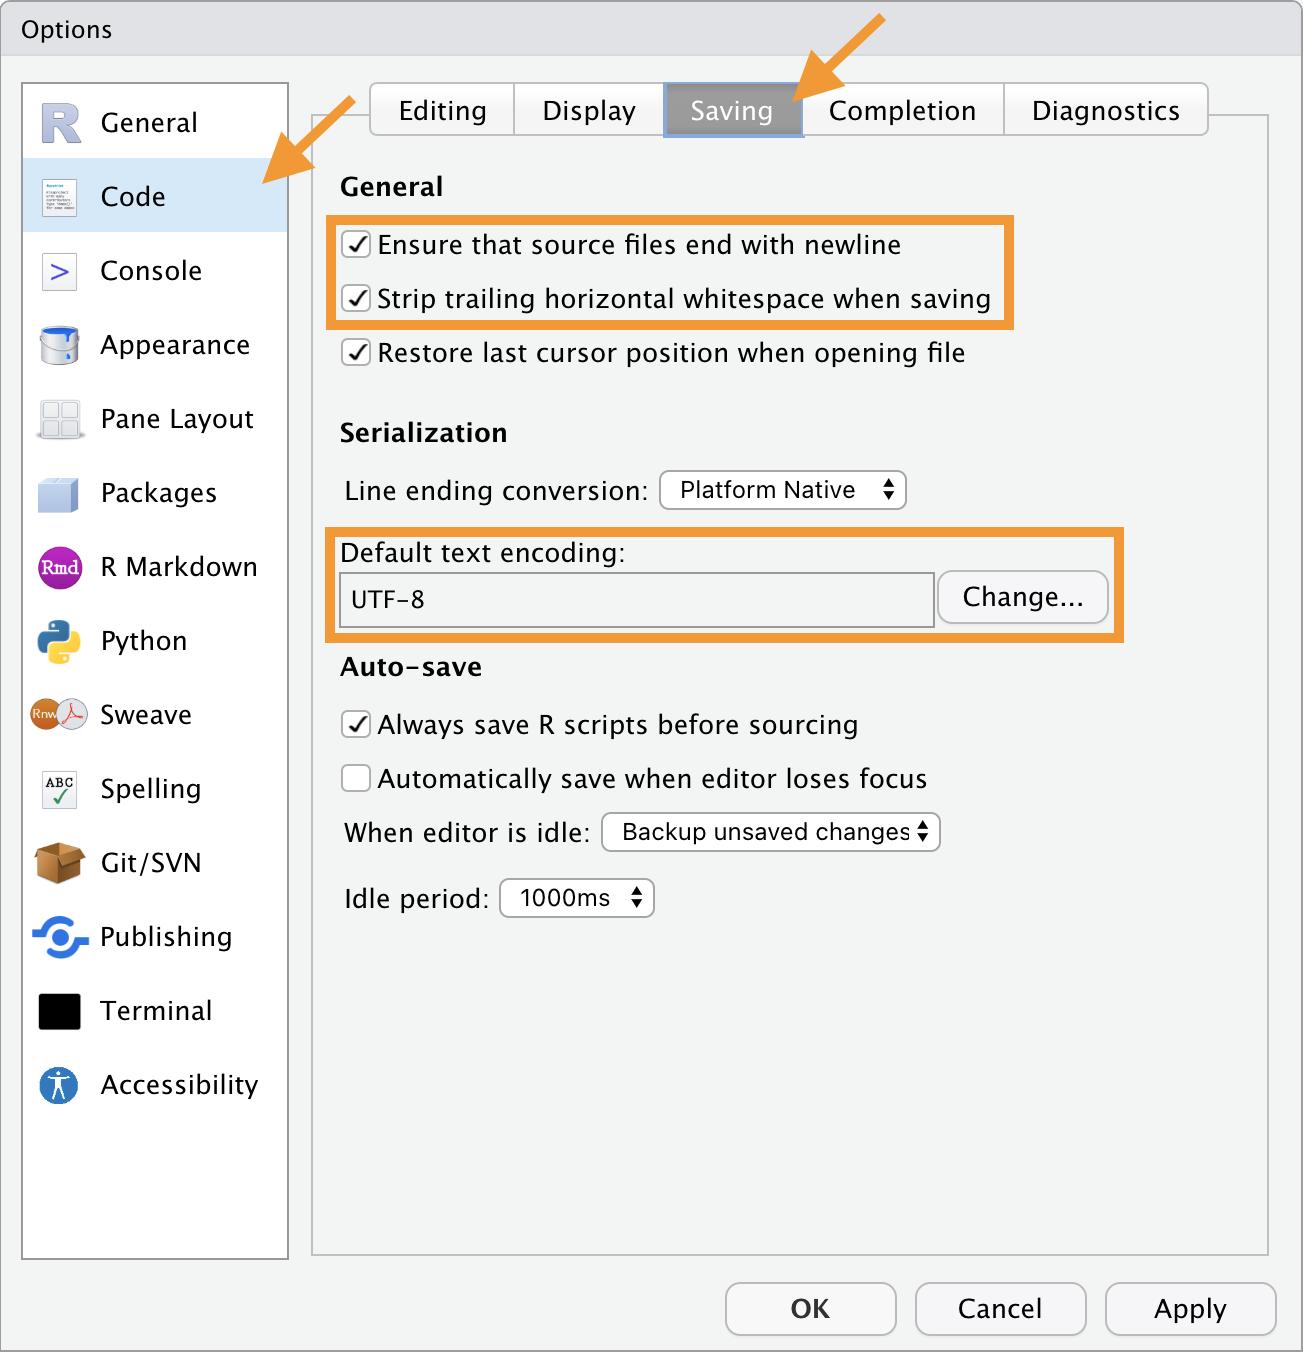
\includegraphics{images/rstudio-utf-8+whitespace}
    \caption{Réglage de RStudio pour la sauvegarde des fichiers dans un
      format portable et sans espaces en fin de ligne}
    \label{fig:rstudio:rstudio-utf-8}
  \end{figure}
\item (Windows seulement) Dans la catégorie \code{Terminal},
  sélectionner \index{Git~Bash}\code{Git~Bash} dans le menu déroulant
  de l'option \code{New Terminals open with}.
\end{enumerate}



\section{Aide et documentation}
\label{sec:rstudio:aide}

La documentation de RStudio se trouve entièrement en ligne. On y
accède par le menu \code{Help}. L'onglet \code{Help} du navigateur de
fichiers (sous-fenêtre en bas à droite) offre également une interface
unifiée pour accéder à l'aide de R et à celle de RStudio.

\index{RStudio|)}

%%% Local Variables:
%%% mode: latex
%%% TeX-engine: xetex
%%% TeX-master: "programmer-avec-r"
%%% coding: utf-8
%%% End:

%%% Copyright (C) 2019 Vincent Goulet
%%%
%%% Ce fichier fait partie du projet
%%% «Programmer avec R»
%%% https://gitlab.com/vigou3/programmer-avec-r
%%%
%%% Cette création est mise à disposition sous licence
%%% Attribution-Partage dans les mêmes conditions 4.0
%%% International de Creative Commons.
%%% https://creativecommons.org/licenses/by-sa/4.0/

\chapter{GNU Emacs et ESS: la base}
\index{Emacs|(}
\label{chap:emacs+ess}

Emacs est l'Éditeur de texte des éditeurs de texte. À l'origine un
éditeur pour les programmeurs (avec des modes spéciaux pour une
multitude de langages différents), Emacs est devenu au fil du temps un
environnement logiciel en soi dans lequel on peut réaliser une foule
de tâches différentes: rédiger des documents {\LaTeX}, interagir avec R,
SAS ou un logiciel de base de données, consulter son courrier
électronique, gérer son calendrier ou même jouer à Tetris!

Cette annexe passe en revue les quelques commandes essentielles pour
commencer à travailler avec GNU Emacs et le mode ESS. L'ouvrage de
\cite{Cameron:Emacs:2004} constitue une excellente référence pour
l'apprentissage plus poussé de l'éditeur.

\setkeys{Gin}{width=370pt} % 1/2 la largeur de l'image insérée
\begin{figure}[t]
  \centering
  \includegraphics{images/emacs.png} \\
  \footnotesize\sffamily\flushleft\vspace{-\baselineskip}%
  Tiré de \href{https://xkcd.com/378/}{XKCD.com}. La commande \code{M-x
    butterfly} existe vraiment dans Emacs\dots\ en référence à cette
  bande dessinée!
\end{figure}
\setkeys{Gin}{width=0.8\textwidth}

\section{Mise en contexte}
\label{sec:emacs+ess:contexte}

Emacs est le logiciel étendard du projet GNU («\emph{GNU is not
  Unix}»), dont le principal commanditaire est la \emph{Free Software
  Foundation} (FSF) à l'origine de tout le mouvement du logiciel
libre. Richard M.\ Stallman, président de la FSF et grand apôtre du
libre, a écrit la première version de Emacs et il continue à ce jour à
contribuer au projet.

Les origines de Emacs remontent au début des années 1980, une époque
où les interfaces graphiques n'existaient pas, le parc informatique
était beaucoup plus hétérogène qu'aujourd'hui (les claviers n'étaient
pas les mêmes d'une marque d'ordinateur à une autre) et les modes de
communication entre les ordinateurs demeuraient rudimentaires.

L'âge vénérable de Emacs transparait à plusieurs endroits, notamment
dans la terminologie inhabituelle, les raccourcis clavier non
conformes aux standards d'aujourd'hui ou la manipulation des fenêtres
qui ne se fait pas avec une souris.

Emacs s'adapte à différentes tâches par l'entremise de \emph{modes}
qui modifient son comportement ou lui ajoutent des fonctionnalités.

L'un de ces modes est ESS \citep[\emph{Emacs Speaks
  Statistics},][]{ESS}. ESS permet d'interagir avec des logiciels
statistiques (en particulier R, S+ et SAS) directement depuis Emacs.
Quelques-uns des développeurs de ESS sont aussi des développeurs de R,
d'où la grande compatibilité entre les deux logiciels. Lorsque ESS est
installé, le mode est activé automatiquement en ouvrant dans Emacs un
fichier dont le nom se termine par l'extension \code{.R}.


\section{Installation}
\label{sec:emacs+ess:installation}

Le présent auteur prépare des distributions modifiées de GNU~Emacs
pour \link{https://vigou3.github.io/emacs-modified-windows/}{Windows}
et pour \link{https://vigou3.github.io/emacs-modified-macos/}{macOS}
qui intègrent le mode ESS.

Sous Linux, GNU Emacs et le mode ESS font normalement partie de toutes
les distributions.

\section{Description sommaire}
\label{sec:emacs+ess:description}

Au lancement, Emacs affiche un écran d'information contenant des liens
vers différentes ressources. Cet écran disparait dès que l'on appuie
sur une touche. La fenêtre Emacs se divise en quatre zones principales
(voir la \autoref{fig:ess:emacswindow}):
\begin{enumerate}
\item tout au haut de la fenêtre (ou de l'écran sous macOS), on trouve
  l'habituelle barre de menu dont le contenu change selon le mode dans
  lequel se trouve Emacs;
\item l'essentiel de la fenêtre sert à afficher un \emph{buffer}, soit
  le contenu d'un fichier ouvert ou l'invite de commande d'un
  programme externe;
\item la ligne de mode est le séparateur horizontal contenant diverses
  informations sur le fichier ouvert et l'état de Emacs;
\item le \emph{minibuffer} est la région au bas de la fenêtre où l'on
  entre des commandes et reçoit de l'information de Emacs.
\end{enumerate}
Il est possible de séparer la fenêtre Emacs en sous-fenêtres pour
afficher plusieurs \emph{buffers} à la fois. Il y a alors une ligne de
mode pour chaque \emph{buffer}.

\begin{figure}[t]
  %% Capture d'écran
  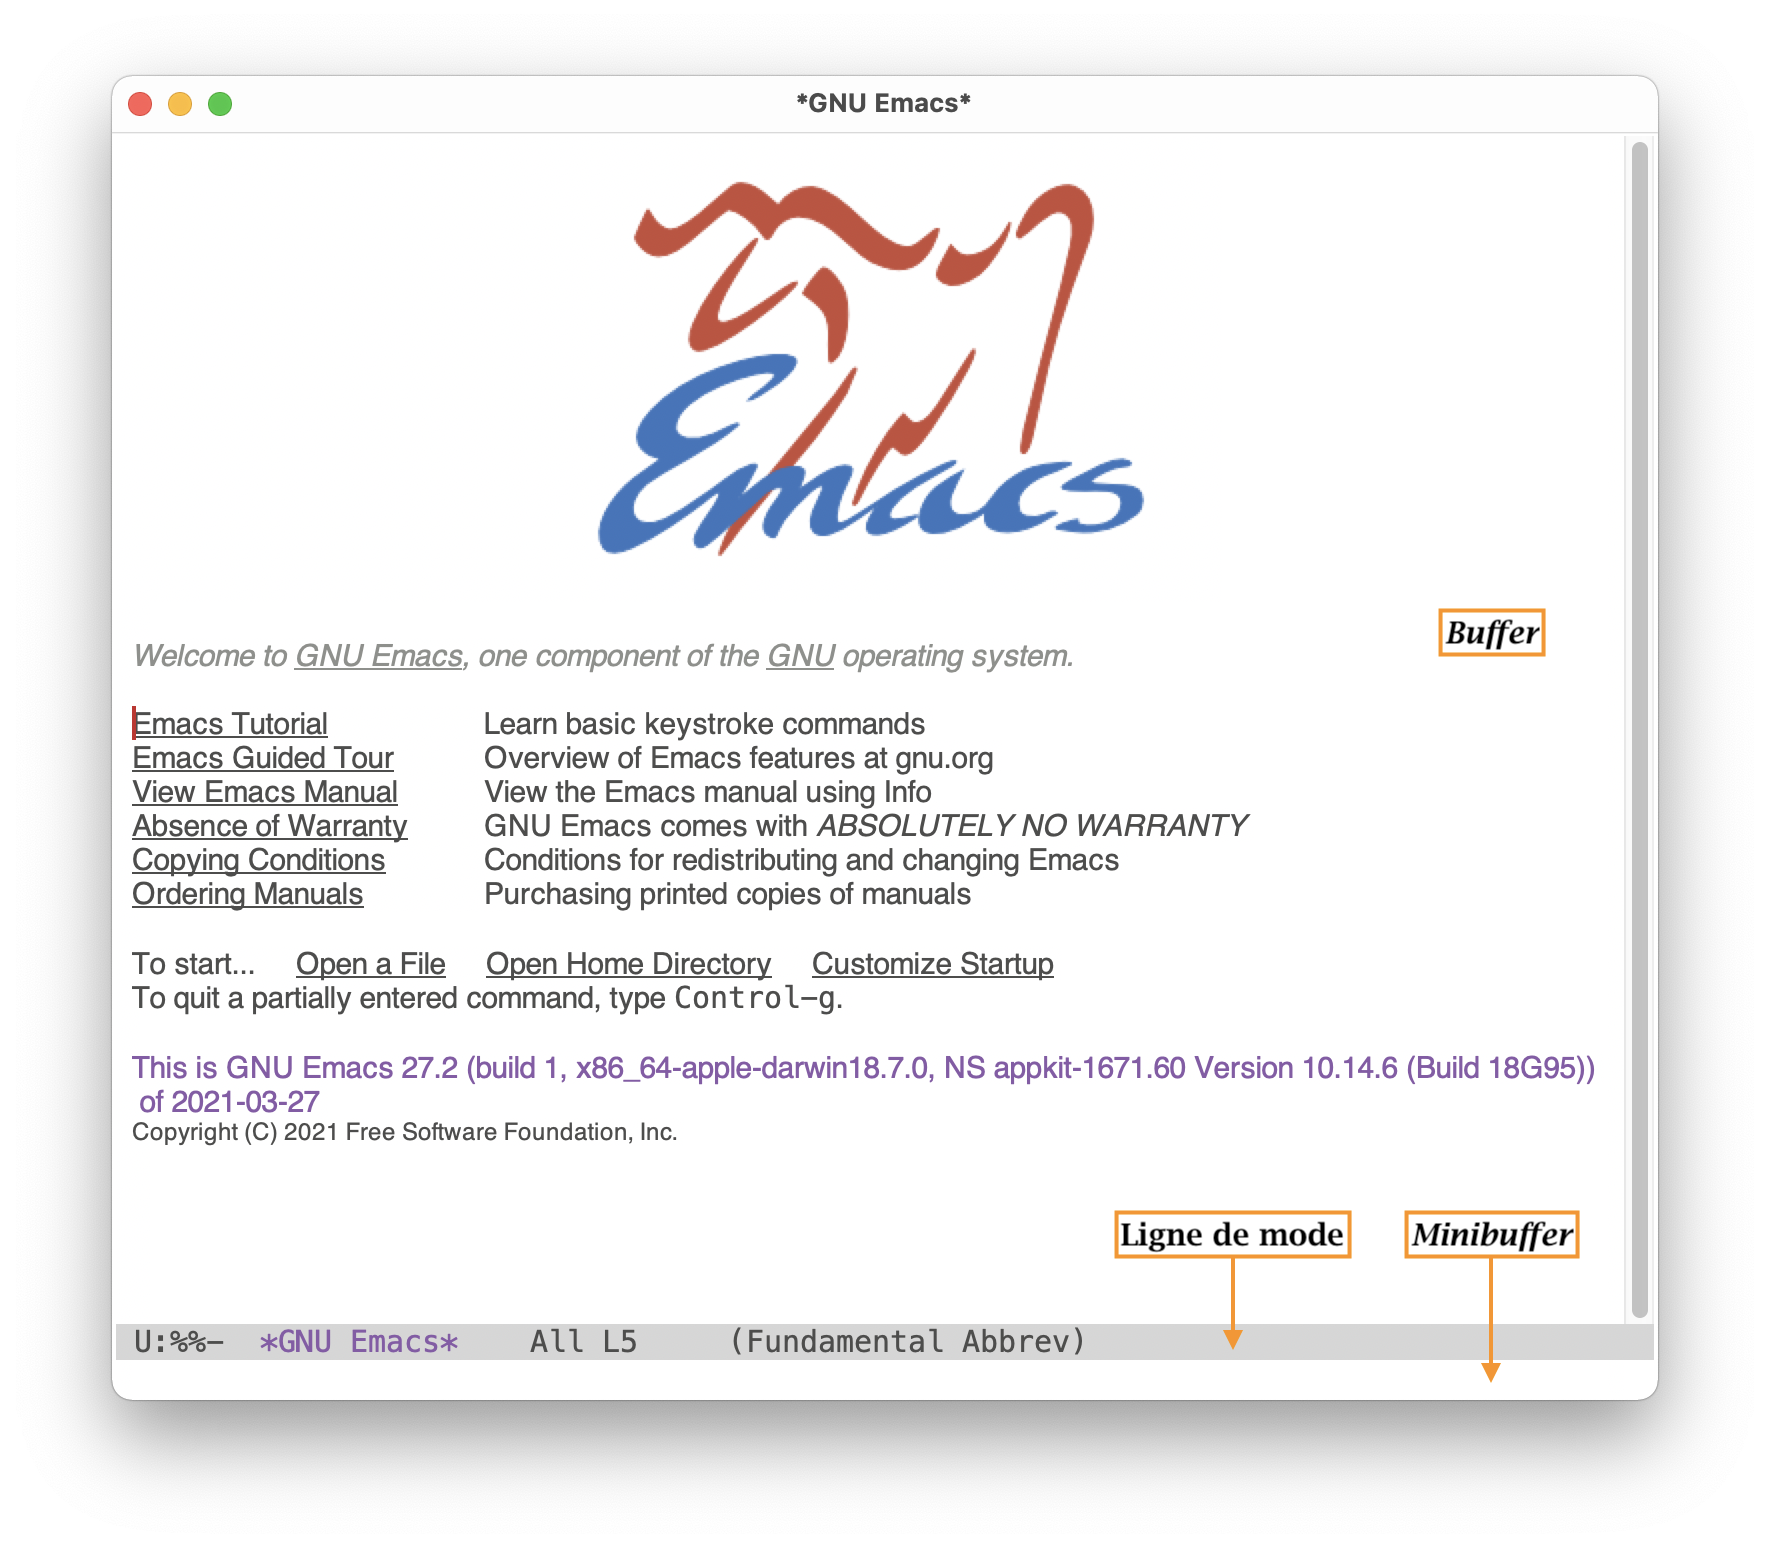
\includegraphics{images/emacswindow-screenshot}

  \begingroup
  \TPoptions{absolute=false}
  %% Identification de la barre de menu
  \begin{textblock}{0.35}(7.38,-6.58)
    \Large\faLongArrowRight
  \end{textblock}
  \begin{textblock}{1.75}(7.88,-6.59)
    \footnotesize\sffamily Barre de menu
  \end{textblock}

  %% Identification du buffer
  \begin{textblock}{0.35}(7.38,-3.38)
    \Large\faLongArrowRight
  \end{textblock}
  \begin{textblock}{1.75}(7.88,-3.39)
    \footnotesize\sffamily \emph{Buffer}
  \end{textblock}

  %% Identification de la mode line
  \begin{textblock}{0.35}(7.38,-0.28)
    \Large\faLongArrowRight
  \end{textblock}
  \begin{textblock}{1.75}(7.88,-0.29)
    \footnotesize\sffamily Ligne de mode
  \end{textblock}

  %% Identification du minibuffer
  \begin{textblock}{0.35}(7.38,-0.08)
    \Large\faLongArrowRight
  \end{textblock}
  \begin{textblock}{1.75}(7.88,-0.09)
    \footnotesize\sffamily \emph{Minibuffer}
  \end{textblock}
  \endgroup
  \caption[Fenêtre de GNU~Emacs sous macOS]{Fenêtre de GNU~Emacs et
    ses différentes parties au lancement de l'application sous macOS.
    Sous Windows et Linux, la barre de menu se trouve à l'intérieur de
    la fenêtre.}
  \label{fig:ess:emacswindow}
\end{figure}


\section{\emph{Emacs-ismes} et \emph{Unix-ismes}}
\label{sec:emacs+ess:ismes}

Emacs possède sa propre terminologie qu'il vaut mieux connaitre
lorsque l'on consulte la documentation. De plus, l'éditeur utilise des
conventions du monde Unix qui sont moins usitées sur les plateformes
Windows et macOS.

\begin{itemize}
\item Dans les définitions de raccourcis claviers:
  \begin{itemize}
  \item \code{C} est la touche \code{Contrôle} (\ctlkey);
  \item \code{M} est la touche \code{Meta}, qui correspond à la touche
    \code{Alt} de gauche sur un PC ou la touche \code{Option}
    (\optkey) sur un Mac (toutefois, voir l'encadré à la
    \autopageref{fig:ess:meta});
  \item \code{ESC} est la touche \code{Échap} (\esckey) et
    est équivalente à \code{Meta};
  \item \code{SPC} est la barre d'espacement;
  \item \code{DEL} est la touche \code{Retour arrière} (\delkey) ---
    \emph{et non la touche} \code{Supprimer}.
  \item \code{RET} est la touche \code{Entrée} (\returnkey);
  \end{itemize}
\item Toutes les fonctionnalités de Emacs correspondent à une commande
  qui peut être tapée dans le \emph{minibuffer}. \code{M-x} démarre
  l'invite de commande.
\item Le caractère \,\verb=~=\, représente le dossier vers lequel
  pointe la variable d'environnement \code{\$HOME} (Linux, macOS) ou
  \code{\%HOME\%} (Windows). C'est le dossier par défaut de Emacs.
\item La barre oblique (\code{/}) est utilisée pour séparer les
  dossiers dans les chemins d'accès aux fichiers, même sous Windows.
\item En général, il est possible d'appuyer sur \code{TAB} dans le
  \emph{minibuffer} pour compléter les noms de fichiers ou de
  commandes.
\end{itemize}

\begin{figure}[t]
  \refstepcounter{dummy}
  \label{fig:ess:meta}
  \begin{titled-frame}{Configuration de la touche Meta sous macOS}
    Par défaut sous macOS, la touche \code{Meta} est assignée à
    \code{Option} (\optkey). Sur les claviers français, cela empêche
    d'accéder à certains caractères spéciaux tels que {\og}[{\fg},
    «]», «\{» ou «\}».

    Une solution à cette fâcheuse situation consiste à assigner
    la touche \code{Meta} à \code{Commande} (\cmdkey). Cela bloque
    alors l'accès à certains raccourcis Mac, mais la situation est
    moins critique ainsi.

    Pour assigner la touche \code{Meta} à \code{Commande} (\cmdkey) et
    laisser la touche \code{Option} (\optkey) jouer son rôle usuel, il
    suffit d'insérer les lignes suivantes dans son fichier de
    configuration \code{.emacs} (voir la
    \autoref{sec:emacs+ess:configuration}):
\begin{verbatim}
(setq-default ns-command-modifier 'meta)
(setq-default ns-option-modifier 'none)
\end{verbatim}
  \end{titled-frame}
\end{figure}



\section{Commandes de base}
\label{sec:emacs+ess:commandes}

Emacs comporte une pléthore de commandes, il serait donc futile de
tenter d'en faire une liste exhaustive ici. Nous nous contenterons de
mentionner les commandes les plus importantes regroupées par tâche.

\subsection{Les essentielles}
\label{sec:emacs+ess:commandes:essentielles}

\begin{ttscript}{M-x}
\item[\code{M-x}] démarrer l'invite de commande
\item[\code{C-g}] bouton de panique: annuler, quitter! Presser plus
  d'une fois au besoin.
\end{ttscript}

\subsection{Manipulation de fichiers}
\label{sec:emacs+ess:commandes:fichiers}

Entre parenthèses, le nom de la commande Emacs correspondante. On peut
entrer cette commande dans le \emph{minibuffer} au lieu d'utiliser le
raccourci clavier.

\tipbox{Il n'existe pas de commande «nouveau
  fichier» dans Emacs. Pour créer un nouveau fichier, il suffit
  d'ouvrir un fichier qui n'existe pas déjà.\index{Emacs!nouveau fichier}}

\begin{ttscript}{C-x C-w}
\item[\code{C-x C-f}] ouvrir un fichier (\code{find-file})
\item[\code{C-x C-s}] sauvegarder
  (\code{save-buffer})\index{Emacs!sauvegarder}
\item[\code{C-x C-w}] sauvegarder sous
  (\code{write-file})\index{Emacs!sauvegarder sous}
\item[\code{C-x k}] fermer un fichier (\code{kill-buffer})
  \\[\baselineskip]
\item[\code{C-\_}] annuler (pratiquement illimité); aussi
  \code{C-x u} (\code{undo})
  \\
\item[\code{C-s}] recherche incrémentale avant
  (\code{isearch-forward})
\item[\code{C-r}] Recherche incrémentale arrière
  (\code{isearch-backward})
\item[\code{M-\%}] rechercher et remplacer
  (\code{query-replace})\index{Emacs!rechercher et remplacer}
\end{ttscript}


\subsection{Déplacements simples du curseur}
\index{Emacs!déplacement du curseur}
\label{sec:emacs+ess:commandes:deplacement}

\begin{ttscript}{C-DEL | C-w}
\item[\code{C-b} | \code{C-f}] déplacer d'un caractère vers
  l'arrière~|~l'avant \newline
  (\code{backward-char} | \code{forward-char})
\item[\code{C-a} | \code{C-e}] aller au début~|~fin de la ligne \newline
  (\code{move-beginning-of-line} | \code{move-end-of-line})
\item[\code{C-p} | \code{C-n}] aller à la ligne précédente~|~suivante \newline
  (\code{previous-line} | \code{next-line})
\item[\code{M-<} | \code{M->}] aller au début~|~fin du fichier \newline
  (\code{beginning-of-buffer} | \code{end-of-buffer})
  \\
\item[\code{DEL} | \code{C-d}] effacer le caractère à
  gauche~|~droite du curseur  \newline
  (\code{delete-backward-char} | \code{delete-char})
\item[\code{M-DEL} | \code{M-d}] effacer le mot à gauche~|~droite
  du curseur  \newline
  (\code{backward-kill-word} | \code{kill-word})
\item[\code{C-k}] supprimer jusqu'à la fin de la ligne (\code{kill-line})
\end{ttscript}

\osxbox{Plusieurs des raccourcis clavier de Emacs composés avec la
  touche \code{Contrôle} (\ctlkey) sont valides sous macOS. Par
  exemple, \ctlkey\,\code{A} et \ctlkey\,\code{E} déplacent le curseur
  au début et à la fin de la ligne dans les champs texte.}


\subsection{Sélection de texte, copier, coller, couper}
\index{Emacs!sélection}
\label{sec:emacs+ess:commandes:selection}

\begin{ttscript}{C-x C-w}
\item[\code{C-SPC}] débute la sélection (\code{set-mark-command})
\item[\code{C-w}] couper la sélection (\code{kill-region})
\item[\code{M-w}] copier la sélection (\code{kill-ring-save})
\item[\code{C-y}] coller (\code{yank})
\item[\code{M-y}] remplacer le dernier texte collé par la
  sélection précédente \newline
  (\code{yank-pop})
\end{ttscript}

\tipbox{Il est possible d'utiliser les raccourcis clavier usuels de
  Windows (\code{C-c}, \code{C-x}, \code{C-v}) et macOS
  (\cmdkey\,\code{C}, \cmdkey\,\code{X}, \cmdkey\,\code{V}) en
  activant le mode CUA dans le menu \code{Options}.}

\windowsbox{ On peut copier-coller directement avec la souris dans Windows en
  sélectionnant du texte puis en appuyant sur le bouton central (ou la
  molette) à l'endroit souhaité pour y copier le texte.}


\subsection{Manipulation de fenêtres}
\label{sec:emacs+ess:commandes:fenetres}

\begin{ttscript}{C-x C-w}
\item[\code{C-x b}] changer de \emph{buffer}
  (\code{switch-buffer})
\item[\code{C-x 2}] séparer l'écran en deux fenêtres
  (\code{split-window-vertically})
\item[\code{C-x 1}] conserver uniquement la fenêtre courante \newline
  (\code{delete-other-windows})
\item[\code{C-x 0}] fermer la fenêtre courante
  (\code{delete-window})
\item[\code{C-x o}] aller vers une autre fenêtre lorsqu'il y en a
  plus d'une \newline
  (\code{other-window})
\end{ttscript}

\subsection{Manipulation de fichiers de script dans le mode ESS}
\index{Emacs!mode ESS|(}
\label{sec:emacs+ess:commandes:script}

Le mode ESS dispose de fonctions «intelligentes» qui facilitent
grandement la manipulation des fichiers de script. Les deux
principales commandes à connaitre sont les suivantes:
\begin{ttscript}{C-x C-w}
\item[\code{C-RET}] évaluer dans le processus R la ligne sous le
  curseur ou la région sélectionnée, puis déplacer le curseur à la
  prochaine expression \newline
  (\code{ess-eval-region-or-line-and-step})
\item[\code{C-c C-c}] évaluer dans le processus R la région
  sélectionnée, la fonction ou le paragraphe (tout bloc entre deux
  lignes blanches) dans lequel se trouve le curseur, puis déplacer le
  curseur à la prochaine expression \newline
  (\code{ess-eval-region-or-function-or-paragraph-and-step})
\end{ttscript}
Les quelques autres fonctions utiles sont:
\begin{ttscript}{C-x C-w}
\item[\code{\_}] insérer le symbole d'affectation \verb*| <- | (sauf
  dans les champs texte et dans les commentaires);
  appuyer deux fois consécutives pour obtenir le caractère de
  soulignement \newline
  (\code{ess-smart-S-assign})
\item[\code{C-c C-z}] déplacer le curseur vers le processus R \newline
  (\code{ess-switch-to-inferior-or-script-buffer})
\item[\code{C-c C-f}] évaluer le code de la fonction courante dans
  le processus R \newline
  (\code{ess-eval-function})
\item[\code{C-c C-l}] évaluer le code du fichier courant en entier dans
  le processus R \newline
  (\code{ess-load-file})
\item[\code{C-c C-v}] aide sur une commande R
  (\code{ess-display-help-on-object})
\end{ttscript}

\subsection{Interaction avec l'invite de commande R}
\label{sec:emacs+ess:commandes:invite}

\begin{ttscript}{M-p |M-n}
\item[\code{M-p} | \code{M-n}] commande précédente~|~suivante
  dans l'historique \newline
  (\code{previous-matching-history-from-input} | \newline
  \code{next-matching-history-from-input})
\item[\code{C-c C-z}] déplacer le curseur vers le fichier de script
  courant \newline
  (\code{ess-switch-to-inferior-or-script-buffer})
\item[\code{M-h}] sélectionner le résultat de la dernière commande \newline
  (\code{mark-paragraph})
\item[\code{C-c C-o}] effacer le résultat de la dernière commande \newline
  (\code{comint-delete-output})
\item[\code{C-c C-v}] aide sur une commande R
  (\code{ess-display-help-on-object})
\item[\code{C-c C-q}] terminer le processus R (\code{ess-quit})
\end{ttscript}

\subsection{Consultation des rubriques d'aide de R}
\label{sec:emacs+ess:commandes:aide}

\begin{ttscript}{m, m}
\item[\code{p} | \code{n}] aller à la section précédente~|~suivante de
  la rubrique \newline
  (\code{ess-skip-to-previous-section} |
  \code{ess-skip-to-next-section})
\item[\code{s a}] aller à la section de la liste des arguments \emph{(Arguments)}
\item[\code{s D}] aller à la section des détails sur la fonction \emph{(Details)}
\item[\code{s v}] aller à la section sur la valeur retournée par la
  fonction \emph{(Value)}
\item[\code{s s}] aller à la section des fonctions apparentée \emph{(See Also)}
\item[\code{s e}] aller à la section des exemples \emph{(Examples)}
\item[\code{l}] évaluer la ligne sous le curseur; pratique pour
  exécuter les exemples \newline
  (\code{ess-eval-line-and-step})
\item[\code{r}] évaluer la région sélectionnée (\code{ess-eval-region})
\item[\code{h}] ouvrir une nouvelle rubrique d'aide, par défaut pour
  le mot se trouvant sous le curseur
  (\code{ess-display-help-on-object})
\item[\code{q}] retourner au processus ESS en laissant la rubrique
  d'aide visible \newline
  (\code{ess-switch-to-end-of-ESS})
\item[\code{x}] fermer la rubrique d'aide et retourner au processus
  ESS \newline
  (\code{ess-kill-buffer-and-go})
\end{ttscript}



\section{Anatomie d'une session de travail (ter)}
\label{sec:emacs+ess:session}

On reprend ici la description de la type présentée à la
\autoref{sec:presentation:session}, mais en expliquant comment
compléter chaque étape dans Emacs avec le mode ESS. Sont intercalés
dans les instructions les raccourcis clavier des commandes Emacs et
les accès par les menus, le cas échéant.

\begin{enumerate}
\item Lancer Emacs et ouvrir un fichier de script.
  \begin{trivlist}
  \item
    \makebox[0.28\linewidth][l]{%
      \colorbox{codebg}{\code{C-x C-f}}}
    \hfill
    \makebox[0.68\linewidth][l]{%
      \colorbox{codebg}{\code{File|Open File...}}}
  \end{trivlist}
  En spécifiant un nom de fichier qui n'existe pas déjà, on crée un
  nouveau fichier de script. S'assurer de terminer le nom du nouveau
  fichier par \code{.R} pour que Emacs reconnaisse automatiquement
  qu'il s'agit d'un fichier de script R.
\item Démarrer un processus R à l'intérieur de Emacs.
  \begin{trivlist}
  \item
    \makebox[0.28\linewidth][l]{%
      \colorbox{codebg}{\code{M-x R }\returnkey}}
  \end{trivlist}
  Emacs demandera de spécifier de répertoire de travail
  (\emph{starting data directory}). Accepter la valeur par défaut ou
  indiquer un autre dossier.
  \begin{trivlist}
  \item
    \makebox[0.28\linewidth][l]{%
      \colorbox{codebg}{\code{\textasciitilde/ = }\returnkey}}
  \end{trivlist}
  Un éventuel message de Emacs à l'effet que le fichier
  \code{.Rhistory} n'a pas été trouvé est sans conséquence et peut
  être ignoré.
\item Composer le code. Lors de cette étape, on se déplacera souvent
  du fichier de script à la ligne de commande afin d'essayer diverses
  expressions. On exécutera également des parties seulement du code se
  trouvant dans le fichier de script. Les commandes les plus utilisées
  sont alors:
  \begin{trivlist}
  \item
    \makebox[0.28\linewidth][l]{%
      \colorbox{codebg}{\code{C+RET}}}
    \hfill
    \makebox[0.68\linewidth][l]{%
      \colorbox{codebg}{\code{ESS|Eval region | line}}}
  \item
    \makebox[0.28\linewidth][l]{%
      \colorbox{codebg}{\code{C-c C-c}}}
    \hfill
    \makebox[0.68\linewidth][l]{%
      \colorbox{codebg}{\code{ESS|Eval region | func | para \& step}}}
  \item
    \makebox[0.28\linewidth][l]{%
      \colorbox{codebg}{\code{C-c C-z}}}
    \hfill
    \makebox[0.68\linewidth][l]{%
      \colorbox{codebg}{\code{ESS|Process|Switch to process buffer}}}
  \end{trivlist}
\item Sauvegarder le fichier de script.
  \begin{trivlist}
  \item
    \makebox[0.28\linewidth][l]{%
      \colorbox{codebg}{\code{C-x C-s}}}
    \hfill
    \makebox[0.68\linewidth][l]{%
      \colorbox{codebg}{\code{File|Save}}}
  \end{trivlist}
  Les quatrième et cinquième caractères de la ligne de mode changent
  de \,\verb|**|\, à \,\verb|--|.
\item Sauvegarder si désiré l'espace de travail de R avec
  \code{save.image()}\index{save.image@\code{save.image}}. Cela n'est
  habituellement pas nécessaire à moins que l'espace de travail ne
  contienne des objets importants ou longs à recréer.
\item Quitter le processus R.
  \begin{trivlist}
  \item
    \makebox[0.28\linewidth][l]{%
      \colorbox{codebg}{\code{C-c C-q}}}
    \hfill
    \makebox[0.68\linewidth][l]{%
      \colorbox{codebg}{\code{iESS|Quit}}}
  \end{trivlist}
  Cette commande de ESS se charge de fermer tous les fichiers associés
  au processus R. On peut ensuite quitter Emacs en fermant
  l'application de la manière usuelle.
\end{enumerate}
\index{Emacs!mode ESS|)}

\videobox{\link{https://youtu.be/KtmFDm2AKM4}{Anatomie d'une session de travail
    avec GNU Emacs}}{%
  La session de travail type avec GNU Emacs ci-dessus fait aussi l'objet
  d'\link{https://youtu.be/KtmFDm2AKM4}{une vidéo}.}


\section{Configuration de l'éditeur}
\label{sec:emacs+ess:configuration}

Une des grandes forces de Emacs est qu'à peu près chacune de ses
facettes est configurable: couleurs, polices de caractère, raccourcis
clavier, etc.

La configuration de Emacs repose sur des commandes réunies dans un
nommé \code{.emacs} (le point est important!) que Emacs lit au
démarrage. Le fichier \code{.emacs} doit se trouver dans le dossier
\,\verb=~/=, c'est-à-dire dans le dossier de départ de l'utilisateur
sous Linux et macOS, et dans le dossier référencé par la variable
d'environnement \code{\%HOME\%} sous Windows.

\videobox{\link{https://youtu.be/jdtjBBkfhO0}{Création de fichiers de
    configuration pour Emacs et R}}{%
  Visionnez la vidéo portant sur la
  \link{https://youtu.be/jdtjBBkfhO0}{création de fichiers de
    configuration} pour Emacs et R.}


\section{Aide et documentation}
\label{sec:emacs+ess:aide}

Emacs possède son propre système d'aide très exhaustif, mais dont la
navigation est peu intuitive selon les standards d'aujourd'hui.
Consulter le menu \code{Help}.

Autrement, on trouvera dans les sites respectifs des deux projets les
manuels de \link{https://www.gnu.org/software/emacs}{Emacs} et de
\link{https://ess.r-project.org}{ESS}.

Enfin, si le désespoir vous prend au cours d'une séance de codage
intensive, vous pouvez toujours consulter le psychothérapeute Emacs.
On le trouve, bien entendu, dans le menu \code{Help}!

\index{Emacs|)}

%%% Local Variables:
%%% mode: latex
%%% TeX-engine: xetex
%%% TeX-master: "programmer-avec-r"
%%% coding: utf-8
%%% End:

%%% Copyright (C) 2017-2022 Vincent Goulet
%%%
%%% Ce fichier fait partie du projet
%%% «Programmer avec R»
%%% https://gitlab.com/vigou3/programmer-avec-r
%%%
%%% Cette création est mise à disposition sous licence
%%% Attribution-Partage dans les mêmes conditions 4.0
%%% International de Creative Commons.
%%% https://creativecommons.org/licenses/by-sa/4.0/

\chapter{Solutions des exercices}
\label{chap:solutions}

%% Ce fichier ne sert qu'à disposer les solutions des exercices à la
%% fin du document. Le texte des solutions se trouve avec leur
%% exercice correspondant, dans les fichiers des chapitres.

\input{solutions-informatique}
\input{solutions-algorithmes}
\input{solutions-bases}
\input{solutions-donnees}
\input{solutions-pratiques}
\input{solutions-tri}
\input{solutions-debogage}
\input{solutions-import-export}
\input{solutions-texte}
\input{solutions-environnement}

%%% Local Variables:
%%% mode: latex
%%% TeX-engine: xetex
%%% TeX-master: "programmer-avec-r"
%%% coding: utf-8
%%% End:


\bibliography{r,stat,informatique,vg}

\cleardoublepage
\chaptermark{Index}
\printindex

\cleartoverso
\pagestyle{empty}
%%% Copyright (C) 2014-2024 Vincent Goulet
%%%
%%% Ce fichier fait partie du projet
%%% «Programmer avec R»
%%% https://gitlab.com/vigou3/programmer-avec-r
%%%
%%% Cette création est mise à disposition sous licence
%%% Attribution-Partage dans les mêmes conditions 4.0
%%% International de Creative Commons.
%%% https://creativecommons.org/licenses/by-sa/4.0/

\vspace*{\fill}

\begingroup
\calccentering{\unitlength}
\begin{adjustwidth*}{\unitlength}{-\unitlength}
  \begin{flushleft}
    \small %
    Ce document a été produit avec le système de mise en page
    {\XeLaTeX}. Le texte principal est composé en Lucida Bright~OT
    11~points, les mathématiques en Lucida Bright Math~OT, le code
    informatique en Lucida Grande Mono~DK et les titres en Fira~Sans.
    Des icônes proviennent de la police Font~Awesome. Les graphiques
    ont été réalisés avec R.
  \end{flushleft}
\end{adjustwidth*}
\endgroup
\vfill


\cleartoverso
%%% Copyright (C) 2021 Vincent Goulet
%%%
%%% Ce fichier fait partie du projet
%%% «Programmer avec R»
%%% https://gitlab.com/vigou3/programmer-avec-r
%%%
%%% Cette création est mise à disposition sous licence
%%% Attribution-Partage dans les mêmes conditions 4.0
%%% International de Creative Commons.
%%% https://creativecommons.org/licenses/by-sa/4.0/

\begingroup
\TPGrid{8}{64}
\textblockorigin{0mm}{0mm}
\setlength{\parindent}{0mm}
\setlength{\bandeorwidth}{12.8125\TPVertModule} % == 4\logoheight
\setlength{\banderougewidth}{\paperwidth}
\addtolength{\banderougewidth}{-\bandeorwidth}
\setlength{\bandeorheight}{\TPVertModule}
\setlength{\banderougeheight}{\TPVertModule}

%% bandeau identitaire arrière
\begin{textblock*}{\paperwidth}[0,1](0mm,56\TPVertModule)
  \textcolor{or}{\rule{\bandeorwidth}{\TPVertModule}}%      % bande or
  \textcolor{rouge}{\rule{\banderougewidth}{\TPVertModule}} % bande rouge
\end{textblock*}
\endgroup

%%% Local Variables:
%%% mode: latex
%%% TeX-master: "programmer-avec-r"
%%% TeX-engine: xetex
%%% End:


\end{document}

%%% Local Variables:
%%% mode: latex
%%% TeX-engine: xetex
%%% TeX-master: t
%%% coding: utf-8
%%% End:
